%%%%%%%% ICML 2021 EXAMPLE LATEX SUBMISSION FILE %%%%%%%%%%%%%%%%%

\documentclass{article}

% Recommended, but optional, packages for figures and better typesetting:
\usepackage{microtype}
\usepackage{graphicx}
\usepackage{subfigure}
\usepackage{booktabs} % for professional tables

% hyperref makes hyperlinks in the resulting PDF.
% If your build breaks (sometimes temporarily if a hyperlink spans a page)
% please comment out the following usepackage line and replace
% \usepackage{icml2021} with \usepackage[nohyperref]{icml2021} above.


% Attempt to make hyperref and algorithmic work together better:
\newcommand{\theHalgorithm}{\arabic{algorithm}}

% Use the following line for the initial blind version submitted for review:
\usepackage{icml2021}
%!TEX root =  autocontgrlp.tex

\usepackage{multicol}
\usepackage{multirow}
\usepackage{dsfont}

%\setlength{\marginparwidth}{13mm}
\usepackage[textsize=tiny]{todonotes}
%\usepackage[disable]{todonotes}
\newcommand{\todoch}[2][]{\todo[color=blue!20!white,#1]{C: #2}}
%\usepackage{enumitem}
%\usepackage[fleqn]{amsmath}
\usepackage{amsmath}
\usepackage{hyperref}
\usepackage{cleveref}
\usepackage{mathtools}
\usepackage{graphicx}
\usepackage{times}
\usepackage{helvet}
\usepackage{courier}
\usepackage{paralist}
\usepackage{latexsym}
\usepackage{url}
\usepackage[all]{xy}
\usepackage{amsmath}
\usepackage{amssymb}
\usepackage{amsthm}
\usepackage{nccmath} % mfrac
\usepackage{comment}
%\usepackage{enumitem}
\usepackage{paralist}
\usepackage{xcolor}
%\usepackage[colorlinks=true,linkcolor=blue,citecolor=purple]{hyperref}
%\usepackage{hyperref}
\usepackage{graphicx}
\usepackage{pifont}
%\usepackage{algorithm}
%\usepackage{algorithmic}
%\usepackage{pseudocode}
%\usepackage{algpseudocode}
\usepackage{savesym}
\savesymbol{AND}
\usepackage{xspace}
\usepackage{tikz}
\usepackage{pgfplots}
\usepackage{pgf}
%\usepackage{algorithm}
%\usepackage{algorithmic}
\usepackage{xspace}
\usepackage{comment}
\usepackage{placeins}
%\usepackage[capitalize]{cleveref}
%\usepackage{caption}

%\usepackage{style/ssltr}
%\usepackage{style/macros}
\if0
\usetikzlibrary{intersections}
\usetikzlibrary{arrows,calc,fit,patterns,plotmarks,shapes.geometric,shapes.misc,shapes.symbols,   shapes.arrows,   shapes.callouts,   shapes.multipart,   shapes.gates.logic.US,   shapes.gates.logic.IEC,   er,   automata,   backgrounds,   chains,   topaths,   trees,   petri,   mindmap,   matrix,   calendar,   folding, fadings,   through,   positioning,   scopes,   decorations.fractals,   decorations.shapes,   decorations.text,   decorations.pathmorphing,   decorations.pathreplacing,   decorations.footprints,   decorations.markings, shadows,circuits}
\tikzstyle{decision}=[diamond,draw]
\tikzstyle{line}=[draw]
\tikzstyle{elli}=[draw,ellipse]
\tikzstyle{arrow} = [thick]
\fi
%\usepackage{subfig}

\newcommand{\rsa}{\rightsquigarrow}

\newcommand{\mb}{\mbox{ }}
\newcommand{\one}{\mathbf{1}}
\newcommand{\zero}{\mathbf{0}}
\newcommand{\nn}{\nonumber}


\newcommand{\R}{\Re} %{\mathbb{R}}
\newcommand{\Rm}{\mathbf{R}_{\min}}
\newcommand{\ra}{\rightarrow}
\newcommand{\om}{\otimes}
\newcommand{\op}{\oplus}
\newcommand{\RA}{\Rightarrow}
\newcommand{\LA}{\Leftarrow}
%\newcommand{\E}{\mathbb{E}}
\newcommand{\E}[1]{\mathbb{E}\left[#1\right]}
\newcommand{\lmin}[1]{\lambda_{\min}\left(#1\right)}
\newcommand{\T}{\mathcal{T}}
\newcommand{\B}{\mathcal{B}}
\newcommand{\F}{\mathcal{F}}
\newcommand{\C}{\mathcal{C}}
\newcommand{\M}{\mathcal{M}}
\newcommand{\N}{\mathcal{N}}

\newcommand{\I}{\mathcal{I}}

\newcommand{\mm}{m_{-}}
\newcommand{\mdm}{m'_{-}}
\newcommand{\Tvm}{\Theta^{v,\mm}}
\newcommand{\Tvmd}{\Theta^{v,\mdm}}


%\newcommand{\Tb}{\mathbf{\Theta}}
%\newcommand{\Tv}{\mathbf{\Theta}^v}
%\newcommand{\Tw}{\mathbf{\Theta}^w}
\newcommand{\tv}{\theta^v}

\newcommand{\Tb}{{\Theta}}
\newcommand{\Tv}{{\Theta}^v}
\newcommand{\Tw}{{\Theta}^w}
\newcommand{\Tg}{{\Theta}^g}

\newcommand{\tg}{\theta^g}
%\newcommand{\Tg}{\mathbf{\Theta}^g}
\newcommand{\Tt}{\Theta}

\newcommand{\G}{\mathcal{G}}

\DeclareMathOperator{\argmin}{argmin}
\DeclareMathOperator{\argmax}{argmax}
\newcommand{\norm}[1]{\|#1\|}
\newcommand{\inorm}[1]{\|#1\|_{\infty}}
\newcommand{\snorm}[1]{\left\|#1\right\|}
\newcommand{\sinorm}[1]{\left\|#1\right\|_{\infty}}


%\newcommand{\eqdef}{\stackrel{\text{\footnotesize def}}{=}}
%\newcommand{\eqdef}{\stackrel{\Delta}{=}}
\newcommand{\eqdef}{\doteq}
\newcommand{\defeq}{\doteq}

\newcommand{\eps}{\varepsilon}
\renewcommand{\epsilon}{\varepsilon}

\newcommand{\nt}{\nabla_{\Theta}}
\newcommand{\al}{\mathcal{AL}}
\newcommand{\aw}{\mathcal{AW}}
\newcommand{\ap}{\mathcal{AP}}

\newcommand{\keywords}[1]{{\bf Keywords: } #1\par}
%\newenvironment{proof}{{\bf Proof:} }{}
\newtheorem{theorem}{Theorem}[section]
\newtheorem{lemma}[theorem]{Lemma}
\newtheorem{claim}[theorem]{Claim}
\newtheorem{proposition}[theorem]{Proposition}
\newtheorem{corollary}[theorem]{Corollary}
\newtheorem{assumption}{Assumption}
\newtheorem{definition}{Definition}[section]
\newtheorem{remark}{Remark}[section]
\newtheorem{identity}{Identity}[section]
\newtheorem{example}{Example}[section]
\newtheorem{note}{Note}[section]
\newtheorem{notation}{Notation}[section]
\newcommand{\alert}[1]{\textcolor{red}{#1}} 
\newcommand{\J}{\mathcal{J}}
\newcommand{\ip}[1]{\langle #1\rangle}

\def\v{\mathbf{v}}
\def\r{\mathbf{r}}
\def\p{\mathbf{p}}
\def\q{\mathbf{q}}
%\def\R{\mathrm{R}}
\def\Re{\mathbb{R}}
\def\Z{\mathbb{Z}}
\def\P{\mathcal{P}}
\def\S{\mathcal{S}}
\def\A{\mathcal{A}}
\def\X{\mathcal{X}}
\def\U{\mathcal{U}}

%\newcommand{\B}{\mathcal{B}}


\newcommand{\ith}[2][th]{$#2^{\text{#1}}$}
\newcommand{\us}[2]{\underset{#2}{#1}~}
\newcounter{subequation}[equation]
\newcommand{\thesubequationonly}{\alph{subequation}}
\renewcommand{\thesubequation}{\text{\theequation(\thesubequationonly)}}
\newcommand{\subequationitem}{\refstepcounter{subequation}(\thesubequationonly)\thinspace}

\def\mathdisplay#1{%
  \ifmmode \@badmath
  \else
    $\def\@currenvir{#1}%
    \let\dspbrk@context\z@
    \let\tag\tag@in@display \SK@equationtrue %\let\label\label@in@display
    \global\let\df@label\@empty \global\let\df@tag\@empty
    \global\tag@false
    \let\mathdisplay@push\mathdisplay@@push
    \let\mathdisplay@pop\mathdisplay@@pop
    \if@fleqn
      \edef\restore@hfuzz{\hfuzz\the\hfuzz\relax}%
      \hfuzz\maxdimen
      \setbox\z@\hbox to\displaywidth\bgroup
        \let\split@warning\relax \restore@hfuzz
        \everymath\@emptytoks \m@th $\displaystyle
    \fi
%   \fi
}


% If accepted, instead use the following line for the camera-ready submission:
%\usepackage[accepted]{icml2021}```

% The \icmltitle you define below is probably too long as a header.
% Therefore, a short form for the running title is supplied here:
\icmltitlerunning{Submission and Formatting Instructions for ICML 2021}

\begin{document}

\twocolumn[
\icmltitle{Duality Simplifies Neural Tangent Kernel: From Alchemy To Atoms}

% It is OKAY to include author information, even for blind
% submissions: the style file will automatically remove it for you
% unless you've provided the [accepted] option to the icml2021
% package.

% List of affiliations: The first argument should be a (short)
% identifier you will use later to specify author affiliations
% Academic affiliations should list Department, University, City, Region, Country
% Industry affiliations should list Company, City, Region, Country

% You can specify symbols, otherwise they are numbered in order.
% Ideally, you should not use this facility. Affiliations will be numbered
% in order of appearance and this is the preferred way.
\icmlsetsymbol{equal}{*}

\begin{icmlauthorlist}
\icmlauthor{Chandrashekar}{}
\end{icmlauthorlist}

\icmlaffiliation{to}{Department of Computation, University of Torontoland, Torontoland, Canada}
\icmlaffiliation{goo}{Googol ShallowMind, New London, Michigan, USA}
\icmlaffiliation{ed}{School of Computation, University of Edenborrow, Edenborrow, United Kingdom}

\icmlcorrespondingauthor{Cieua Vvvvv}{c.vvvvv@googol.com}
\icmlcorrespondingauthor{Eee Pppp}{ep@eden.co.uk}

% You may provide any keywords that you
% find helpful for describing your paper; these are used to populate
% the "keywords" metadata in the PDF but will not be shown in the document
\icmlkeywords{Machine Learning, ICML}

\vskip 0.3in
]

% this must go after the closing bracket ] following \twocolumn[ ...

% This command actually creates the footnote in the first column
% listing the affiliations and the copyright notice.
% The command takes one argument, which is text to display at the start of the footnote.
% The \icmlEqualContribution command is standard text for equal contribution.
% Remove it (just {}) if you do not need this facility.

%\printAffiliationsAndNotice{}  % leave blank if no need to mention equal contribution
\printAffiliationsAndNotice{\icmlEqualContribution} % otherwise use the standard text.

\begin{abstract}
We consider deep neural networks (DNNs) with \emph{rectified linear units} (ReLUs). For such DNNs, we propose a \emph{pedagogical nugget} by combining \emph{neural tangent kernel} (NTK) and \emph{dual view}. Our aim is to explain training, generalisation, roles of weights/activation/width/depth. It is known that training a randomly initialised infinite width DNN is equivalent to a kernel method with the NTK at initialisation. Recent work based on dual view exploited the gating property of ReLU to show that when the weights and the gates are decoupled, the NTK simplifies into a neural path kernel (NPK) 	 Also, it was shown that (i) gates are learnt during training, (ii) learnt gates generalise better, (iii) most information is in the gates, (iv) learning in gates is the reason why finite width DNNs perform better than infinite width NTK.\\
We show that the NPK simplifies into \emph{atomic} units:  basic unit is the ReLU which acts as a gate; stacking ReLUs widthwise in a layer gives rise to a base kernel which measures the \emph{average} number of triggered ReLUs; stacking layers depthwise gives rise to a \emph{Hadamard product}.
 Thus, the NPK of a fully connected DNN involves a product of base kernels. In the case of convolutional layers with pooling, the NPK has a rotation invariance property. And in residual networks with skip connects, the NPK has a sum of product of base kernels structure. The complete picture is that a DNN with ReLUs can be seen as a \emph{composite kernel} whose base kernels are based on gates: training/generalisation is explained by NTK; role of weights and activations is explained by prior work on NPK; the roles of depth/width/convolutions/pooling/skip connection is explained in this paper. We support our theory via novel ablation studies.
\end{abstract}

\section{Introduction}\label{sec:intro}
An important question plaguing machine learning \cite{BenAli-1,Lecun,BenAli-2,Aliresponse,Mickens} is:
\begin{center}
\textbf{\emph{Is Deep Learning Alchemy?}}
\end{center}

The \emph{alchemy} question can further be broken down into sub-questions/issues/gaps as listed below. 

1. \emph{Training:} Despite a \emph{non-convex} loss surface, why is it possible for stochastic gradient descent (SGD) (and its variants) to achieve zero training error in standard deep neural networks (DNNs)?

2. \emph{Generalisation:} Standard DNNs are \emph{over-parameterised}, yet, when trained on data with true labels we observe good test performance \cite{ben}.

3. \emph{Functionality:} The roles of the basic parts/variables namely weights, activation, depth and width have not been clearly understood. The standard understanding is that, in each layer, weights perform of a linear operation, the activations perform a non-linear operation, and stacking the layers depth-wise results in nesting of non-linear maps thereby enabling representation of more complicated input/output relationships. In particular, approximation results \cite{depth1,depth2} show that deeper models can approximate more complicated target functions better than shallow models. However,  \emph{practical} DNNs are trained/tested on standard datasets (such as MNIST and CIFAR-10) using SGD (and variants) starting from randomly initialised weights. Since not all representable functions can also be reached in practical DNNs the applicability of approximation results to practical DNNs is questionable. Further, convolutions with pooling and skip connections are also required for success of practical DNNs. 

\textbf{Our Work:} We propose a \emph{pedagogical nugget} of ``simple theorems, and simple experiments" \cite{Aliresponse} to explain (i) training/generalisation, (ii) roles of activations, weights, depth, width, skip connections and convolutions with pooling for DNNs with rectified linear units (ReLUs). We show the DNNs with ReLU can be \emph{atomised} into a collection of hyper-planes (associated with the ReLUs). Our work is based on two prior works namely (i) \emph{duality} and (ii) \emph{neural tangent kernel} (NTK), which we explain below (see also \Cref{fig:related}).

\begin{comment}
The \emph{alchemy} question can further be broken down into sub-questions/issues/gaps as listed below. 

1. \emph{Training:} Despite a \emph{non-convex} loss surface, why is it possible for stochastic gradient descent (SGD) (and its variants) to achieve zero training error in standard deep neural networks (DNNs)?

2. \emph{Generalisation:} Standard DNNs are \emph{over-parameterised}, yet, when trained on data with true labels we observe good test performance. Does understanding deep learning require rethinking generalisation? \cite{ben}

%3. \emph{Depth:} Approximation results show that more depth is better \cite{depth1,depth2}, i.e., deeper models can approximate more complicated target functions better than shallow models. Yet, when training on standard datasets, increasing the depth beyond a point adversely affects both training and test performance \cite{resnets}. This situation can be remedied by using \emph{skip connections} giving rise to residual neural networks. However, why increasing depth beyond a point hurts standard DNNs is still not understood satisfactorily. 

%4. \emph{Depth vs Width:} Wider models \cite{wide1,wide2,wide3} have also been quite successful. While increasing either depth or width causes an increase in the number of model parameters, the trade-off between width and depth is not clearly understood.

4. \emph{Functionality:} The roles of the basic parts/variables namely weights, activation, depth and width have not been clearly understood. For instance, approximation results show that more depth is better \cite{depth1,depth2}, yet, when training on standard datasets, increasing the depth beyond a point adversely affects both training and test performance \cite{resnets}. Also, wider models \cite{wide1,wide2,wide3} have also been quite successful. While increasing either depth or width causes an increase in the number of model parameters, the roles of  width and depth in practical DNNs is not clearly understood.

5. \emph{Uninterpretablity of Learnt Representation:} The commonly held view of feature learning is that lower level features are learnt in the initial layers and as one proceeds in depth more sophisticated features are learnt in the higher levels and the final layer learns a linear model in the features given by the output of the penultimate layer. However, there is no straightforward way to interpret the features learnt in the hidden layers.

\end{comment}


\subsection{Prior Work: Neural Tangent Kernel and Duality}

\textbf{Neural Tangent Kernel:} One of the approaches to understand the training and generalisation of a DNN is to study kernels associated with the DNN. Two important kernels associated with a DNN are its \emph{Conjugate Kernel (CK)/ Gaussian Process Kernel (GPK)} and the so called \emph{Neural Tangent Kernel (NTK)} . The CK is the Gram matrix of the features obtained at the penultimate layer output of the DNN. The NTK is Gram matrix of the Jacobian output of the DNN with respect to its weights. As width approaches to infinity, both the CK and the NTK converge to (their corresponding) limiting deterministic matrices. It has been shown that training the last layer of the infinite width DNN (known as \emph{lazy training}) is equivalent to a kernel method with the limiting CK and training all the layers of an infinite width DNN (known as \emph{full training}) is equivalent to a kernel method with the limiting NTK. Thus training and generalisation of infinite width DNNs boils down to the properties of the limiting deterministic kernel matrix. On CIFAR-10, the test accuracy of CK, NTK and standard DNN (all of three of them use convolution layers) is as follows:
\resizebox{\columnwidth}{!}{
\begin{tabular}{ccc}
CK & NTK & Standard\\
\cite{convgp} & \cite{arora2019exact} &  DNN\\
$\approx 67\%$&$\approx 77\%$&$80\%$ and above
\end{tabular}
}

The NTK performs better than the CK as well as other prior pure kernel based methods \cite{arora2019exact}. However, standard finite width DNN (with convolutional layers) still outperforms its infinite width NTK counterpart. As a result, NTK was not fully adequate to explain DNNs.
\begin{figure}
\resizebox{\columnwidth}{!}{
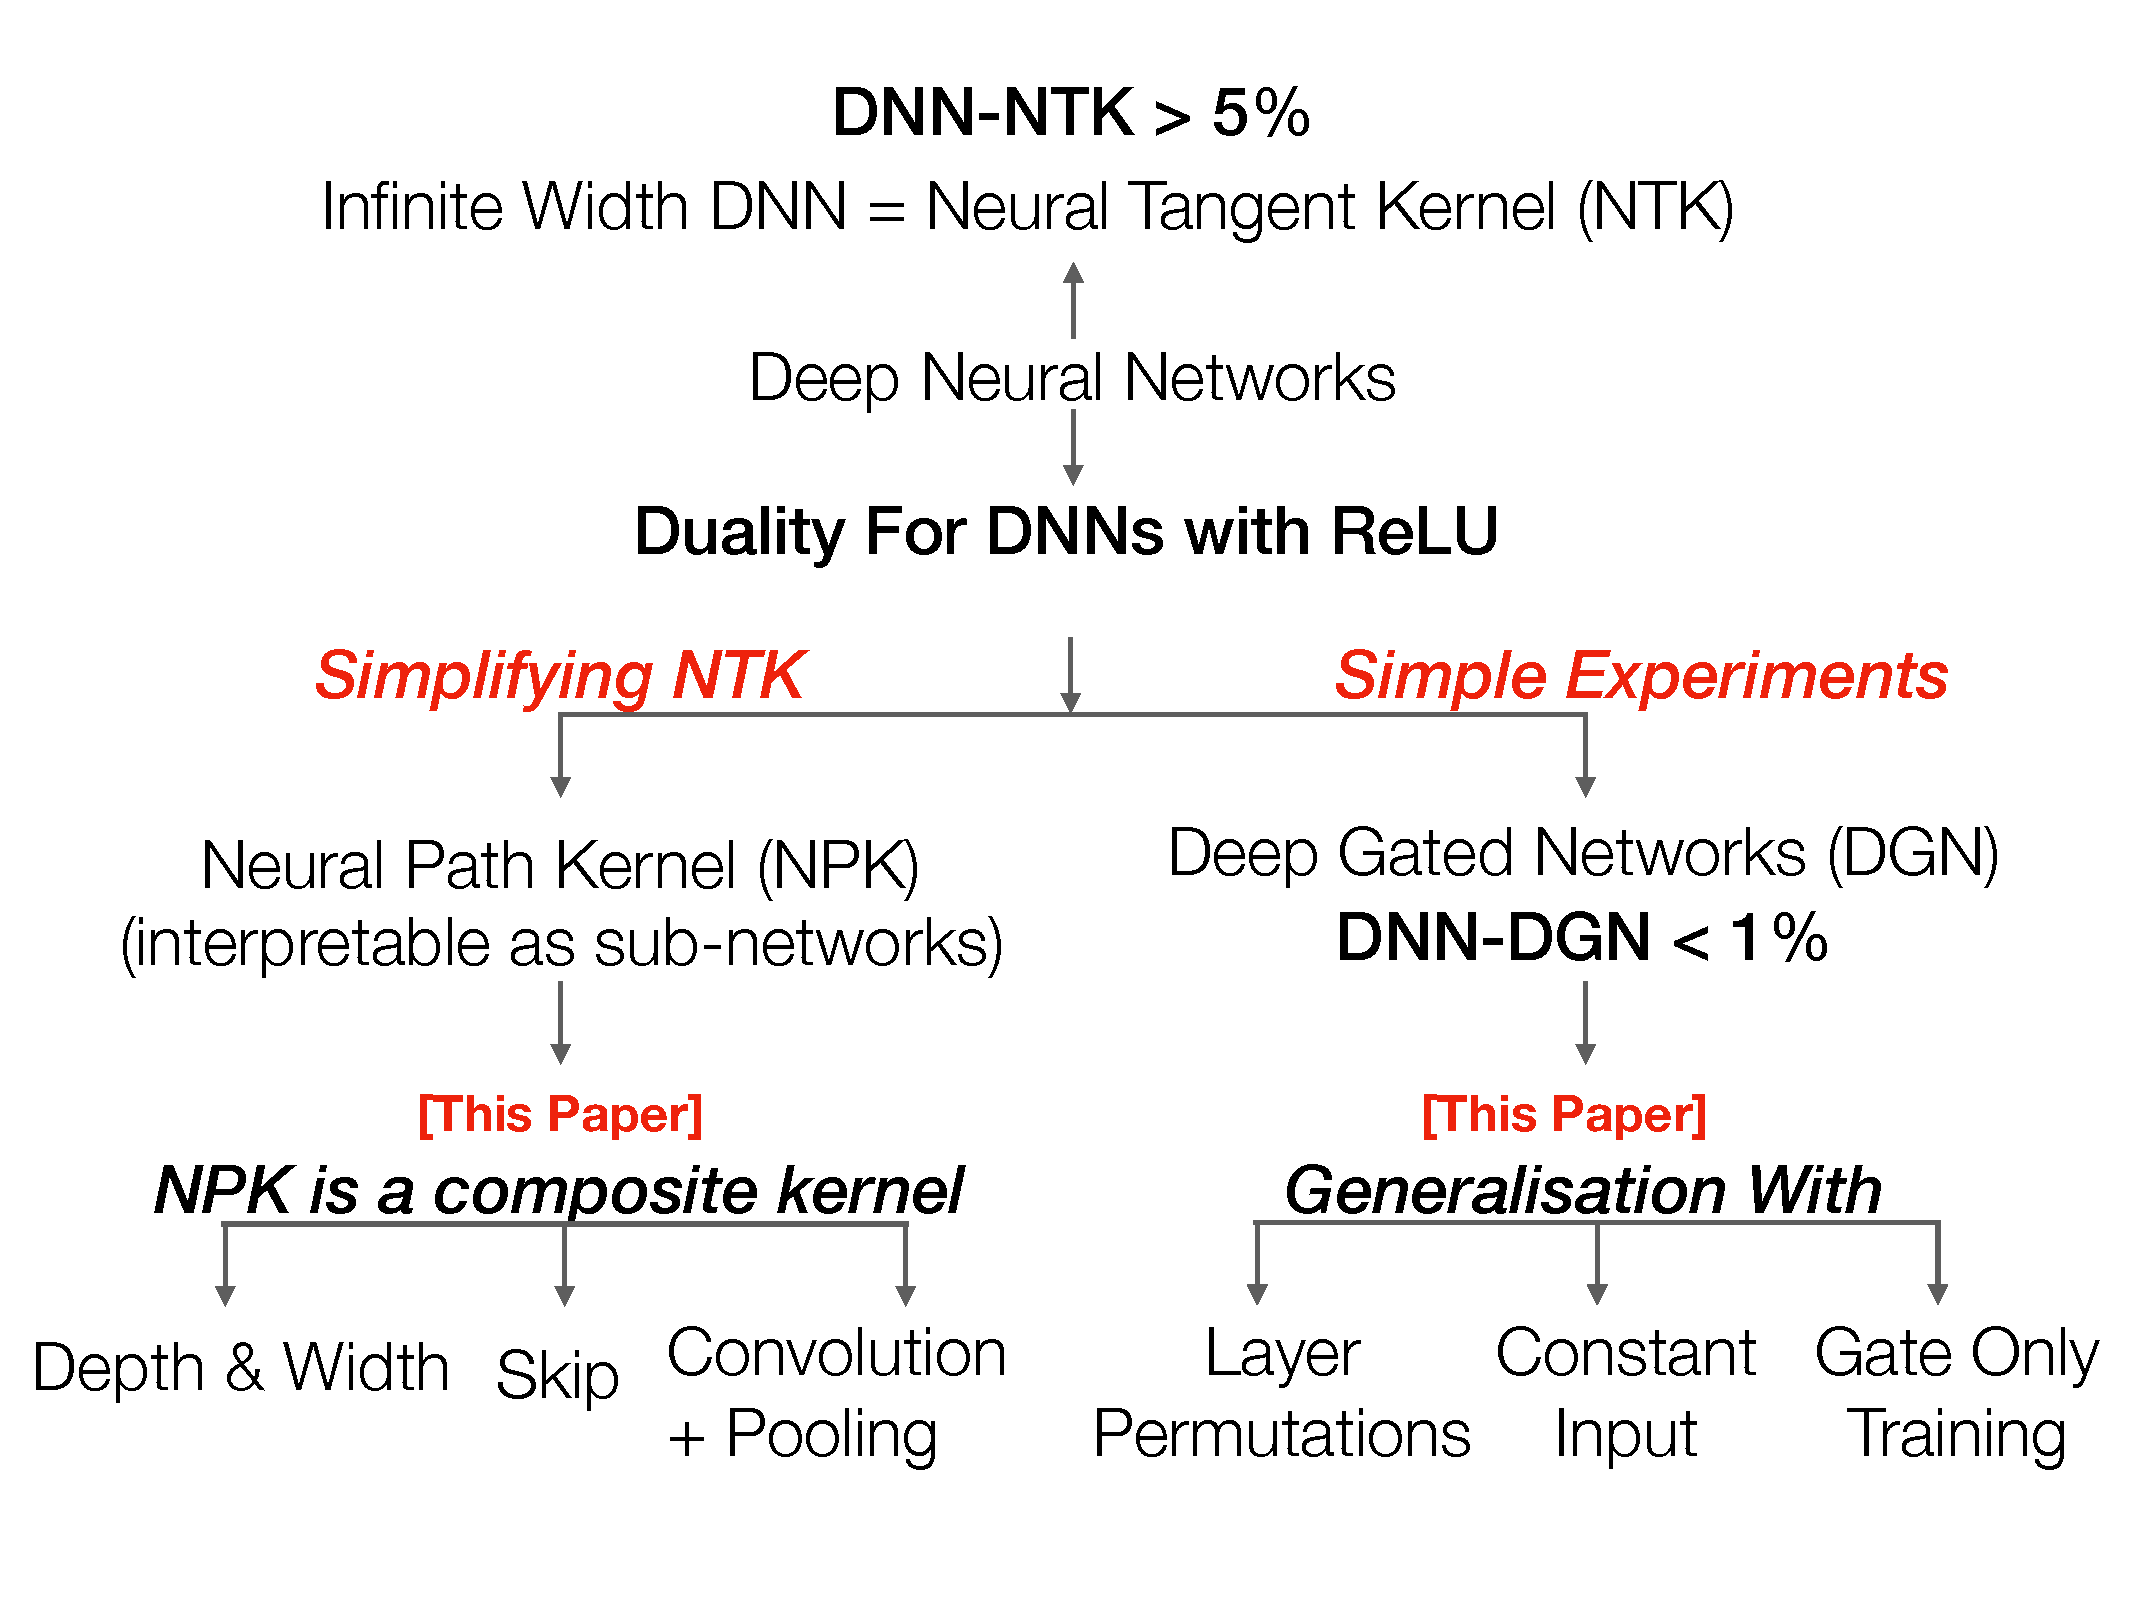
\includegraphics[scale=0.25]{figs/related.pdf}
}
\caption{This paper in relation to (i) NTK, (ii) Duality.}
\label{fig:related}
\end{figure}

\textbf{Duality and Simple Experiments:} In their recent work \cite{npk} proposed a dual approach to analyse DNNs with the rectified linear units (ReLUs). They exploited the special gating property of ReLU to devise a simple experimental setup called the deep gated network (DGN). In a DGN, the gates and the weights are held in separate networks as opposed to a DNN in which gates and weights are in the same network (see \Cref{fig:dgn}). They showed experimentally that:

\begin{figure}
\centering
\resizebox{\columnwidth}{!}{
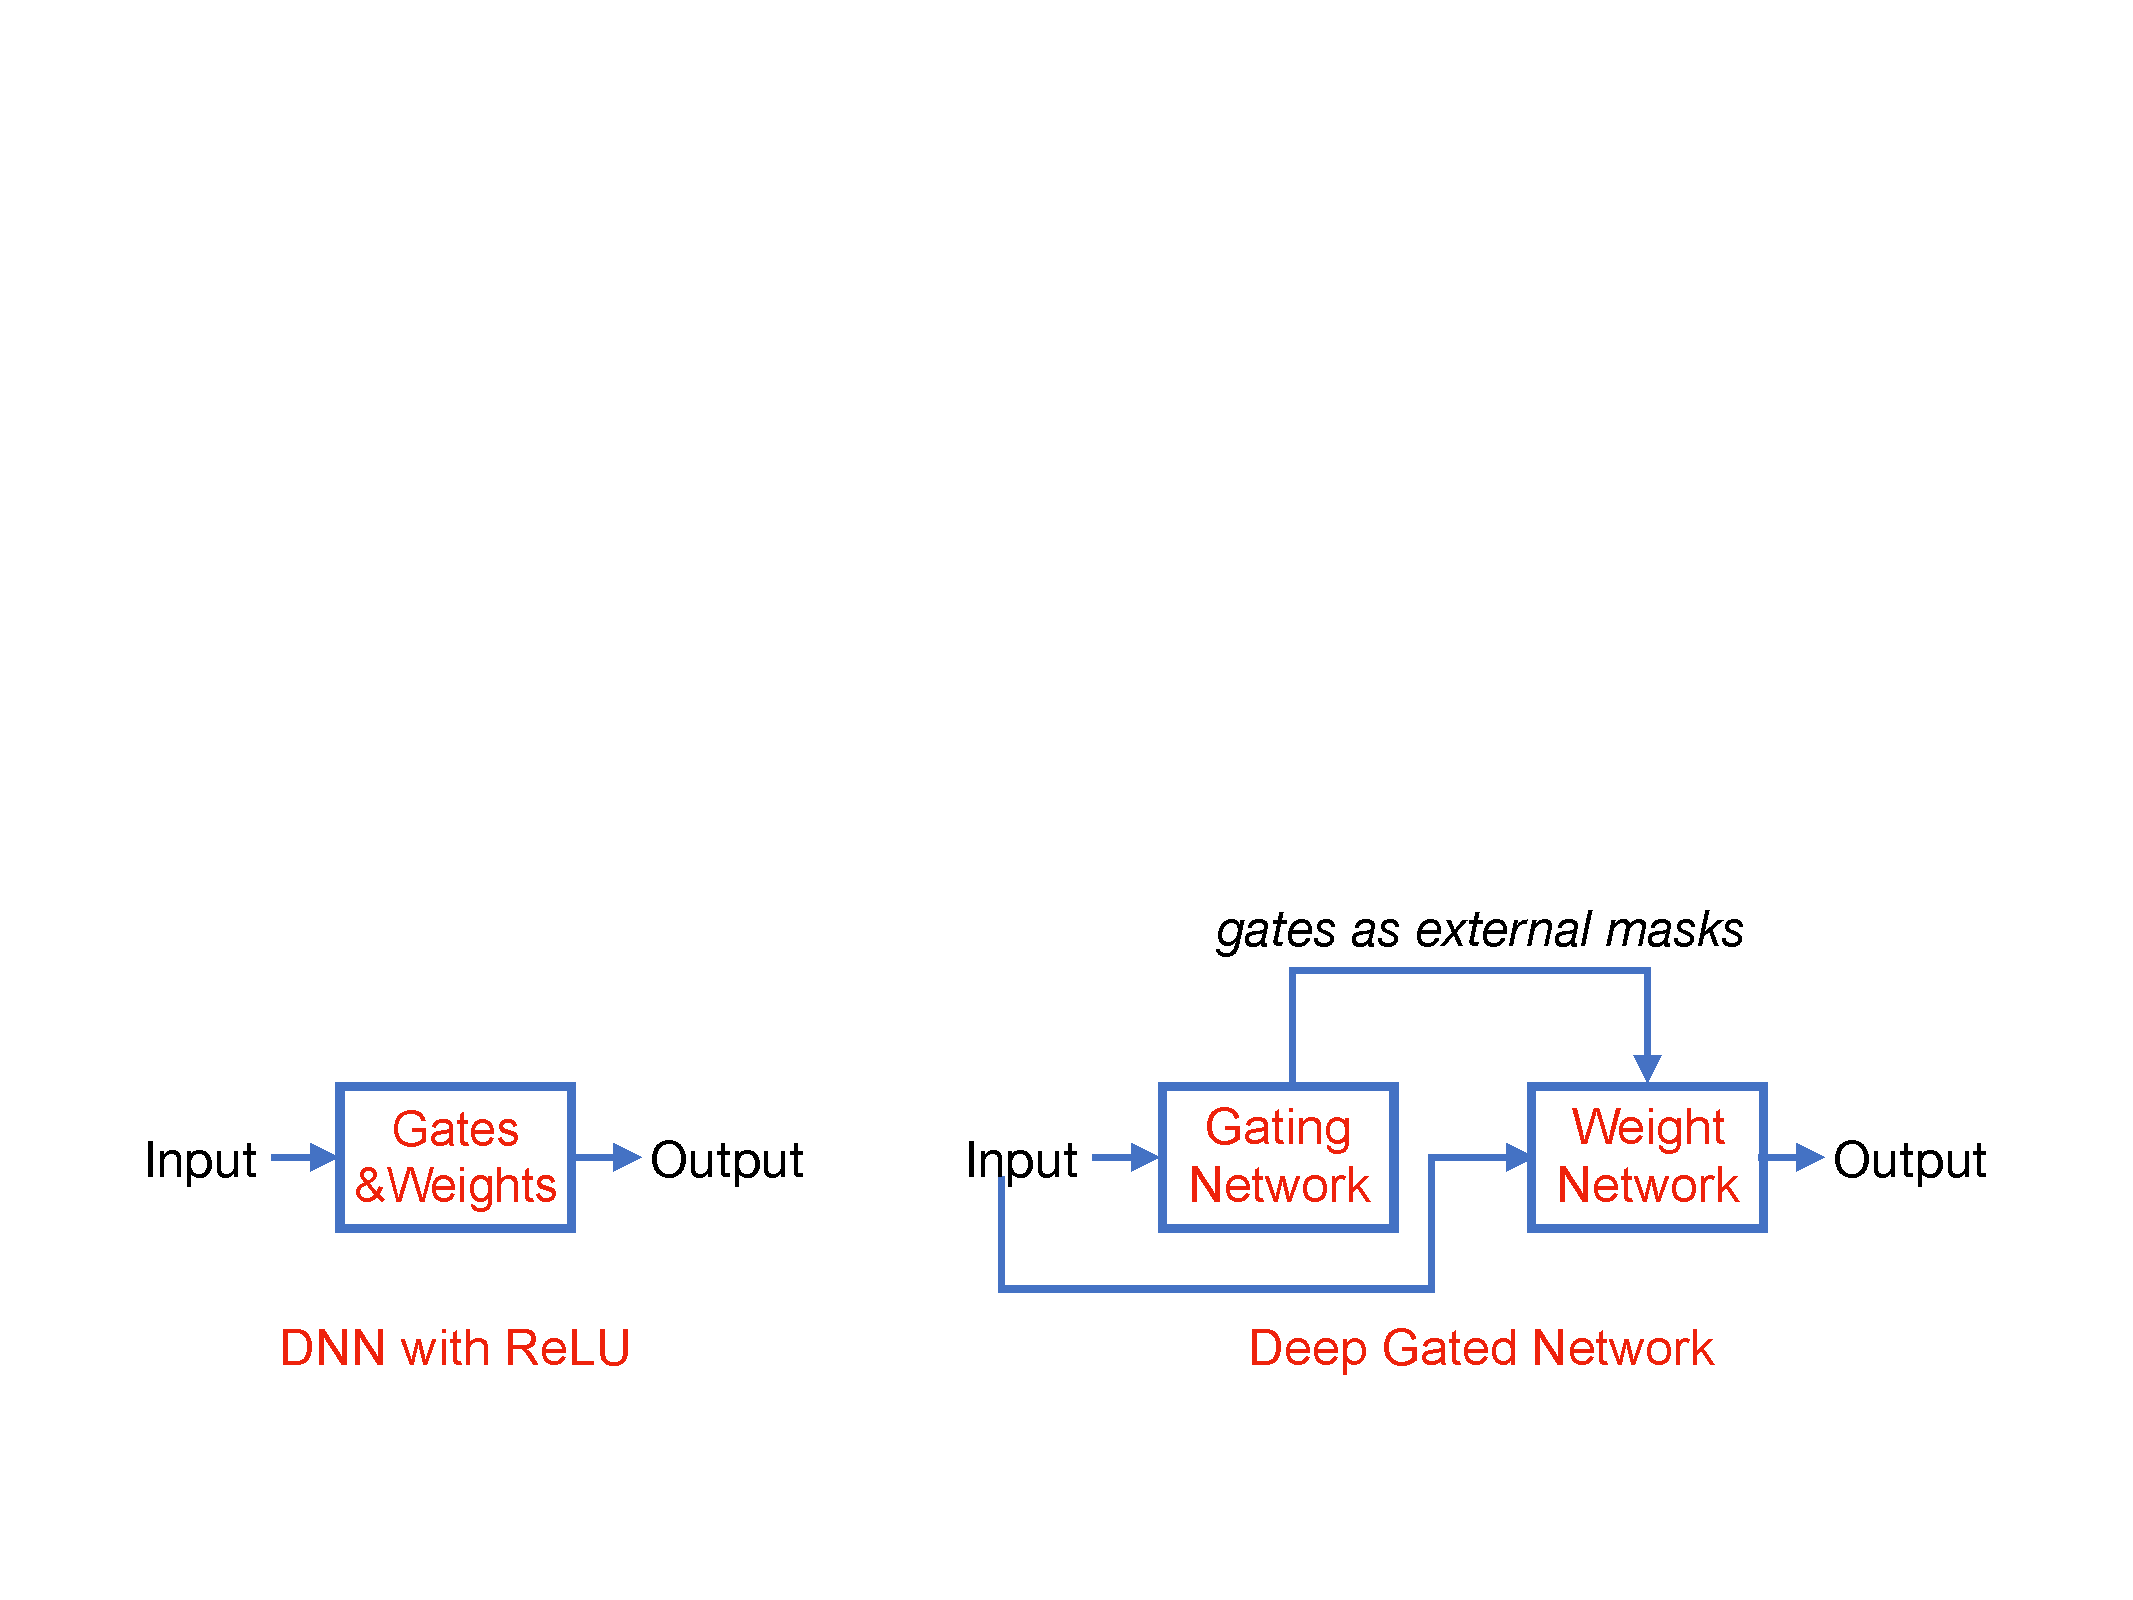
\includegraphics[scale=0.25]{figs/dnn-dgn.pdf}
}
\caption{DNN vs DGN.}
\label{fig:dgn}
\end{figure}
$1.$ \emph{Most information is in the gates:} By using just the gates of a pre-trained DNN (by letting it to be the gating network), the weight network can be trained to match the test performance (within $1\%$ ) of the DNN.

$2.$ \emph{Learning in gates} is the difference between finite width DNN and the infinite width NTK.  

\textbf{Duality simplifies NTK:} \cite{npk} showed that in a DGN, $\text{NTK}=\text{NTK}^{\text{fixed-gate}}+\text{NTK}^{\text{gate-learn}}$, where $\text{NTK}^{\text{fixed-gate}}$ is the kernel corresponding to learning of the weights with the gates fixed and $\text{NTK}^{\text{gate-learn}}$ is the kernel corresponding to learning of gates themselves. Further, $\text{NTK}^{\text{fixed-gate}}$ simplifies into a \emph{neural path kernel} (NPK), a kernel which is solely dependent on the information stored in the gates.



\subsection{Our Contributions}
The overall picture (see \Cref{tb:overall}) of duality together with NTK can be summarised as follows: (i) training and generalisation of infinite width DNNs is explain by the NTK \cite{arora2019exact,cao2019generalization}, (ii) the difference between finite width DNNs and infinite width DNNs is explained by learning in gates \cite{npk}, (iii) ReLU activation has a special role, i.e., they are gates, (iv) the primary role of the weights is to trigger the ReLU on/off. In this work we complete the picture by explaining the roles of width, depth, skip connections and convolutional layers with pooling.  The theoretical and experimental contributions are listed as under.

\FloatBarrier
\begin{figure}[h]
\centering
\resizebox{\columnwidth}{!}{
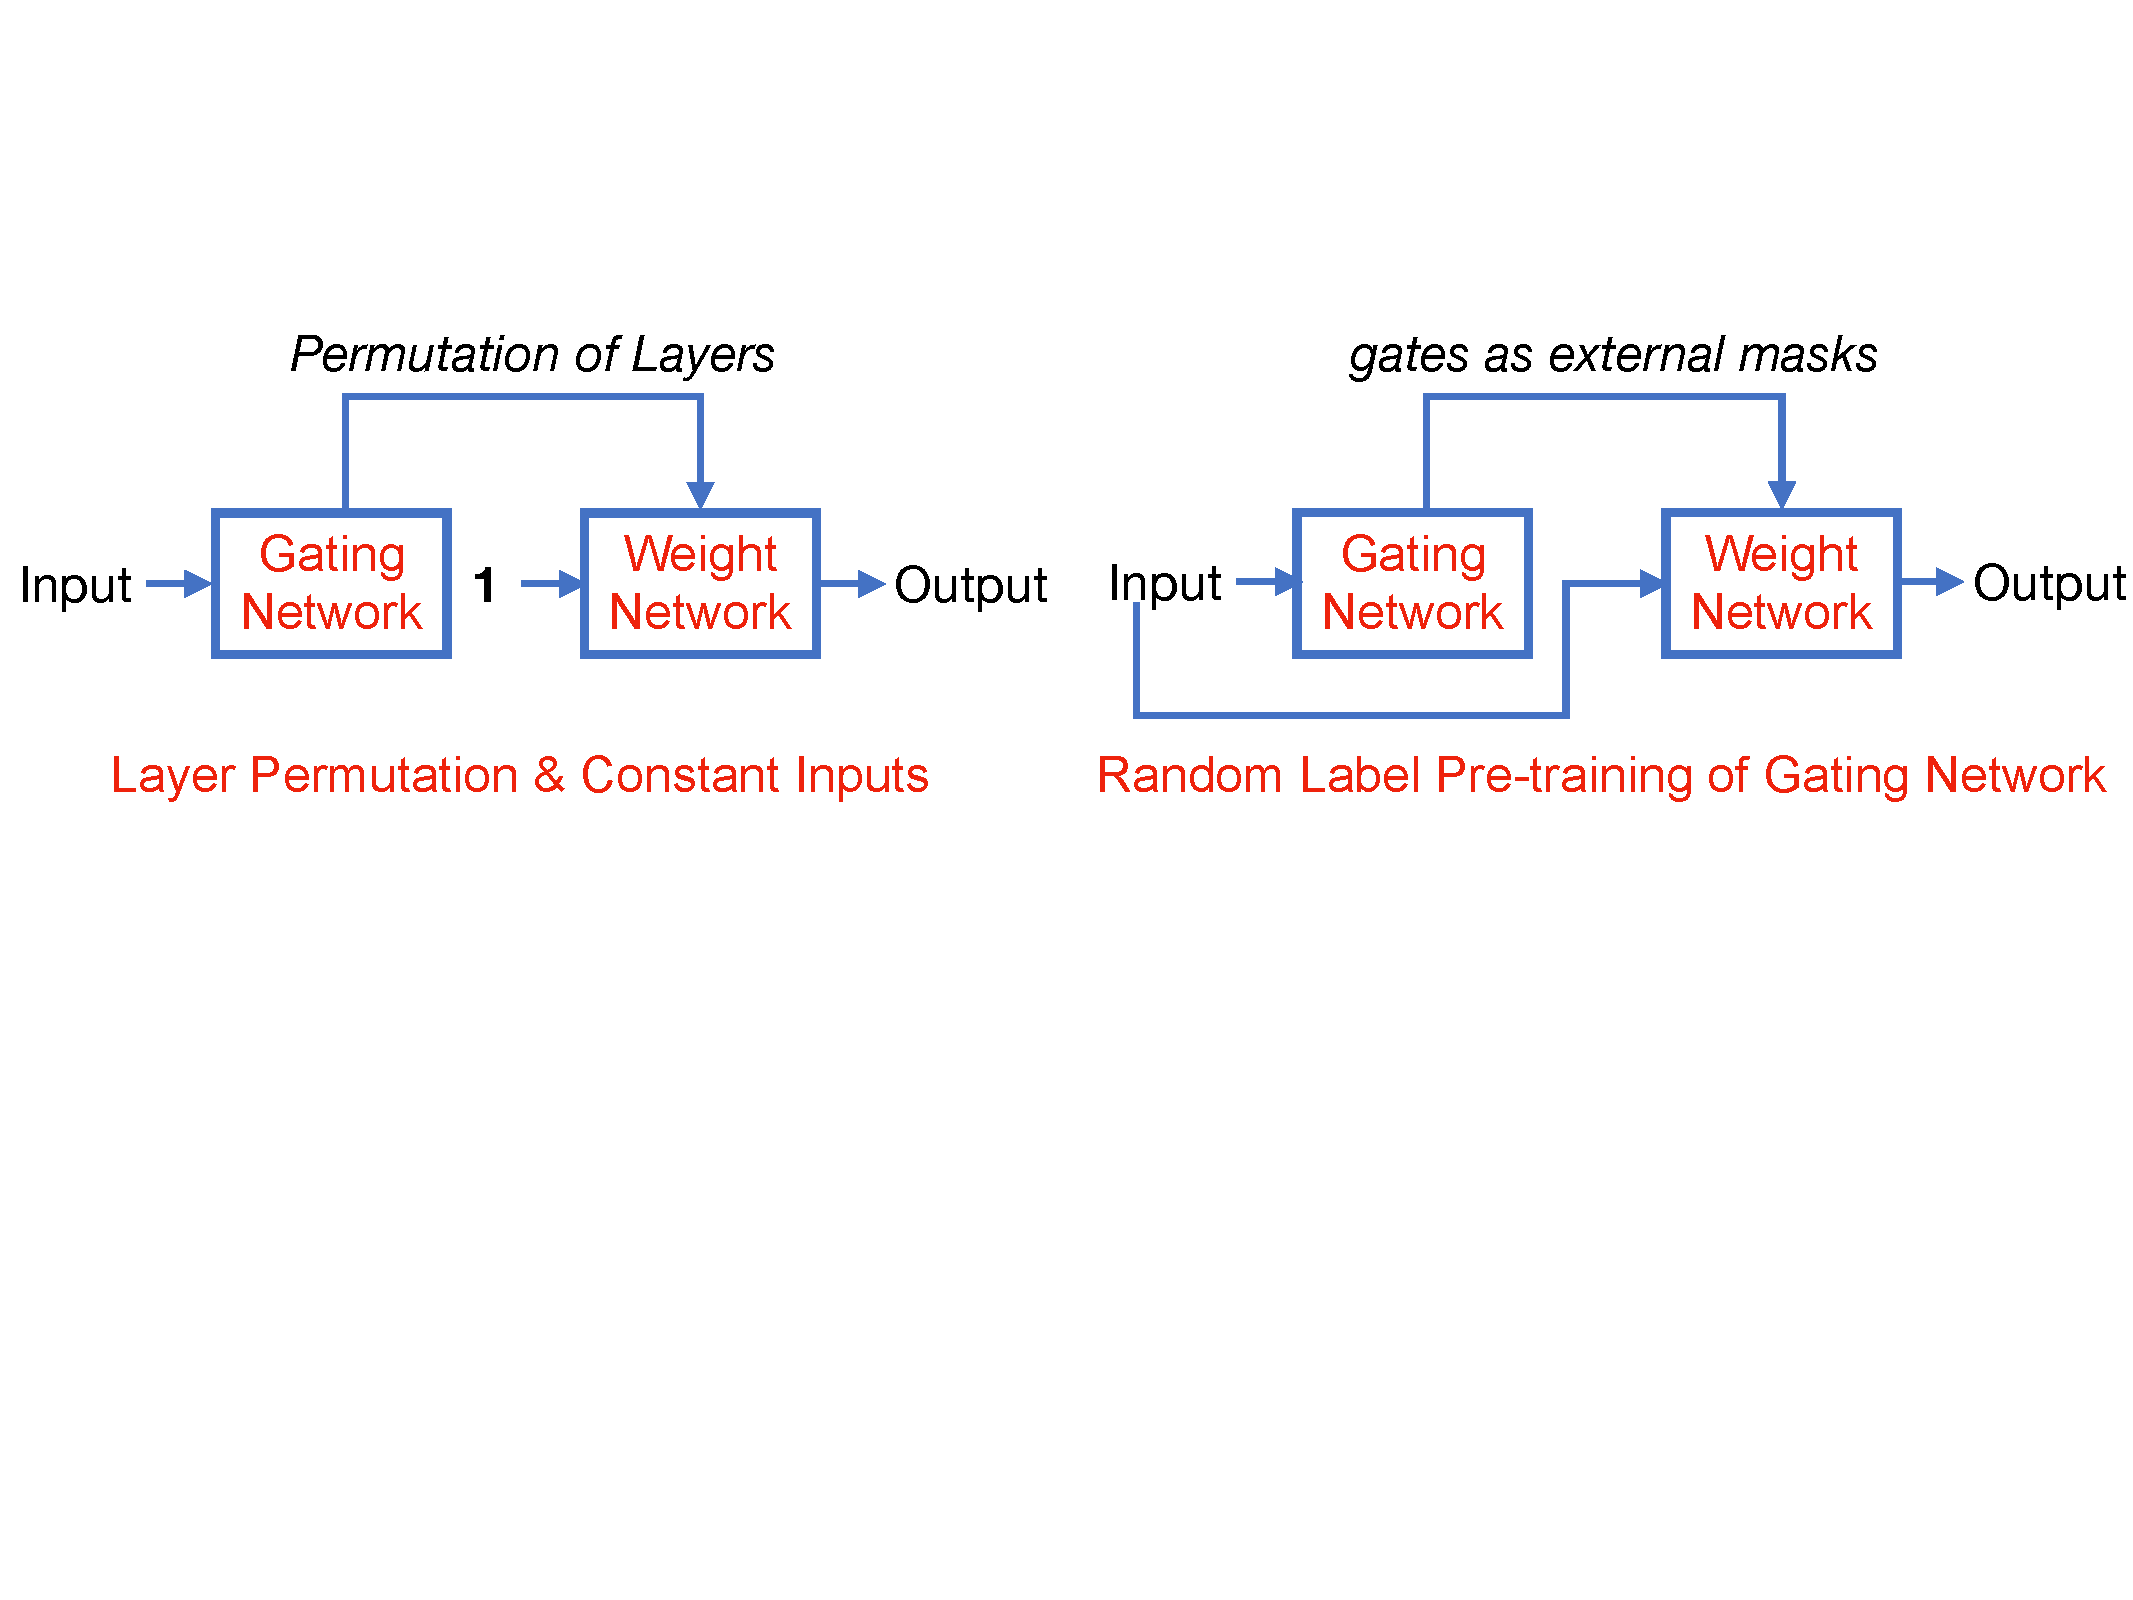
\includegraphics[scale=0.25]{figs/permute.pdf}
}
\end{figure}
\begin{comment}
\begin{table}
\centering
\begin{tabular}{p{1.75cm}p{2.25cm}p{2.25cm}p{0.01cm}}z
	     &\centering{Primal} 	& \centering{Dual+NTK}&\\\hline
Train, Gen. &\centering\ding{53}    & \centering{\ding{51}}& \\\hline
ReLU          &\centering{\ding{51}: yet another non-linearity} & \centering{\ding{51}: gates that are learnt}&\\\hline
Weights          &\centering{\ding{51}: linear part of a layer} & \centering{\ding{51}: triggers the gates}&\\\hline

\end{tabular}
\end{table}
\end{comment}

\begin{table}
\centering
\begin{tabular}{p{1.75cm}p{0.75cm}p{0.75cm}p{4cm}p{0.01cm}}
	     &\centering{Primal} &\centering NTK	& \centering{Dual+NTK [This Paper]}&\\
Train + Test &\centering\ding{53}  & \centering{\ding{51}},$*$  & \centering{\ding{51}},$**$& \\
ReLU          &\centering{\ding{53}} & \centering{\ding{53}} & \centering{\ding{51}}&\\
Weights          &\centering{\ding{53}} & \centering{\ding{53}}& \centering{\ding{51}}&\\
Width          &\centering{\ding{53}} & \centering{\ding{53}}& \centering{\ding{51}}&\\
Depth          &\centering{\ding{53}} & \centering{\ding{53}}& \centering{\ding{51}}&\\
Skip          &\centering{\ding{51}} & \centering{\ding{53}}& \centering{\ding{51}}&\\
Conv.+Pool          &\centering{\ding{51}} & \centering{\ding{53}}& \centering{\ding{51}}&\\
\end{tabular}
\caption{Overall picture. $*=$ does not explain difference between NTK and finite width DNN. $**=$ explains difference between NTK and finite width DNN}
\label{tb:overall}
\end{table}

\begin{comment}
\begin{table}
\begin{tabular}{ccccccccc}\hline
Primal & A & B & C& D & E& F & G & H\\ \hline
Primal & \ding{53} & \ding{53} & C & D & E& F & G & H\\ \hline
Kernel & A & B & C& D & E& F & G & H\\ \hline
Dual+NTK [This paper]& A & B & C& D & E& F & G & H\\ \hline
\end{tabular}
\end{table}
\end{comment}


\textbf{Theoretical Results:} We show that the NPK has a \emph{composite structure}, whose basic atomic units are the \emph{gates}. Specifically,

$\bullet$ \emph{Fully Connected DNN (FC-DNN):} In this case, the NPK involves a \emph{ Hadamard product of base kernels} structure. Here the most basic unit is the gate.  stacking ReLUs widthwise in a layer gives rise to a base kernel which measures the \emph{average} number of triggered ReLUs; stacking layers depthwise gives rise to a \emph{Hadamard product}. This result explains the roles of \emph{width and depth}.

$\bullet$ \emph{Residual networks with skip connections:} In this case, the NPK involves a  \emph{ sum of Hadamard product of base kernels} structure. This result explains the role of skip connections.

$\bullet$ \emph{Convolutional layers with pooling:} In this case, the NPK  has a  \emph{rotational invariant} structure. This result explains the role of convolutions and pooling from a kernel standpoint.

\textbf{Experimental Results:} We collect more supporting evidence for the claim \emph{most information is in the gates}. In particular, our results show that the standard view that hidden layer outputs is a red-herring and the actual feature learning happens in the gates. To bolster our case, we build combinatorially many models by (i) permuting the order of the layers when we apply them as external masks and providing a tensor with all entries $1$ instead of the input image. 

\textbf{Message:} The primal \emph{layer-by-layer} and the dual \emph{path-by-path} views of computations complement each other. While the primal computations is used in \emph{actual} training and our results suggest that dual view is quite for understanding. 

\begin{comment}
 We consider deep neural networks (DNNs) with \emph{rectified linear units} (ReLUs). For such DNNs, we propose a \emph{pedagogical nugget} ``simple theorems, simple experiments" \cite{Aliresponse} by combining \emph{neural tangent kernel} (NTK) and \emph{dual view}. Our aim is to explain training, generalisation, roles of weights/activation/width/depth/convolutions with pooling/skip connections. Training and generalisation of infinite width DNN 


In this paper, we make two major contributions using the lens of dual view. Firstly, we show that the NPK has a \emph{compositional} structure. The results are listed below.

$\bullet$ \emph{Fully Connected DNN (FC-DNN):} In this case, the NPK involves a \emph{ Hadamard product of base kernels} structure. Here the most basic unit is the gate.  stacking ReLUs widthwise in a layer gives rise to a base kernel which measures the \emph{average} number of triggered ReLUs; stacking layers depthwise gives rise to a \emph{Hadamard product}. This result also explains the roles of \emph{width and depth}.

$\bullet$ \emph{Residual networks with skip connections:} In this case, the NPK involves a  \emph{ sum of Hadamard product of base kernels} structure.

$\bullet$ \emph{Convolutional layers with pooling:} In this case, the NPK  has a  \emph{rotational invariant} structure.

Our second major contribution is an ablation study to argue that the standard view that hidden layer outputs is a red-herring and the actual feature learning happens in the gates. To bolster our case, we build combinatorially many models by,

1. permuting the order of the layers when we apply them as external masks,

2. providing a tensor with all entries $1$ instead of the input image. 

We observe in our experiments that the performance is robust to such combinatorial variations.

We also show experimentally how training with random labels affects the gates, and experimentally verify how skip connections improve the conditioning of the underlying NTK.
\end{comment}
\subsection{Organisation}
\subsection{Notation}
\section{Neural Tangent Kernel}
%In this section, we define the neural tangent kernel (NTK) (see \Cref{def:ntk}) and briefly discuss its connection to training and generalisation of DNNs, and limitation of the NTK based approach to understand DNNs.
Several works \cite{ntk,fcgp,convgp,arora2019exact,arora} have been successful in connecting the training and generalisation of DNNs to kernel methods. An important kernel associated with a DNN is the so called \emph{Neural Tangent Kernel (NTK)} defined as follows.
\begin{definition}\label{def:ntk}
 For input examples $x,x'\in\R^{\din}$, the neural tangent kernel (NTK), denoted by $K_{\Theta}(x,x')$ is defined as:
\centerline{$
K_{\Theta}(x,x') = \langle\nabla_{\Theta} \hat{y}_{\Theta}(x), \nabla_{\Theta} \hat{y}_{\Theta}(x') \rangle
$}
\end{definition}
The NTK is related to the \emph{full training}\footnote{In contrast to the \emph{lazy training} regime, wherein, only the last layer weights of the DNN are trained (while other layer weights are \emph{frozen}, i.e., kept fixed during training). Kernel associated with the \emph{lazy regime} is known as the \emph{Conjugate Kernel} (CK). Since the NTK  \cite{arora2019exact} is better than the CK \cite{convgp} both as an approximation and as a standalone kernel method, we focus only on the NTK.}  regime wherein, all the weights are trained using gradient descent. The following result shows how the NTK naturally arises in DNNs trained by gradient descent.
\begin{proposition}[\textbf{Lemma 3.1} by \citet{arora2019exact}]\label{prop:basic}
Let $e_{\Theta}=\left(\hat{y}_{\Theta}(x_s)-y_s,s\in[n]\right)\in\R^n$ be the error in prediction. Let $\dot{\Theta}_t=-\nabla_{\Theta}L_{\Theta_t}$ denote gradient descent  with infinitesimally small step-size to minimise the  squared loss $L(\Theta)=\frac{1}{2}\norm{e_{\Theta}}_2^2$. It follows that the dynamics of the error term (during gradient descent) can be written as:\\ \centerline{$\dot{e}_{\Theta_t}=-K_{\Theta_t} e_{\Theta_t}$.} 
\end{proposition}
The NTK has appeared in various prior works \cite{ntk,dudnn,arora2019exact,cao2019generalization}. In what follows, for the sake of brevity, we mainly refer to the results by \citet{arora2019exact}. 

\textbf{Key Points:} \citet{arora2019exact} showed that under appropriately randomised initialisation, as the width goes to infinity, $K_{\Theta_0}\ra K_*$, and $K_{\Theta_t}\approx K_{\Theta_0}$, where $K_*$ is the limiting (deterministic) NTK matrix. The main result is that an infinite width DNN trained using GD is equivalent to a kernel method with $K_*$.  They also proposed a pure kernel method  called the convolutional NTK (CNTK), which is the limiting NTK matrix  of an infinite width convolutional neural network (CNN). On CIFAR-10, CNTK  performs better than prior kernel methods by $10\%$. Despite the success of NTK as a pure kernel method, there are some issues.  Firstly, standard CNN still outperforms its corresponding CNTK by $5-6\%$. Secondly, since the infinite limit NTK `$K_*$' is a fixed deterministic matrix, there is no feature learning, whereas feature learning is believed to be the unique differentiator of DNNs from other the machine learning methods. Thus, NTK does not fully explain finite width DNNs. 

\section{Duality: DNNs are both layers and paths}
In this section we explain the notion of duality in DNNs with ReLUs. 
\subsection{Gating property of ReLU}
A special property of ReLU is that it is also a gate which either blocks (i.e., multiplies by $0$) or allows (i.e., multiplies by $1$) its pre-activation input. 
\FloatBarrier
\begin{figure}[H]
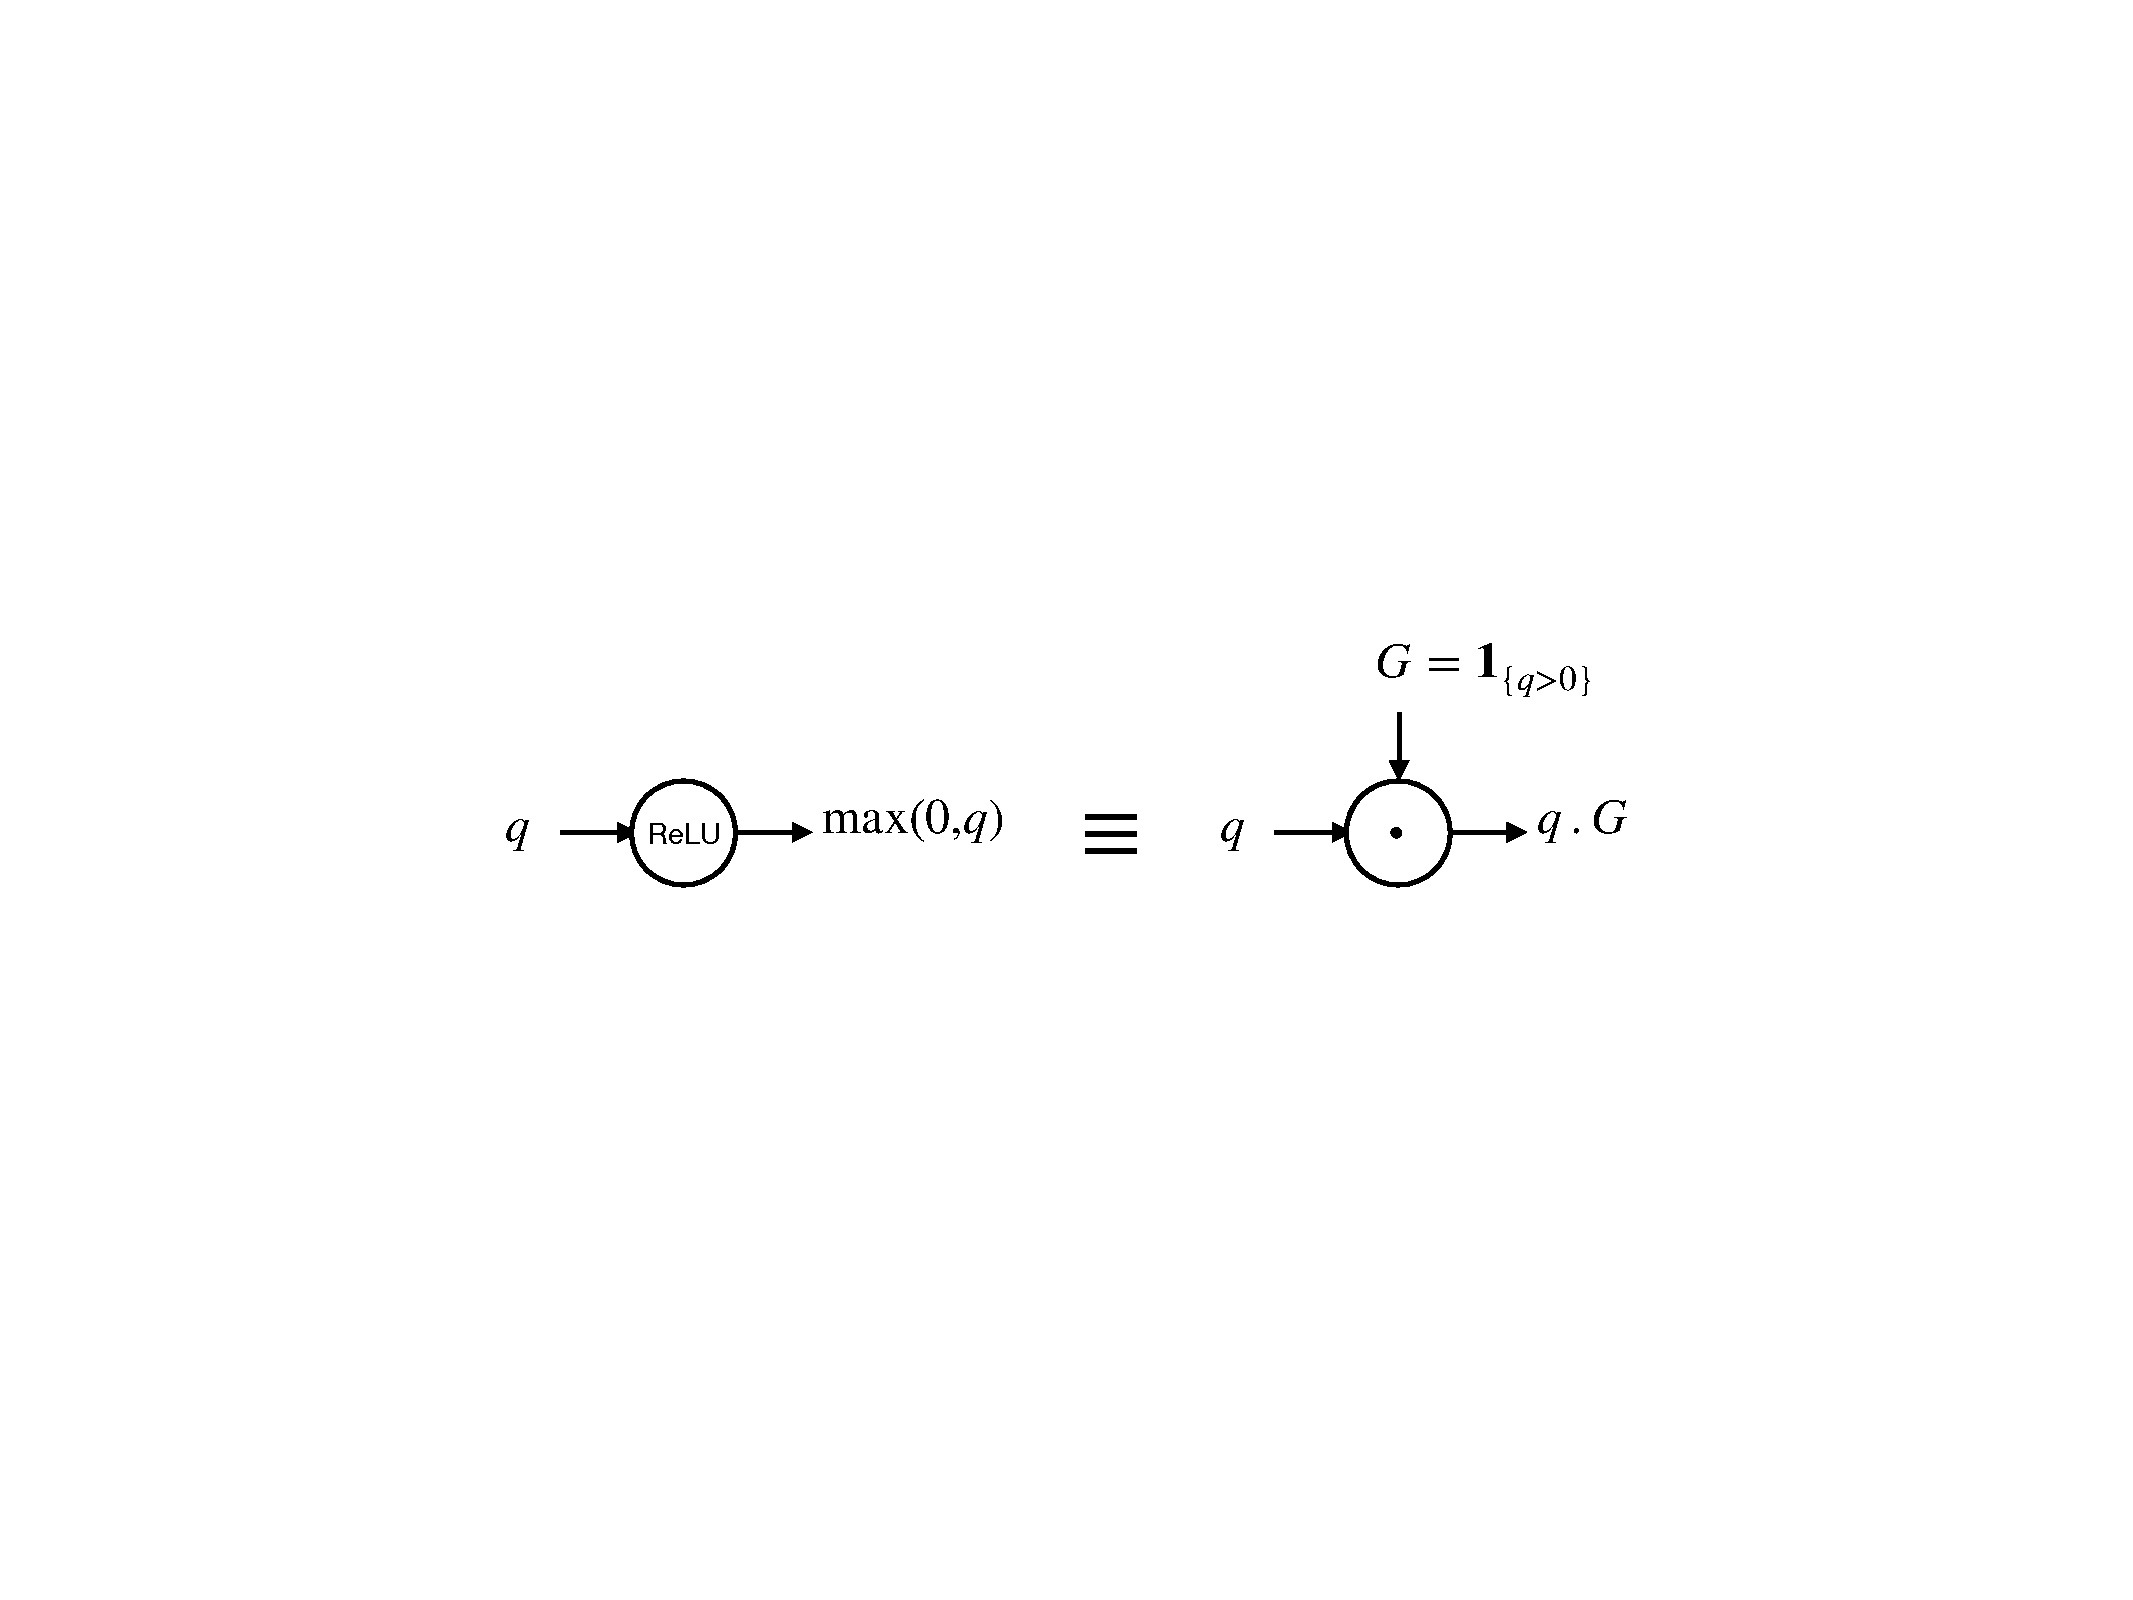
\includegraphics[scale=0.4]{figs/gating.pdf}
\end{figure}
\subsection{Output Expression: Primal vs Dual}
A consequence of the gating property is \emph{duality}: DNNs are layers (primal view) as well as paths (dual view). The difference between the primal and the dual way of expressing the network output can be seen in \Cref{tb:primal-dual}
\FloatBarrier
\begin{table}[H]
\resizebox{\columnwidth}{!}{
\begin{tabular}{|c|c|}\hline
Primal & $\hat{y}_{\Theta}(x)=\Theta(d)\text{ReLU}\Bigg(\Theta(d-1)\text{ReLU}\Big(\cdots\text{ReLU}\big(\Theta(1)x\big)\Big)\Bigg)$ \\\hline
Dual  & $\hat{y}_{\Theta}(x)=\sum_{\text{path}}\text{individual path contribution}$ (see \Cref{prop:zero})\\\hline
\end{tabular}
}
\caption{$\Theta(l),l=1,\ldots,d$ is the weight of layer $l$.}
\label{tb:primal-dual}
\end{table}

\subsection{Path, Neural Path Feature and Value}
\FloatBarrier
\begin{figure}[h]
\centering
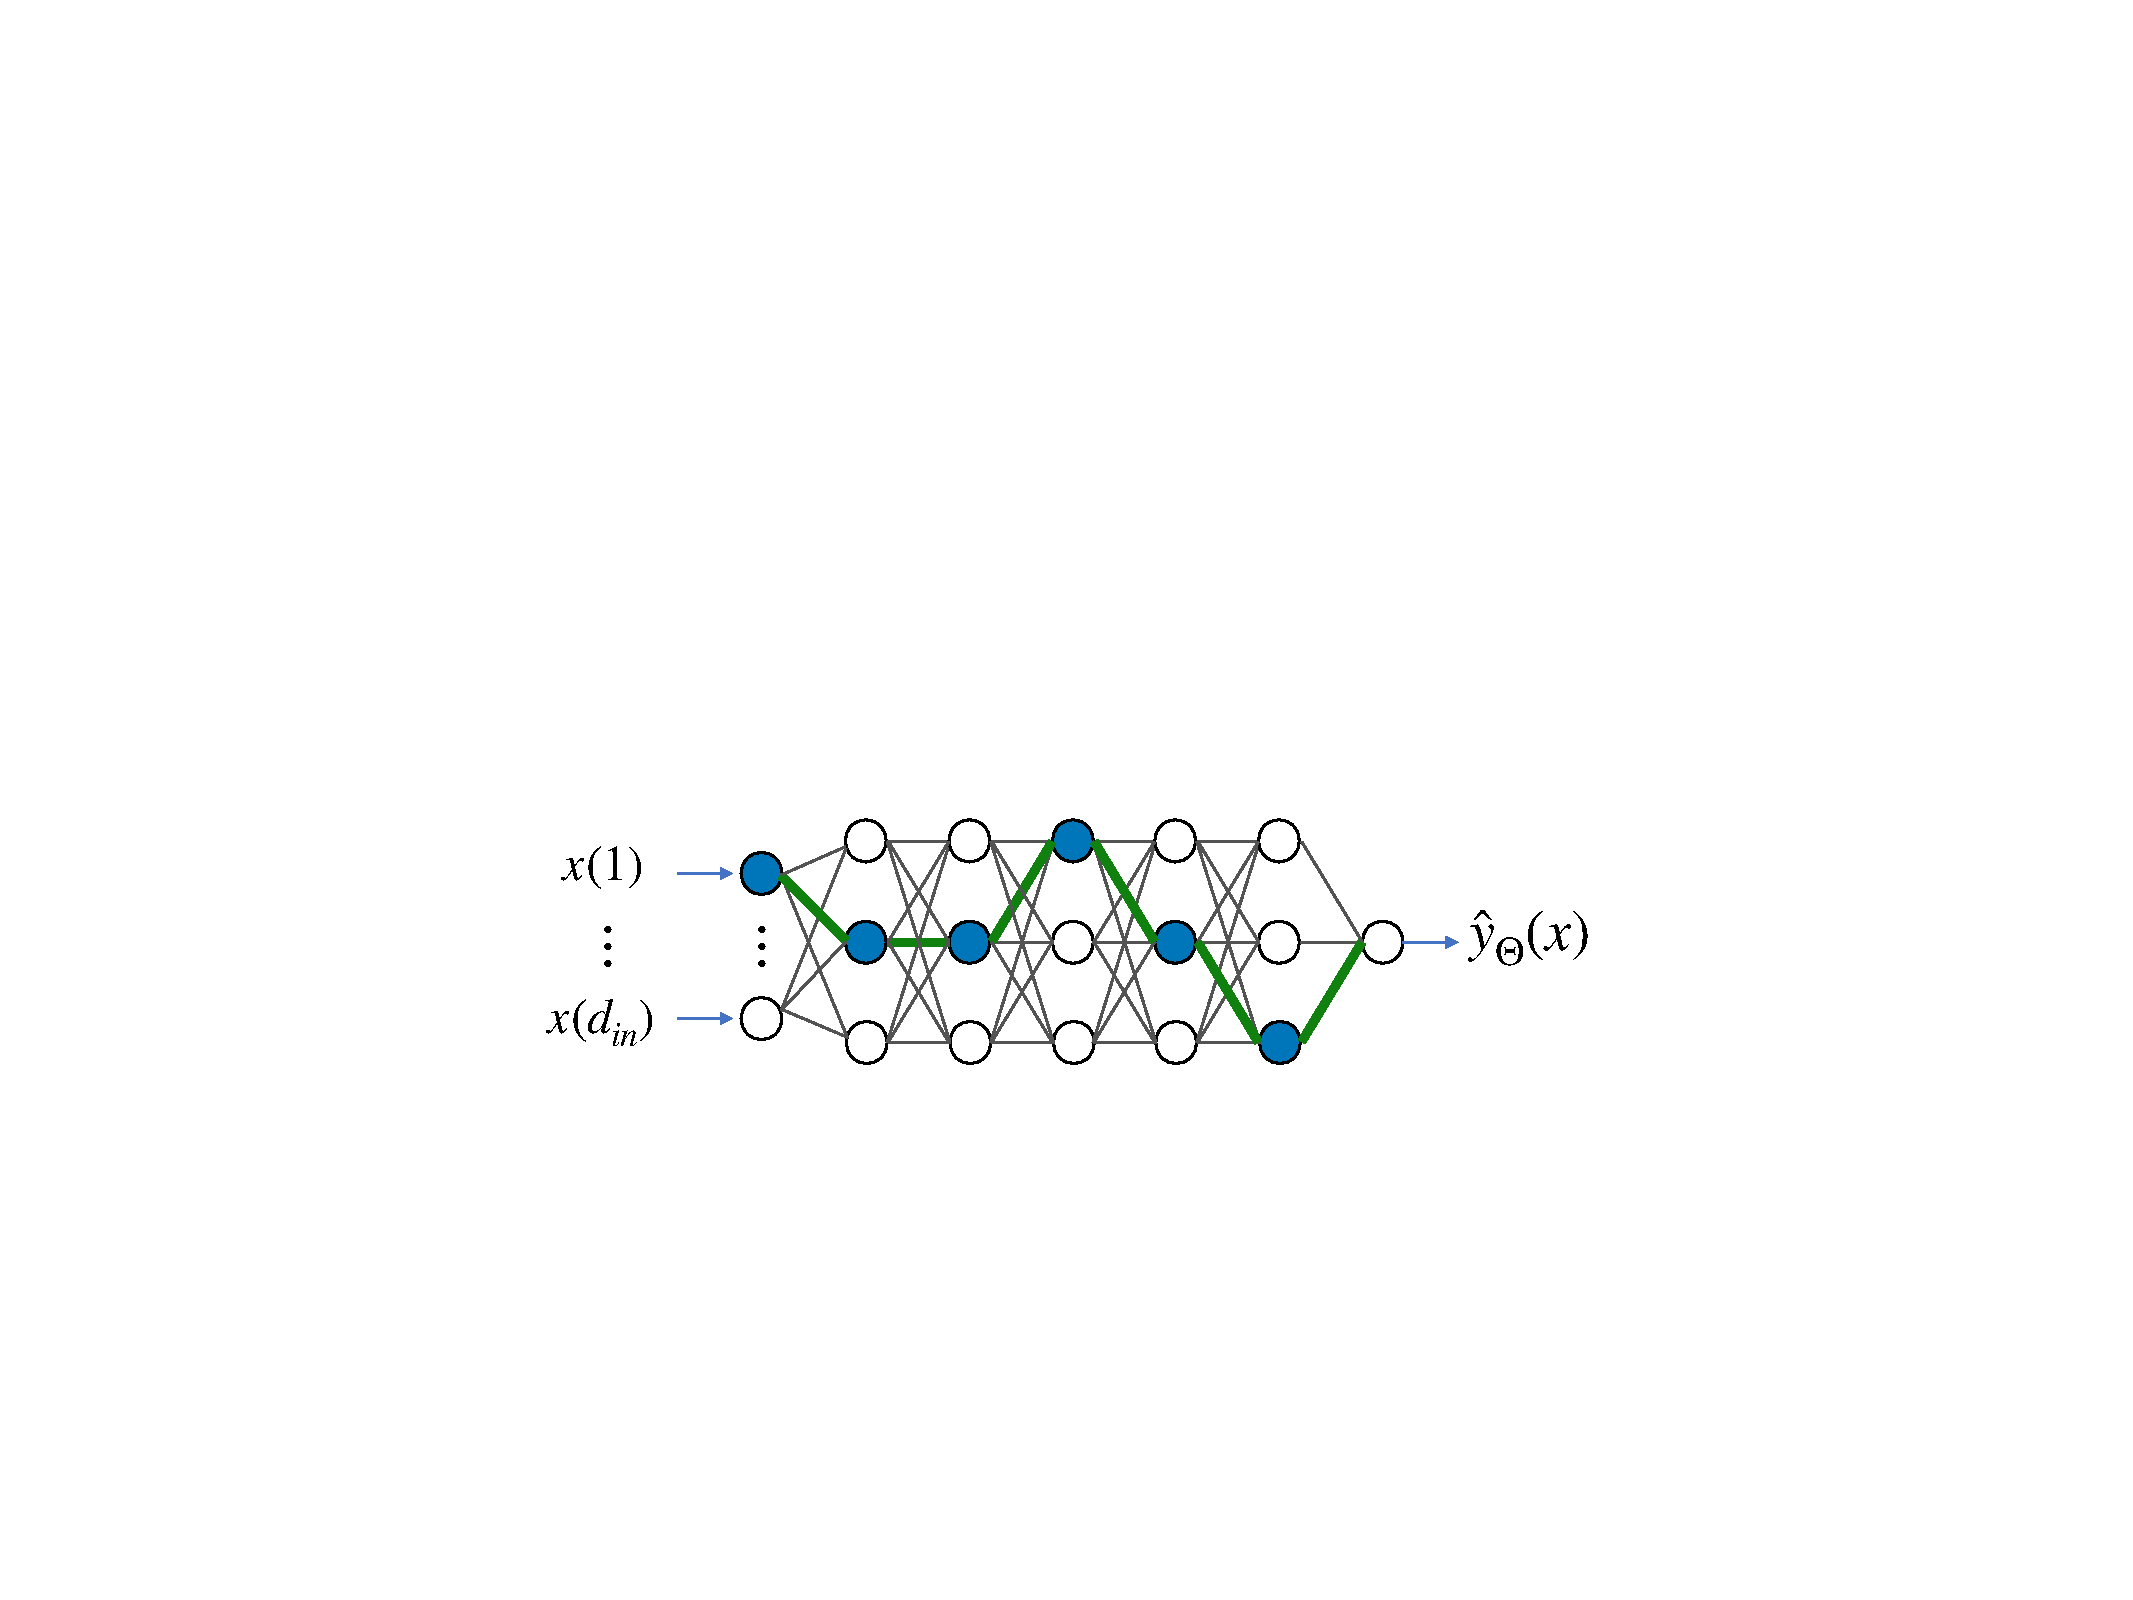
\includegraphics[scale=0.32]{figs/paths.pdf}
\end{figure}
A path starts from an input node, passes through exactly one weight and one hidden node in each layer and ends at the output node. We have a total of $P=\din w^{(d-1)}$ paths. We assume that there is a natural enumeration of the paths, and denote the set of all paths by $[P]$.
\begin{definition}\label{def:nps} Let $x\in\R^{\din}$ be the input to the DNN. For this input, 

(i)  $A_{\Theta}(x,p)\stackrel{def}{=}\Pi_{l=1}^{d-1} G_{x,\Theta}(l,p)$ is the activity of a path.

(ii)  $\phi_{x,\Theta}\stackrel{def}=\left(x(\I_0(p))A_{\Theta}(x,p) ,p\in[P]\right)\in\R^P$ is the {neural path feature} (NPF).

(iii)  $v_{\Theta}\stackrel{def}=\left(\Pi_{l=1}^d \theta(l,p),p\in[P]\right)\in\R^P$ is the {neural path value} (NPV).
\end{definition}
\begin{proposition}\label{prop:zero}  The output of the network can be written as an inner product of the NPF and NPV, i.e., 
$\hat{y}_{\Theta}(x)=\ip{\phi_{x,\Theta},v_{\Theta}}=\sum_{p\in [P]}x(\I_0(p))A_{\Theta}(x,p)v_{\Theta}(p)$.
\end{proposition}

\section{Duality + NTK: First Step}


\begin{comment}
\subsection{Active Sub-Networks}
\FloatBarrier
\begin{figure}[H]
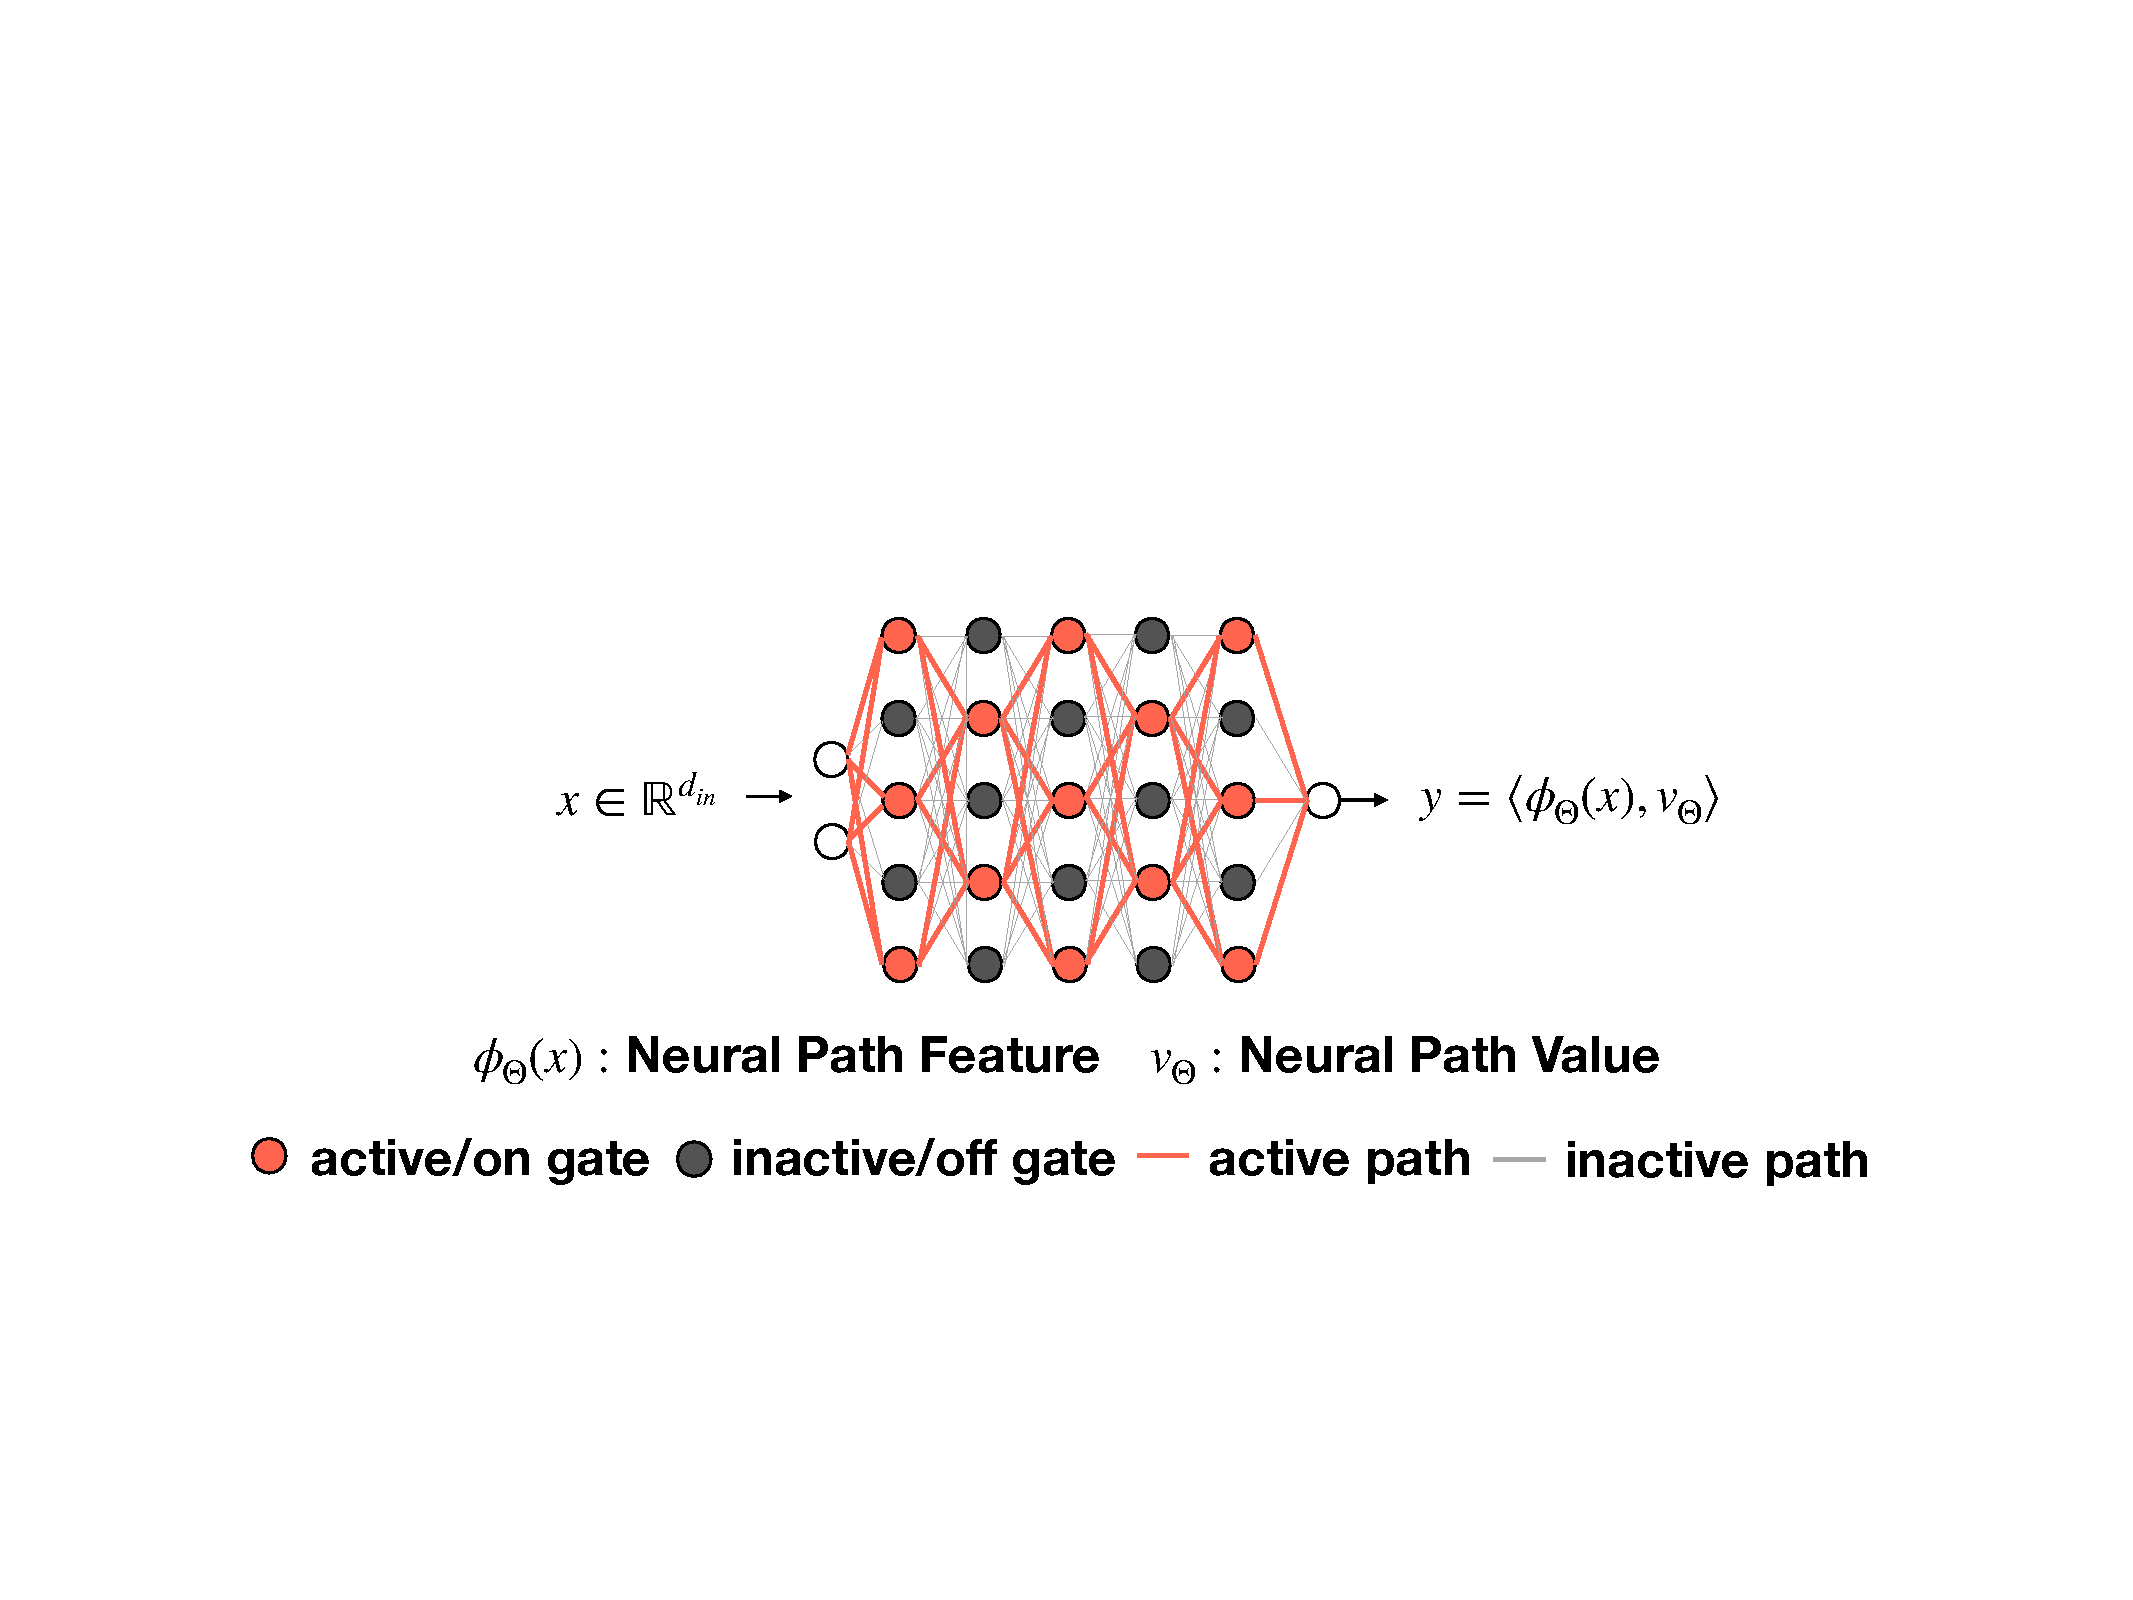
\includegraphics[scale=0.25]{figs/step1.pdf}
\end{figure}




\cite{npk} used duality to separate the gates as masks from the weights and argued (via experiments and theory) that \emph{gates of a DNN alone is enough to obtain power insights}. The key experimental and theoretical results are summarised in the next two points.

1. \textbf{Experimental:} Using a deep gate network to decouple the gates as masks from the weights, it was shown that  (i) gates are learnt during training, (ii) learnt gates generalise better, (iii) most information is in the gates, i.e., with learnt gates as masks the weights can be reset and retrained without significant loss in test accuracy (iv) learning in gates is the reason why finite width DNNs perform better than infinite width NTK.


2.  \textbf{Theoretical:}  When the gates are decoupled from weights, the NTK is a summation of two kernels, i.e., NTK = $\text{NTK}^{\text{fixed-gate}}+ \text{NTK}^\text{gate-learning}$, where $\text{NTK}^{\text{fixed-gate}}$ is the kernel that corresponds to learning the wights keeping the gates fixed and $\text{NTK}^\text{gate-learning}$ is the kernel corresponds to learning of the gates themselves. Main theorem shows that the $\text{NTK}^{\text{fixed-gate}}$ simplifies into a \emph{neural path kernel} (NPK), which measures the similarity of a given pair of input examples in terms of the size of sub-network that is active\footnote{Active sub-network comprises of the gates which are \emph{on} (i.e., $1$) and the weights connecting such gates.} simultaneously for both the input examples.  


Since we will be using the dual view, we now provide a brief summary of the same.
\end{comment}
\begin{comment}
Rewriting everything in terms of gates.
Simple Theory: Kernel depends on only gates. NTK = NPK

Simple Experiments: Instead of designing another kernel method based on NPK we have 2 choices i) design another kernel ii) use the observation to more simple experiments. that NPK Keep experimenting with various gating patterns.


\subsection{Neural Path Kernel and Correlation of Sub-Networks}
\begin{definition}\label{def:lambda}
 For input examples $s,s'\in[n]$, define $Act_{\Theta}(s,s')\stackrel{def}=\{p\in[P]\colon A_{\Theta}(x_s,p)= A_{\Theta}(x_{s'},p)=1\}$ to be the set of `active' paths for both $s,s'$  and $\Lambda_{\Theta}(s,s')\stackrel{def}=\frac{|Act_{\Theta}(s,s')|}{\din}$.
\end{definition}
\textbf{Remark:} Owing to the symmetry of a DNN, the same number of active paths start from any fixed input node. In \Cref{def:lambda}, $\Lambda_{\Theta}$ measures the size of the active sub-network as the total number of active paths starting from any fixed input node. For examples $s,s'\in[n],s\neq s'$, $\Lambda_{\Theta}(s,s)$ is equal to the size of the sub-network active for $s$, and $\Lambda_{\Theta}(s,s')$ is equal to the size of the sub-network active for both $s$ and $s'$. For an illustration of NPFs and $\Lambda$ please see \Cref{fig:npkexample}.
\begin{lemma}\label{lm:npk}
Let $H_{\Theta}\in\R^{n\times n}$ be the NPK matrix, whose entries are given by $H_{\Theta}(s,s')\stackrel{def}{=}\ip{\phi_{x_s,\Theta},\phi_{x_{s'},\Theta}},s,s'\in[n]$. Let $\Sigma\in\R^{n\times n}$ be the input Gram matrix with entires $\Sigma(s,s')=\ip{x_s,x_{s'}},s,s'\in[n]$. It follows that $H_{\Theta}= \Sigma\odot\Lambda_{\Theta}$, where $\odot$ is  the Hadamard product.
\end{lemma}


\subsection{Deep Gated Networks: Gates are External Masks}


\subsection{NTK = $\text{NTK}^{\text{value}}+ \text{NTK}^\text{feature}$}

\subsection{Theorem: $\text{NTK}^\text{value}$ = constant $\times$ NPK}
\end{comment}



\begin{comment}

Meaningful etc etc statement here.
\emph{S2 (Paths):} The output can be written as a summation of individual path contributions which is equal to the product of the signal at the input node, the gates ($0/1$ values) in the path and the weights in the path.

\emph{S1 (Role of Activations):} The ReLUs have special \emph{gating} property, that is, they can an also be thought of as gates which either block or allow their pre-activation input depending on whether its \emph{on/off} (i.e., $01/$) state. 



\emph{S3 (Role of Weights):} The weights play a \emph{dual role}. The primary role is to trigger the gates, and the secondary role is signal amplification.

\emph{S4 (Decoupling):} The gates and weights can be decoupled, i.e., one can treat the gates as \emph{masks} applied external to the network. The information in the gates is encoded in a \emph{neural path feature} (NPF) and the information in the weights is encoded in a \emph{neural path value} (NPV). The output of the network is then equal to the inner product of the NPF and NPV.

\emph{S5 (NTK = constant $\times$ NPK): } When the gates and weights are decomposed, the NTK  is a summation of two kernels: (i) first kernel corresponds to learning values for a fixed gating pattern, and (ii) second kernel corresponds to learning of the gating pattern itself. Further, in the case when the gates are fixed (not allowed to change), the NTK is equal (up to a scaling constant) the neural path kernel (NPK), the Gram matrix of the NPFs.

\emph{S6 (Interpretability): } The NPK measures similarity between two inputs in terms of the active sub-network common for input pairs.

\emph{S7 (Gate Learning): }The gates are learnt during training, and learnt gates generalise better than random gates at initialisation. Further, most information is in the gates, that is, if we have the gates, then NPV can be trained from scratch without loss of performance. Also, learning in gates is the reason why finite width DNNs perform better than infinite width NTK.
\end{comment}
\begin{comment}
Duality is of two kinds (a) \emph{network duality} and (b) \emph{weight duality}. Network duality says that DNNs with ReLU are both \emph{layers as well as paths}, and that the output of a DNN can be expressed as a summation of contribution of individual paths. For an input $x\in\R^{d_{\text{in}}}$, a path $p$'s contribution is equal $x(p)A_{\Theta}(p)v_{\Theta}(p)$, where $\Theta$ stands for network weights (i) $x(p)\in\R$ is the signal at the input node, (ii) $A_{\Theta}(p)$ is a binary feature which is $1$ if all the units in the path are \emph{triggered} and (iii) $v_{\Theta}(p)$ is the product of weights in the path. The weight duality is the observation that the weights $\Theta$ are responsible for both $A_{\Theta}$ and $v_{\Theta}$. 


We use dual view as a pedagogical nugget of ``simple theory and simple experiments'' \cite{Aliresponse} to obtain insights about `practical' deep neural networks (DNNs). The primal/dual view can be succinctly put as below. 
\begin{center}
\begin{tabular}{p{1cm}p{6cm}}
\emph{Primal:} & DNNs are composed of layers, and the output is obtained by proceeding layer by layer.\\
\emph{Dual:}& DNNs are composed of paths, and the output is obtained as a summation of path contributions.\\
\end{tabular}
\end{center}


 The dual view was exploited by \cite{npk} in the case of DNNs with ReLU activations. A special property of a ReLU is that it can also be seen as a gate/mask that blocks or allows its pre-activation input. 
{Using this gating property, the output of the DNN is expressed as summation of contribution of individual paths. Each path's contribution is equal to the product of the gates and weights in the path. The product gates are encodes in a neural path feature (NPF) and the product of weights are stored in a neural path value (NPV). }




{By `practical', we mean DNNs with standard architectural choices (such as fully connected, convolutional, pooling layers, use of skip connections) trained using variants of stochastic gradient descent (SGD) starting from any of the widely used randomised initialisations. By `practical', we also mean to exclude theory that addresses solely approximation/capacity related questions \cite{depth1,depth2}.
}

\end{comment}


\section{Simplifying NTK into atomic units: Roles of gates, weights, width and depth}\label{sec:fc}
In this section, we simply the NTK into atomic units (\Cref{th:main}): we first simplify the \emph{neural path kernel} (NPK) associated with the neural path features into a product of base kernels in \Cref{lm:productkernel} (new result in this paper) and invoke {Theorem $5.1$}, \cite{npk}. 
\subsection{Neural Path Kernel: Composition of Base Kernels}
We will now discuss the properties of \emph{neural path kernel} (NPK) associated with the NPFs defined in \Cref{sec:dual}.  
\begin{definition}
Let $H_{\Theta}(x,x')\eqdef\langle\phi_{x,\Theta},\phi_{x',\Theta} \rangle$ be the NPK.
\end{definition}
\begin{comment}
As a result, it turns out that, depending on the network architecture, the NPK has interesting structure/form. In FC-DNN, the NPK involves product of base kernels (\Cref{def:layerkernel},\Cref{lm:productkernel}) corresponding to the binary gating features of the various layers. In ResNet with $b$ skip connections there are $2^b$ sub-FC-DNNs and the NPK is a sum of the NPKs of these sub-FC-DNNs (\Cref{lm:sumofproduct}). Further, in CNNs due to weight sharing, the NPK has a rotationally invariant form (\Cref{lm:cnnnpk}). In what follows, we define the NPK matrix to be  $H_{\Theta}\eqdef\Phi^\top_{\Theta}\Phi_{\Theta}$, where $\Phi_{\Theta}=(\phi_{x_1,\Theta},\ldots,\phi_{x_n,\Theta})\in\R^{P\times n}$ is the NPF matrix.
\end{comment}
Recall from \Cref{def:nps} that a co-ordinate of NPF can be non-zero only if the corresponding path is active. Consequently, the NPK for a pair of input examples is a similarity measure that depends on the number of paths that are active for both examples. Such common active paths are captured in a quantity denoted by $\Lambda$ defined below.
\begin{definition}\label{def:cnnlambda}
The total number of `active' paths for both $x$ and $x'$ that pass through input node $i$ is defined to be:
\resizebox{\columnwidth}{!}{{$\Lambda_{\Theta}(i,x,x') \eqdef \left|\{p\in[P]\colon  \Ifeat_0(p)=i, A_{\Theta}(x,p)= A_{\Theta}(x',p)=1\}\right|$}}
\end{definition}
%\subsection{NPK of FC-DNN: Product Kernel }
%\input{cnpkexample}
%\subsection{Neural Path Kernel : Similarity based on active sub-networks}
\begin{definition}[Layer-wise Kernel]\label{def:layerkernel} Let $G_{x,\Theta}(\cdot,l)\in\R^w$ be $w$-dimensional feature of the gating values in layer $l$ for input $x\in\R^{\din}$.  Define layer-wise kernels:
\begin{align*}
H^{\text{lyr}}_{l,\Theta}(x,x')\eqdef\ip{G_{x,\Theta}(\cdot,l)G_{x',\Theta}(\cdot,l)}
\end{align*}
\end{definition}
The number of active paths are in turn dependent on the number of active gates in each layer, a fact that endows the NPK with a hierarchical/composite structure. Gates are the basic building blocks, and the gates in a layer form a $w$-dimensional binary feature whose kernels are the base kernels. When the layers are laid out depth-wise, we obtain a product of the base kernels. 
\begin{lemma}[Product Kernel]\label{lm:productkernel}
 Let $H^{\text{fc}}$ denote the NPK of a FC-DNN. Let $D\in\R^{\din\times\din}$ be a diagonal matrix with strictly positive entries, and for $u,u'\in\R^{\din}$ , let $\ip{u,u'}_{D}=\sum_{i=1}^{\din}D(i)u(i)u'(i)$. Then:
\resizebox{\columnwidth}{!}{
$
H^{\text{fc}}_{\Theta}(x,x')= \ip{x,x'}_{\Lambda(\cdot,x,x')}=\ip{x,x'}\cdot\Pi_{l=1}^{d-1}H^{\text{lyr}}_{l,\Theta}(x,x')
$
}
\end{lemma}
\subsection{Main Theorem: $\text{NTK}^{\text{fixed-gate}}\propto\text{NPK}$}
\begin{assumption}\label{assmp:main}
(i) $\Tv_0$ is statistically independent of $\Tf_0$ (ii) $\Tv_0$ are i.i.d symmetric Bernoulli over $\{-{\sigma},+{\sigma}\}$. 
\end{assumption}

\begin{theorem}\label{th:main} Let $\sigma=\frac{\cscale}{\sqrt{w}}$. Under \Cref{assmp:main}, a $w\ra\infty$, for FC-DGN we have: 
\begin{align*}
\kv_{\Tdgn_0}(x,x')&\stackrel{(a)}\ra d \sigma^{2(d-1)} H^{\text{fc}}_{\Tf_0}(x,x')\\ 
%&\stackrel{(a)}{=} d \sigfc^{2(d-1)}\langle x,x'\rangle\cdot \Pi_{l=1}^{d-1} \left(\frac{\langle G_{x,\Tf_0}(l), G_{x',\Tf_0}(l) \rangle}{w}   \right)\\
%&\stackrel{(a)}\propto \langle x,x'\rangle\cdot \Pi_{l=1}^{d-1} \left(\frac{\langle G_{x,\Tf_0}(l), G_{x',\Tf_0}(l) \rangle}{w}   \right)\\
&\stackrel{(b)}\propto \langle x,x'\rangle\cdot \Pi_{l=1}^{d-1} \frac{H^{\text{lyr}}_{l,\Tf_0}(x,x')}{w}
\end{align*}
\end{theorem}
In \Cref{th:main} $(a)$, was already shown in {Theorem $5.1$}, \cite{npk}, and $(b)$ follows from \Cref{lm:productkernel}. Also, it is known from prior results \cite{arora2019exact,cao2019generalization} that training and generalisation is characterised by the NTK, and \Cref{th:main} (as well as {Theorem $5.1$}, \cite{npk}) shows that learning with fixed gates is characterised by the NPK. The implications of \Cref{th:main} are listed below.

$\bullet$ \textbf{Role of Weights:}  The weights of the feature network that dictate the NPFs (and hence the NPK) are more critical than the NPV (as long as the NPV is chosen as per \Cref{assmp:main}). Thus, the primary role of the weights is to generate the gates, i.e., the NPFs/NPK. In particular, copying the weights of a pre-trained DNN onto the feature network and training the NPV from scratch recovers the test accuracy of original pre-trained DNN within $1\%$ (see \Cref{sec:exp}). 

$\bullet$ \textbf{Role of Activations:} The ReLU is a special activation, that is, it acts as a gate and the gates themselves are learnt. In particular, learnt gates achieve better test accuracy than random gate (see \Cref{sec:exp}). Also note that, \Cref{th:main} applies to any arbitrary gating, i.e., the $w\ra\infty$ is only binding on the value network, in the case of feature network with finite width, the gates can be \emph{repeated} infinite times to meet the $w\ra\infty$ condition. 

$\bullet$ \textbf{Width} is responsible for averaging (division by $w$) of the base kernels.

$\bullet$ \textbf{Depth} gives rise to a product of base kernels. 

$\bullet$ \textbf{Permutation Invariance:} The NPK is invariant if the layers (as masks) are permuted. This is because the $\Pi_{l=1}^{d-1} \frac{H^{\text{lyr}}_{l,\Tf_0}(x,x')}{w}$ is permutation invariant. We verify this experimentally (see \Cref{sec:exp}).

$\bullet$ \textbf{Constant Inputs:} Even if the input to the value network is set of a constant, i.e., even if $\langle x,x'\rangle$ is made constant, the gates still hold information in the from of $\Pi_{l=1}^{d-1} \frac{H^{\text{lyr}}_{l,\Tf_0}(x,x')}{w}$. We verify this experimentally (see \Cref{sec:exp}).

The points that the gates (i.e., NPFs) are important and that the gates (i.e., NPFs) are learnt were made in prior work \cite{npk}. In this paper, we strengthen these with further experiments (see \Cref{sec:exp}).

\begin{comment}
\subsection{Pictorial Illustration}
\FloatBarrier
\begin{figure}[h]
\centering
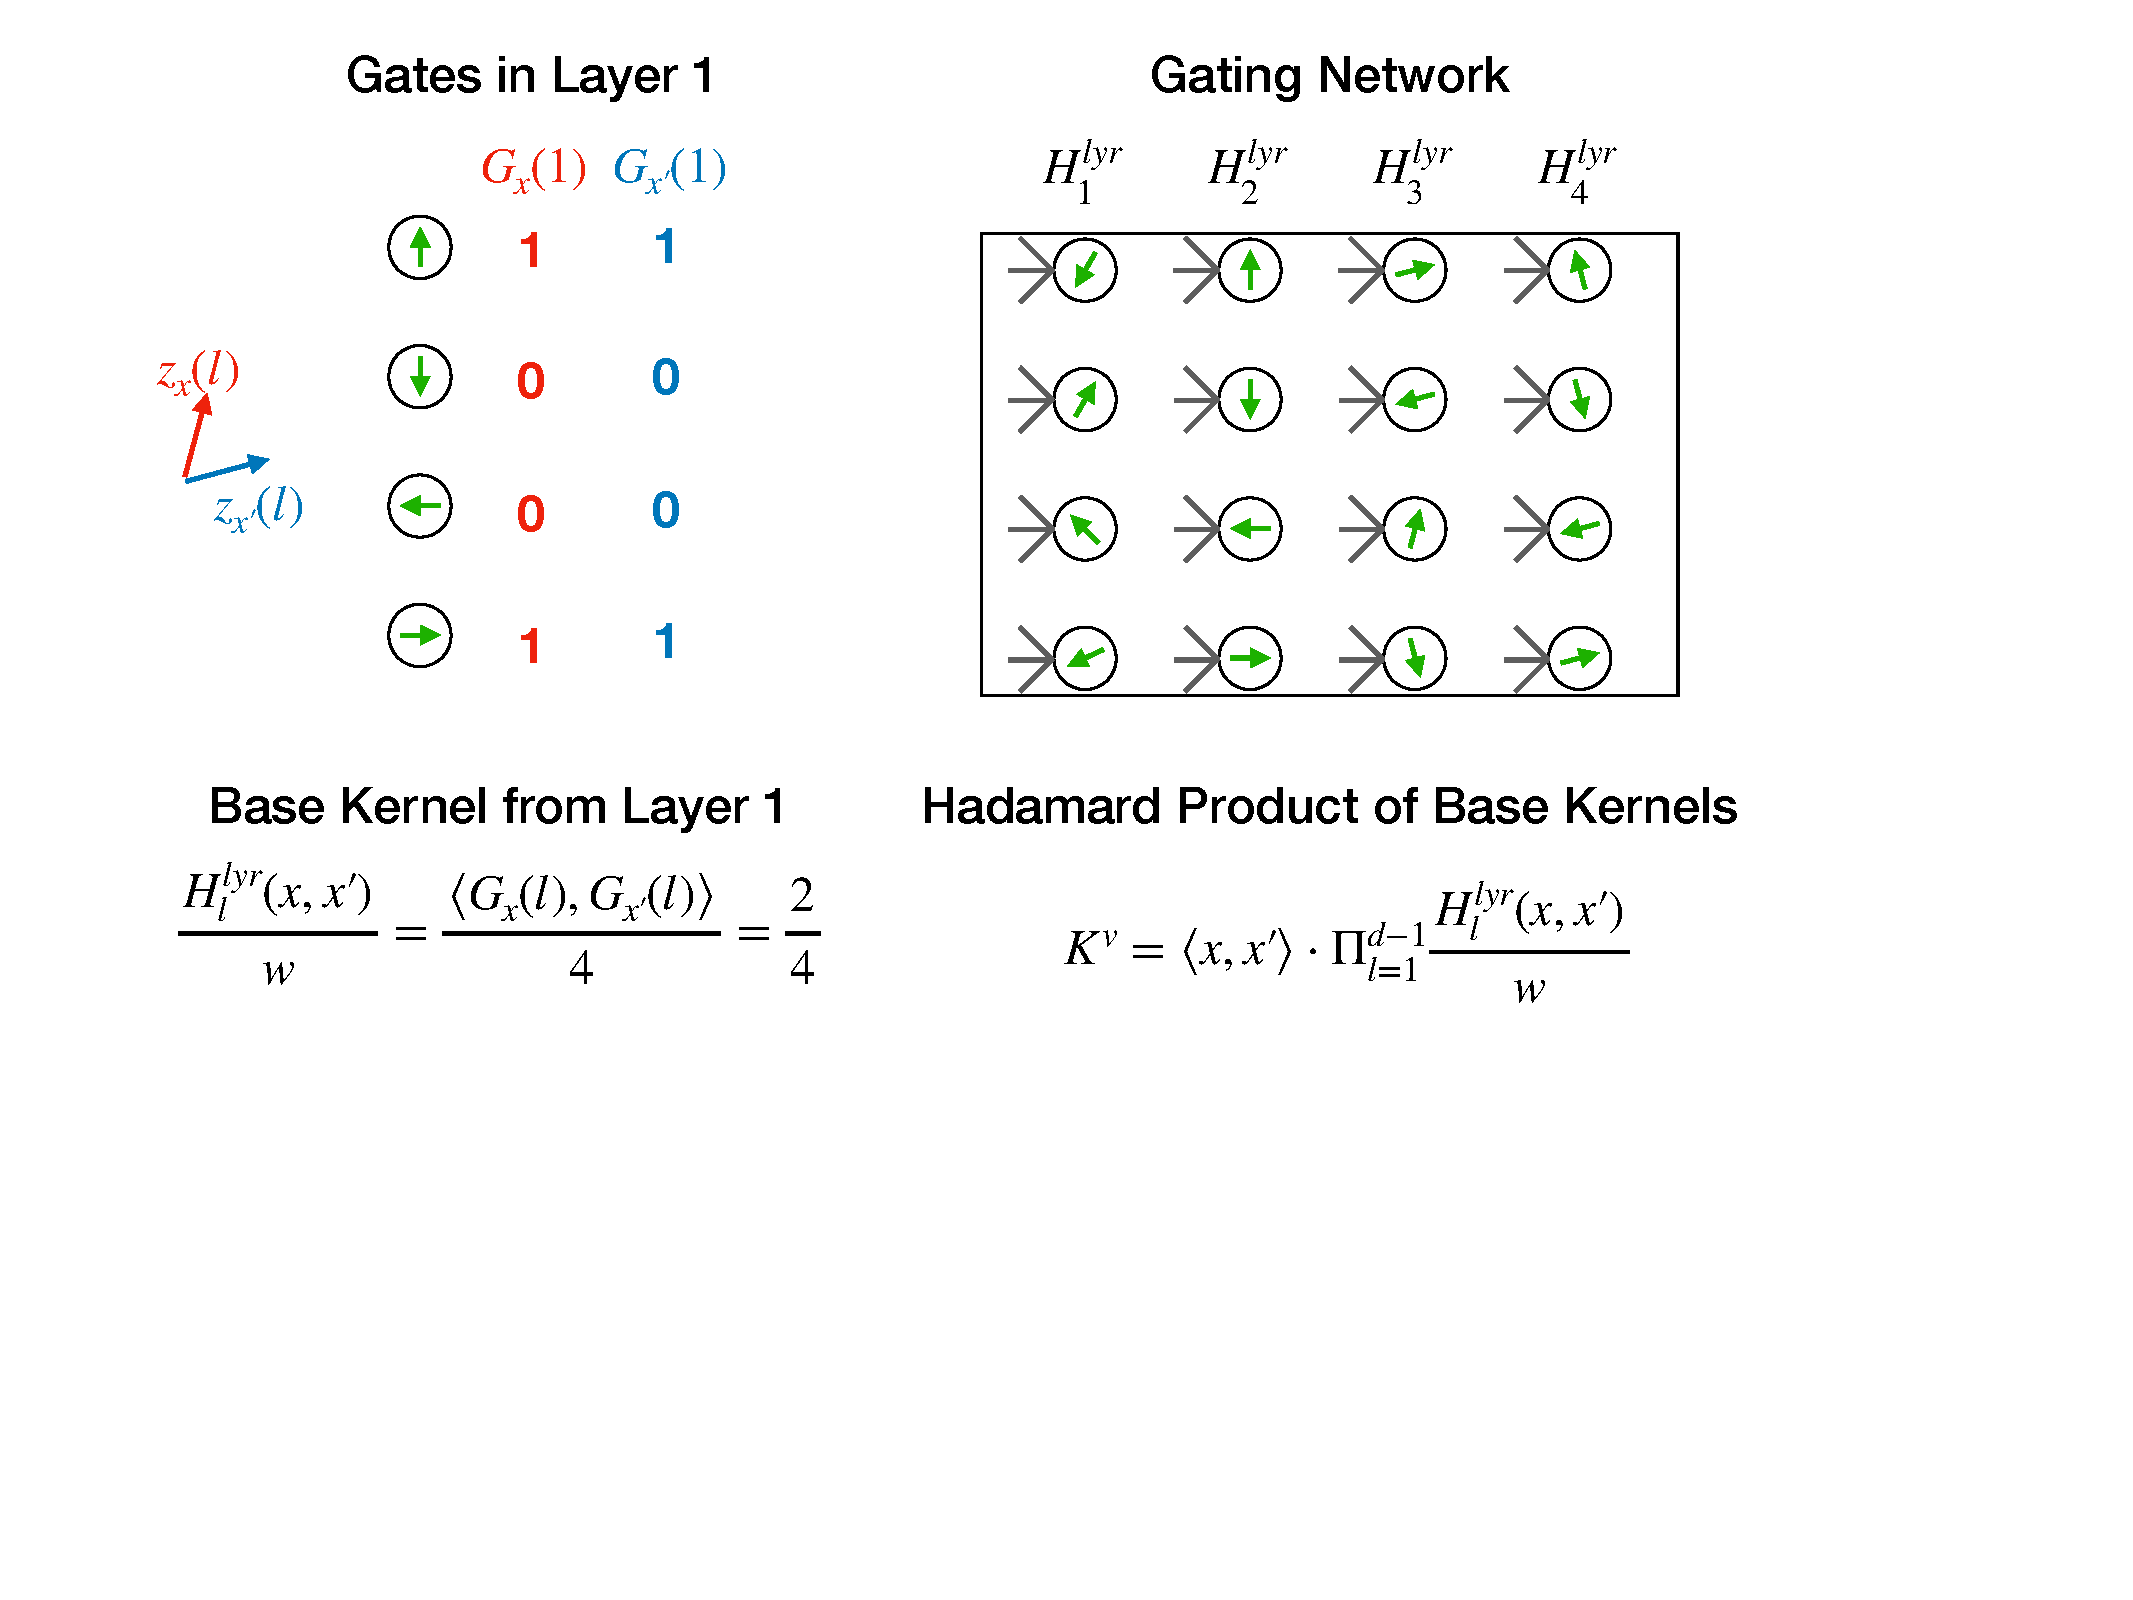
\includegraphics[scale=0.25]{figs/overall.pdf}
\end{figure}
\end{comment}

\section{Skip Connections: Sum of Product Kernel}\label{sec:res}
In this section, we show that in the presence of skip connections, NPK has a sum of product structure. To illustrate our case, we consider a ResNet with `$(b+2)$' blocks and `$b$' skip connections between the blocks (\Cref{fig:resnet}). Each block is a FC-DNN of depth `$\dblock$' and width `$w$'. The sum of product structure is due to the combinatorially many sub-FC-DNNs within this ResNet (see \Cref{def:subfcdnn} and \Cref{fig:subfcdnn}).
\FloatBarrier
\begin{figure}[h]
\resizebox{\columnwidth}{!}{
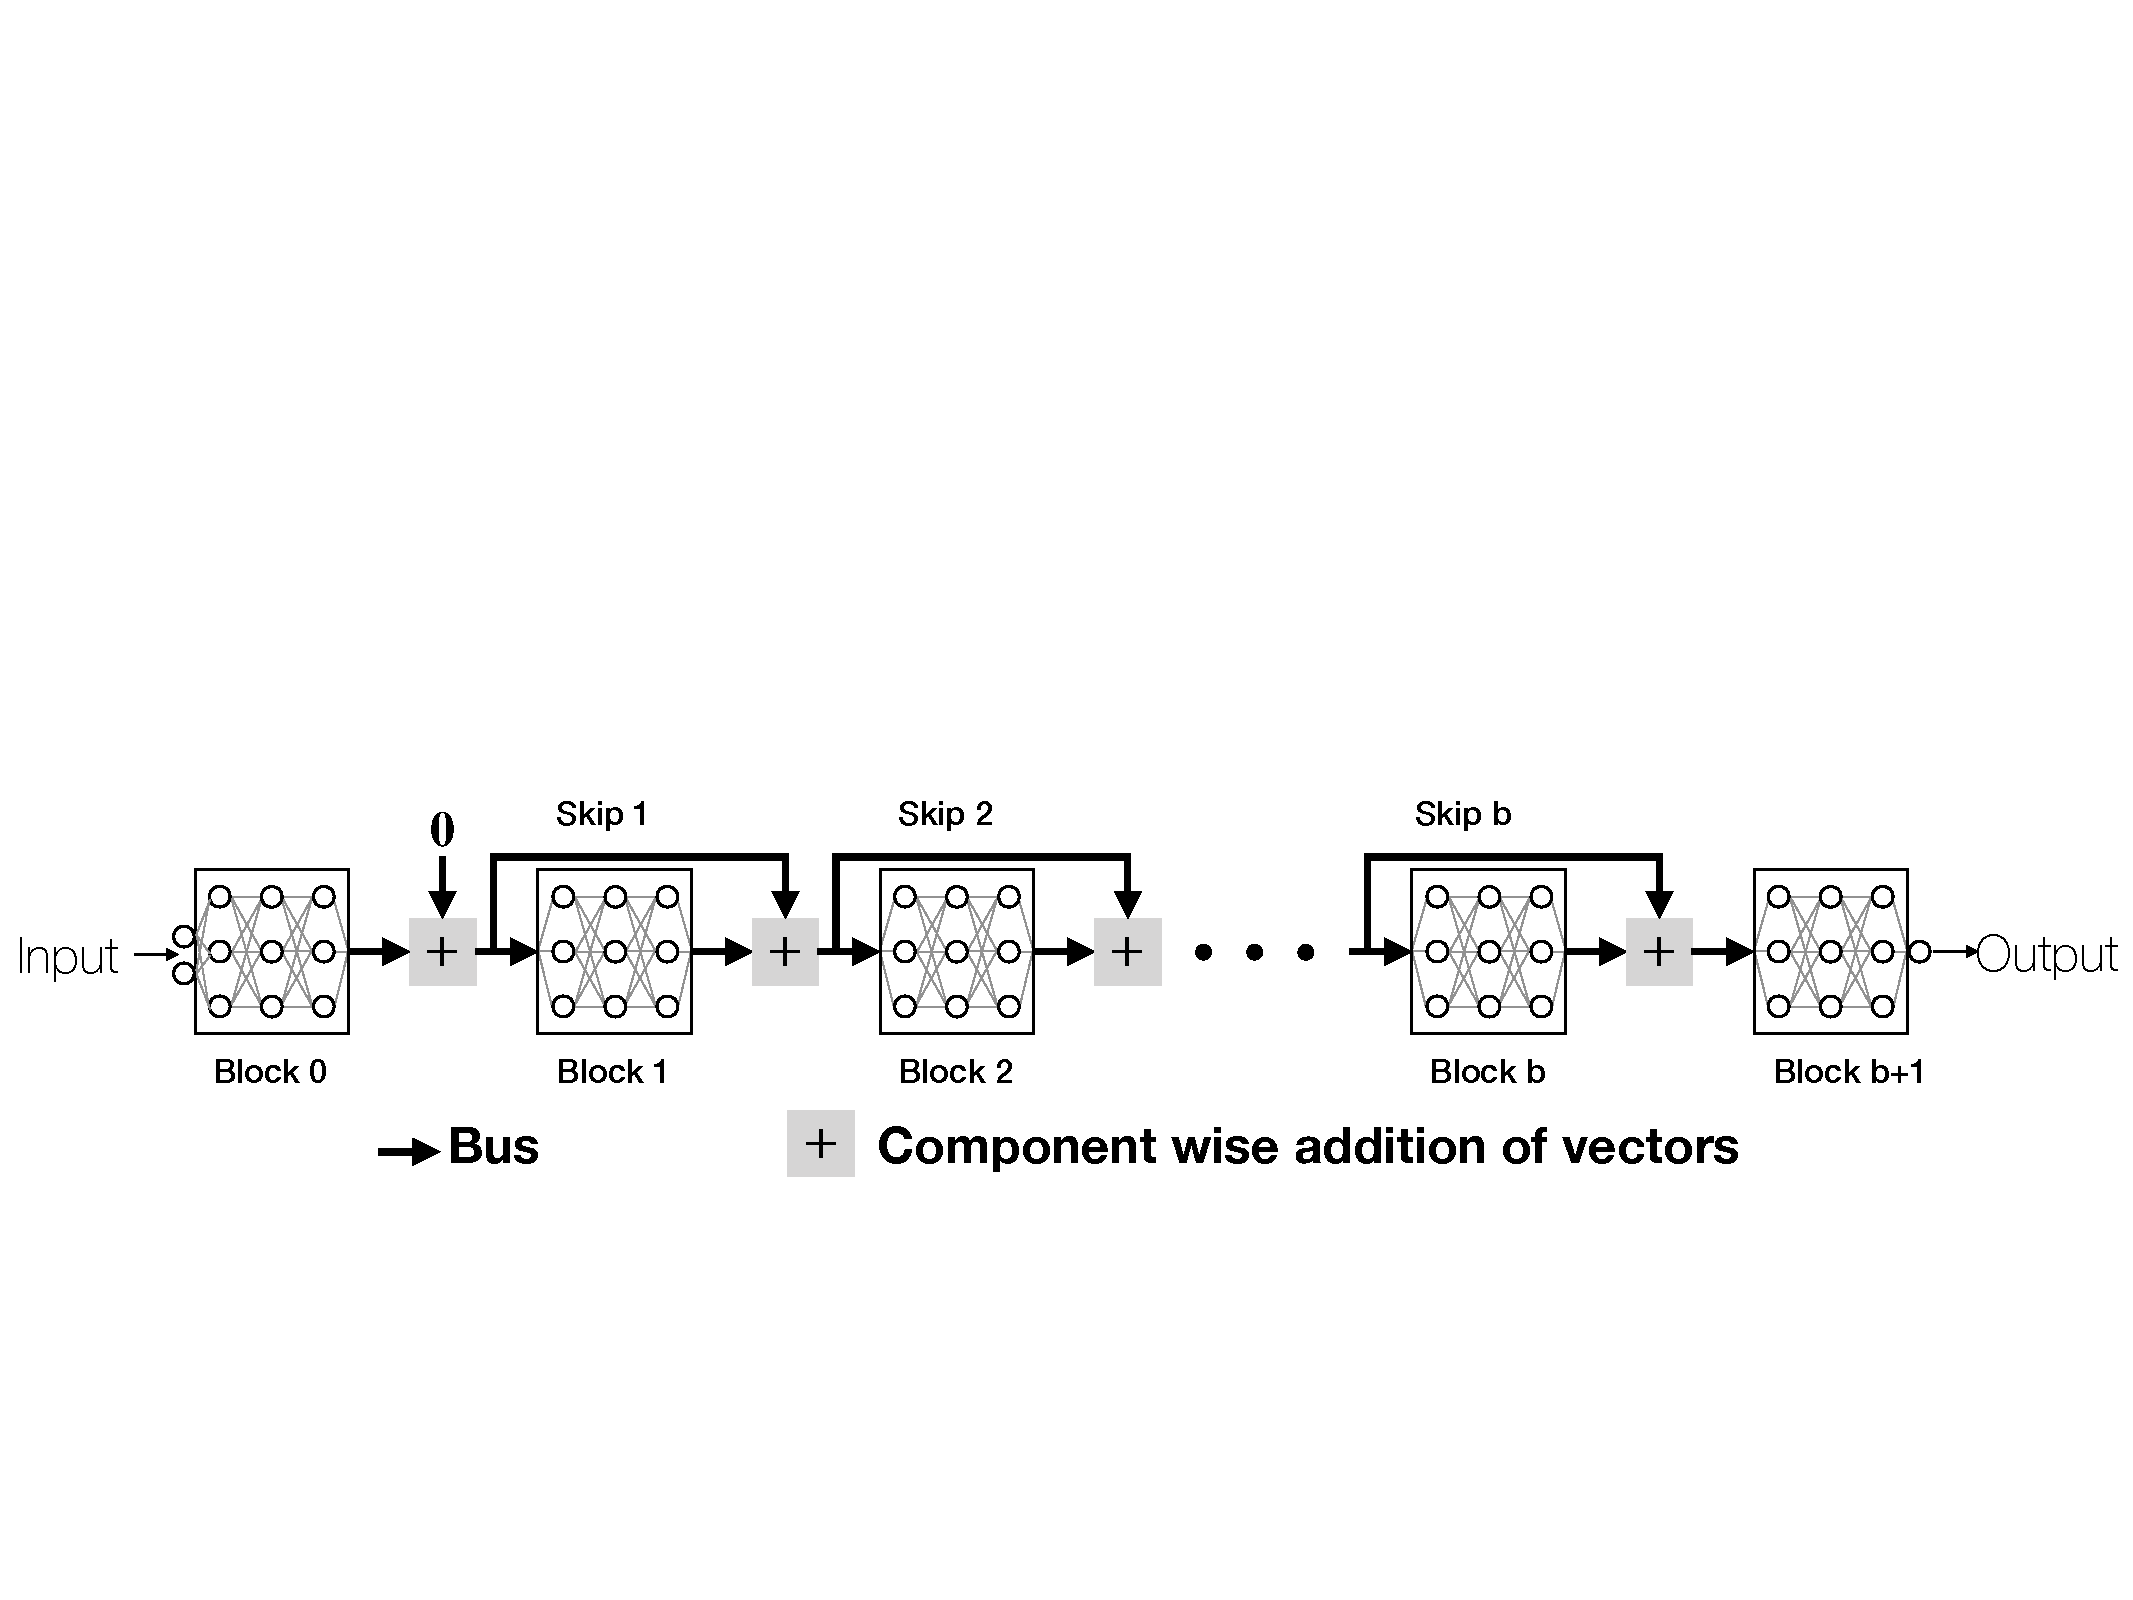
\includegraphics[scale=0.5]{figs/resnet.pdf}
}
\caption{\small{ResNet with $b$ skip connections and $(b+2)$ blocks.}}
\label{fig:resnet}
\end{figure}
\begin{definition}\label{def:subfcdnn}[Sub FC-DNNs]
Let $2^{[b]}$ denote the power set of $[b]$ and let $\J\in 2^{[b]}$ denote any subset of $[b]$. Define the`$\J^{th}$' sub-FC-DNN of the ResNet to be the fully connected network obtained by (i) ignoring/removing (see \Cref{fig:resnet}) the skip connections $\text{skip}_j,\forall j\in \J$  and (ii) ignoring $\text{block}_{j},\forall j\notin \J$ (see \Cref{fig:resnet,fig:subfcdnn}).
\end{definition}
%\Cref{fig:subfcdnn} shows the $4$ sub-FC-DNNs namely $H^i,i=1,2,3,4$ in the case of $b=2$ skip connections.
\FloatBarrier
\begin{figure}[h]
\resizebox{\columnwidth}{!}{
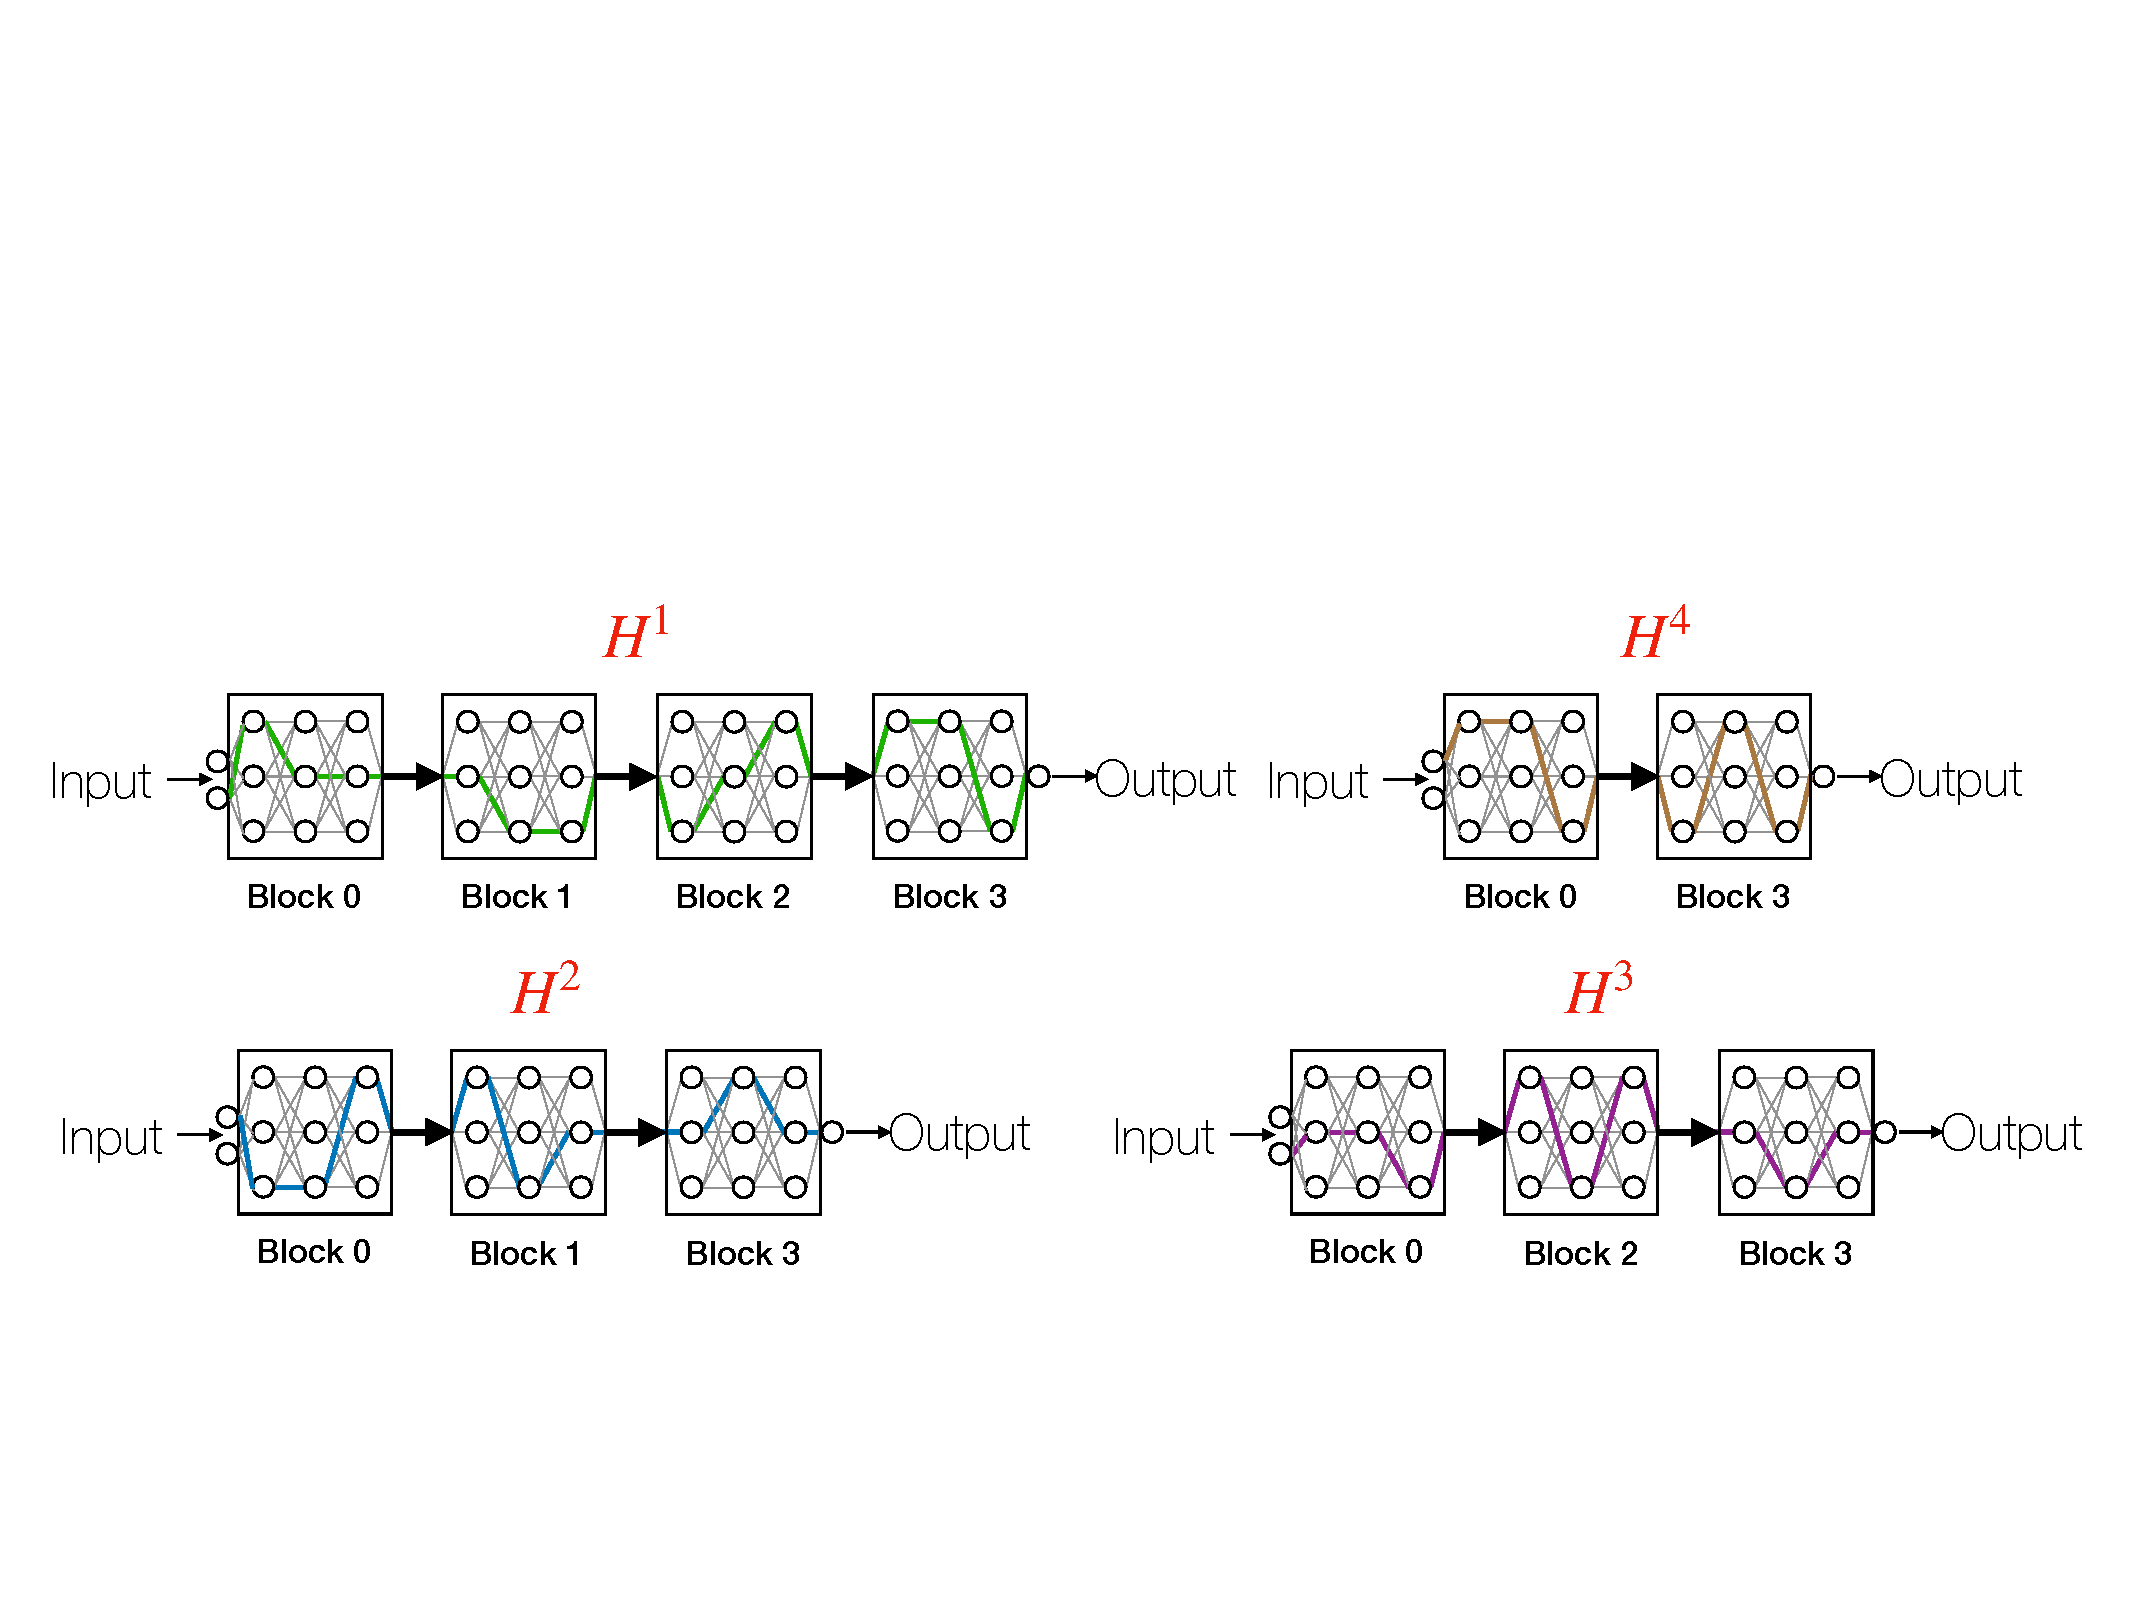
\includegraphics[scale=0.5]{figs/blocks.pdf}
}
\caption{\small{$H^i,i\in[4]$ are the $2^2$ sub-FC-DNNs in a ResNet with $b=2$. Thicker lines in $H^i,i\in[4]$ denote paths. Different grey levels indicate that for $i\neq j$ paths of $H^i$ and $H^j$ are distinct.}}
\label{fig:subfcdnn}
\end{figure}
\begin{comment}
\begin{notation}[Index Maps]
Let $\I^{\J}(p)\colon [\Pres]\ra 2^{[b]}$ specify the indices of the skip connections ignored in path $p$.  Also, we follow the convention that weights and gating values of layers corresponding to blocks skipped are $1$.
\end{notation}
\end{comment}
\begin{lemma}[Sum of Product Kernel]\label{lm:sumofproduct}
Let $H^{\text{res}}_{\Theta}$ be the NPK of the ResNet, and $H^{\J}_{\Theta}$ be the NPK of the sub-FC-DNN within the ResNet obtained by ignoring those skip connections in the set $\J$. Then, \begin{align*}H^{\text{res}}_{\Theta}=\sum_{\J\in 2^{[b]}}H^{\J}_{\Theta}\end{align*}
%\begin{align*}
%\end{align*}
\end{lemma}

\begin{theorem}\label{th:mainres} Let $\sigma=\frac{\cscale}{\sqrt{w}}$. Under \Cref{assmp:main}, as $w\ra\infty$,  for $\bres^{\J} = (|\J| +2)\cdot\dblock\cdot \sigfc^{2\big( (|\J|+2)\dblock-1\big)}$,
\begin{align*}
\kv_{\Tdgn_0}\ra \sum_{\J\in 2^{[b]}}  \bres^{\J} H^{\J}_{\Tf_0}
\end{align*}
\end{theorem}

\section{Role of Convolution with Pooling}

%\section{Architectures: Fully Connected, Convolutional and Residual}\label{sec:arch}
In this section, we present the three architectures that we take up for theoretical analysis. These are i) fully connected (FC or FC-DNN), ii) convolutional (CNN) and iii) residual (ResNets). In what follows, $[n]$ is the set $\{1,\ldots,n\}$, and the dataset is given by $(x_s,y_s)_{s=1}^n\in\R^{\din}\times \R$.

\textbf{Fully Connected:} We consider fully connected networks with width `$w$' and depth `$d$'.
 \FloatBarrier
\begin{table}[h]
\centering
\begin{tabular}{|c l lll|}\hline
Input Layer&: &$z_{x,\Theta}(\cdot,0)$ &$=$ &$x$ \\
Pre-activation&: & $q_{x,\Theta}(\iout,l)$& $=$ & $\sum_{\iin}\Theta(\iin,\iout,l) \cdot z_{x,\Theta}(\iin,l-1) $\\
Gating Value&: &$G_{x,\Theta}(\iout,l)$& $=$ & $\mathbf{1}_{\{q_{x,\Theta}(\iout,l)>0\}}$\\
Hidden Unit Output&: &$z_{x,\Theta}(\iout,l)$ & $=$ & $q_{x,\Theta}(\iout,l)\cdot G_{x,\Theta}(\iout,l)$\\
Final Output&: & $\hat{y}_{\Theta}(x)$ & $=$ & $\sum_{\iin}\Theta(\iin,\iout, d)\cdot z_{x,\Theta}(\iin,d-1)$\\\hline
\end{tabular}
\caption{\small{Information flow in a FC-DNN with ReLU. Here, `$q$'s are pre-activation inputs, `$z$'s are output of the hidden layers, `$G$'s are the gating values. $l\in[d-1]$ is the index of the layer, $\iout$ and $\iin$ are indices of  nodes in the current and previous layer respectively.}}
\label{tb:basic}
\end{table}

\textbf{CNN:} We consider a $1$-dimensional convolutional neural network with circular convolutions (see \Cref{tb:cconv}), with $\dc$ convolutional layers ($l=1,\ldots,\dc$), followed by a \emph{global-average/max-pooling} layer ($l=\dc+1$) and $\dfc$ ($l=\dc+2,\ldots,\dc+\dfc+1$) FC  layers. The convolutional window size is $\wconv<\din$, the number of filters per convolutional layer is $w$, and the width of the FC is also $w$. 
\begin{definition}[Circular Convolution]
For $x\in\R^{\din}$, $i\in[\din]$ and $r\in\{0,\ldots,\din-1\}$, define :

(i) $i\oplus r = i+r$, for $i+r \leq \din$ and $i\oplus r =i+r-\din$, for $i+r>\din$.

(ii) $rot(x,r)(i)=x(i\oplus r), i\in[\din]$.

(iii) $q_{x,\Theta}(\ifout,\iout,l)=\sum_{\icin,\iin}\Theta(\icin,\iin,\iout,l)\cdot z_{x,\Theta}(\ifout\oplus (\icin-1),\iin,l-1)$, where $\iin/\iout$ are the indices (taking values in $[w]$) of the input/output filters. $\icin$ denotes the indices of the convolutional window (taking values in $[\wconv]$) between input and output filters $\iin$ and $\iout$. $\ifout$ denotes the indices (taking values in $[\din]$, the dimension of input features) of individual nodes in a given output filter.
\end{definition}
\begin{definition}[Pooling]
Let $G^{\text{pool}}_{x,\Theta}(\ifout,\iout,\dc+1)$ denote the pooling mask, then we have
\begin{align*}
z_{x,\Theta}(\iout, \dc+1) =\sum_{\ifout} z_{x,\Theta}(\ifout,\iout,\dc)\cdot G^{\text{pool}}_{x,\Theta}(\ifout,\iout,\dc+1),
\end{align*}
where in the case of \emph{global-average-pooling} $G^{\text{pool}}_{x,\Theta}(\ifout,\iout,\dc+1)=\frac{1}{\din},\forall \iout\in[w], \ifout\in[\din]$, and in the case of \emph{$\max$-pooling},  
for a given $\iout\in[w]$, $G^{\text{pool}}_{x,\Theta}(i_{\max},\iout,\dc+1)=1$ where $i_{\max}=\arg\max_{\ifout}z_{x,\Theta}(\ifout,\iout,\dc)$, and $G^{\text{pool}}_{x,\Theta}(\ifout,\iout,\dc+1)=0,\forall \ifout\neq i_{\max}$.
\end{definition}

\textbf{ResNet:} We consider ResNets with `$(b+2)$' blocks and `$b$' skip connections between the blocks (\Cref{fig:resnet}). Each block is a FC-DNN of depth `$\dblock$' and width `$w$'. Here, $\gamma^{\text{pre}}_i,\gamma^{\text{post}}_i,i\in[b]$ are normalisation variables. 
\begin{figure}
\centering
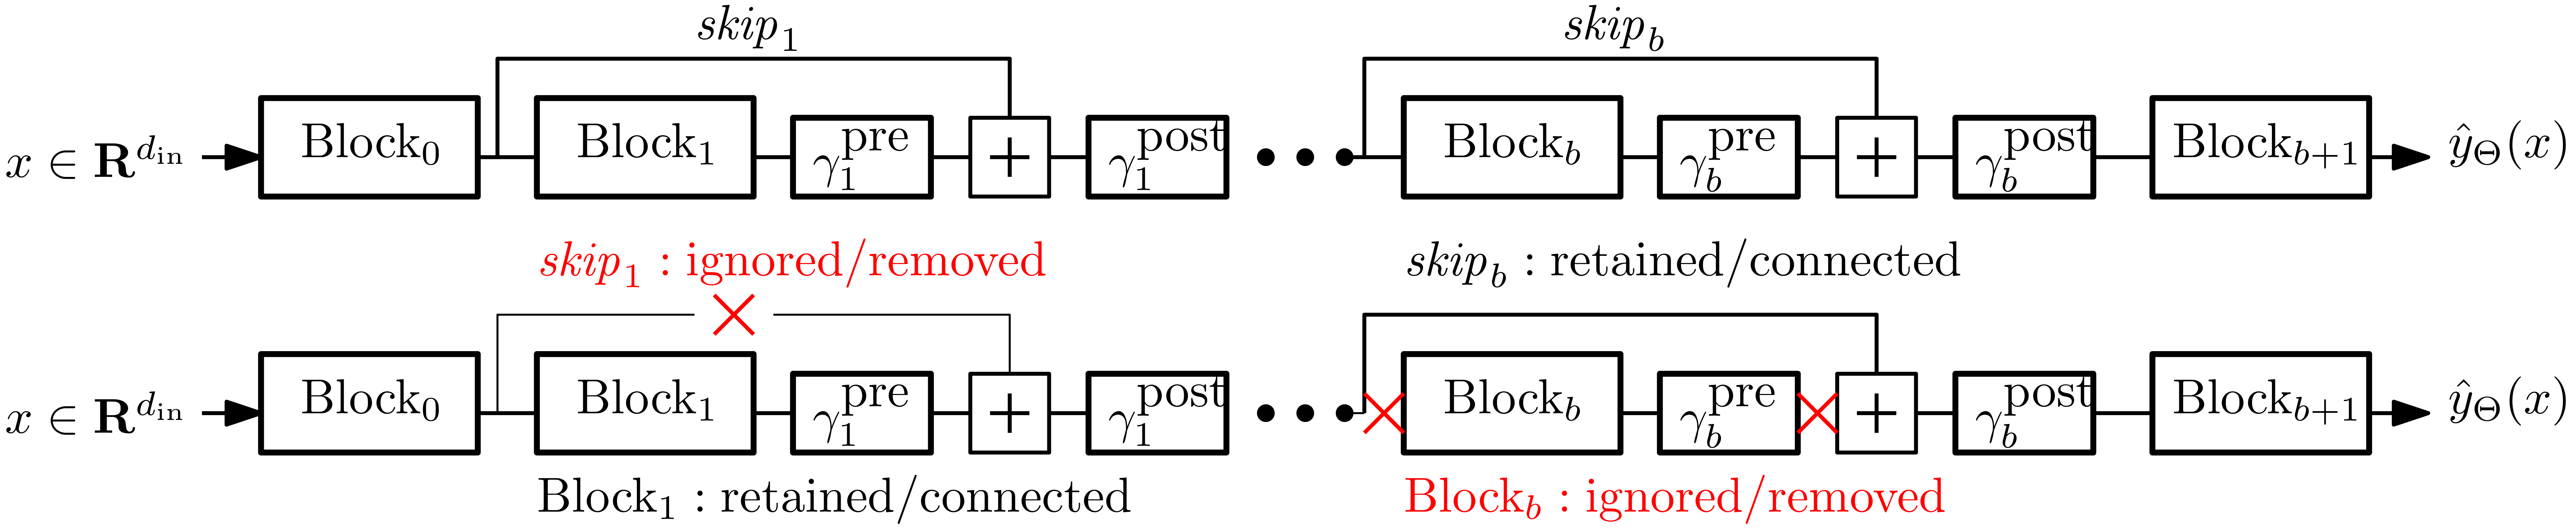
\includegraphics[scale=0.04]{figs/resnet-full.png}
\caption{\small{ResNet Architecture is shown in the top. Process of obtaining a sub-FC-DNN by ignoring skip (retaining block) or retaining skip (ignoring block) is shown in the bottom.}}
\label{fig:resnet}
\end{figure}
\begin{definition}[Sub FC-DNNs]
Let $2^{[b]}$ denote the power set of $[b]$ and let $\J\in 2^{[b]}$ denote any subset of $[b]$. Define the`$\J^{th}$' sub-FC-DNN of the ResNet to be the fully connected network obtained by ignoring/removing (see \Cref{fig:resnet}) the skip connections $\text{skip}_j,\forall j\in \J$ (see \Cref{fig:resnet}).
\end{definition}
\begin{comment}
\FloatBarrier
\begin{figure}[h]
\resizebox{\columnwidth}{!}{
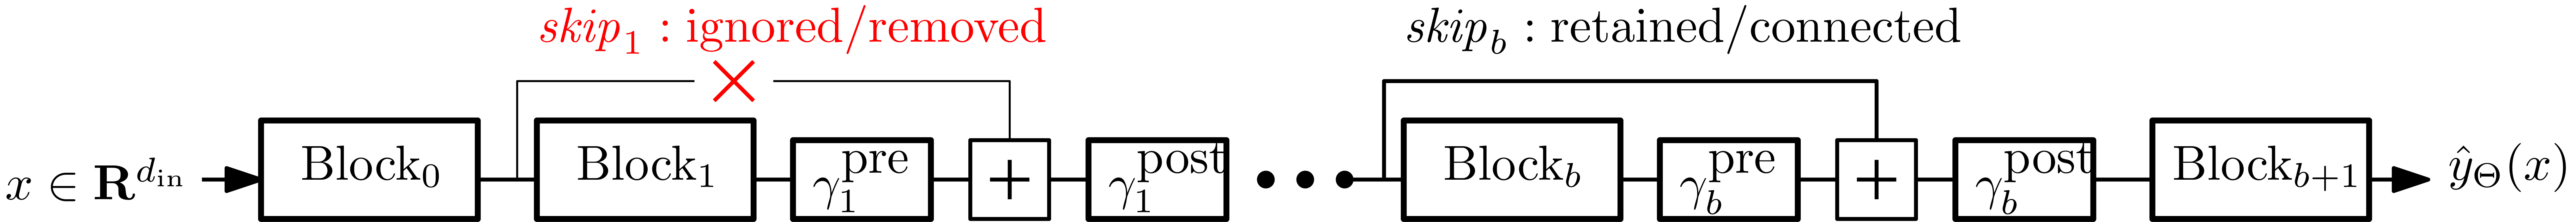
\includegraphics{figs/resnet-ignore.png}
}
\caption{Sub-FC-DNNs within a ResNet.}
\label{fig:resnet-ignore}
\end{figure}
\end{comment}


%\section{Neural Path Framework}\label{sec:npf}
In this section, we extend the \emph{neural path} framework developed by \citetalias{ch2020neural}, to CNN and ResNet architectures described in the previous section. The neural path framework exploits the gating property of ReLU activation, which can be thought of as gate/mask that blocks/allows its pre-activation input depending on its $0/1$ state ( $0$ if pre-activation is negative and $1$ if pre-activation is positive). The key idea here is to  break a DNN (with ReLU) into paths, and express its output as a summation of the contribution of the paths. The contribution of a path is the product of the signal in its input node, the weights in the path and the gates in the path. For a DNN with $P$ paths, for an input $x\in\R^{\din}$,  the gating information is encoded in a novel \emph{neural path feature} (NPF), $\phi_{x,\Theta}\in\R^P$ and a novel \emph{neural path value} (NPV), $v_{\Theta}\in\R^P$ encodes the weights.  The output of the DNN is then the inner product of the NPFs and NPVs, i.e., $\hat{y}_{\Theta}(x_s)=\ip{\phi_{x_s,\Theta},v_{\Theta}}$ (\Cref{prop:zero}).
\begin{definition}
A path starts from an input node, passes through weights, hidden nodes, and normalisation constants and ends at the output node.
\end{definition}
\begin{proposition}
The total number of paths in FC-DNN, CNN and ResNet are respectively given by $\Pfc=\din w^{(d-1)}$,  $\Pcnn=\din(\wconv w)^{\dc}w^{(\dfc-1)}$ and $\Pres = \din \cdot\sum_{i=0}^b \binom{b}{i} w^{(i+2)\dblock-1}$.
\end{proposition}
\begin{notation}[Index Maps]
The ranges of index maps $\Ifeat_l$,  $\Iconv_l$, $\I_l$ are $[\din]$, $[\wconv]$ and $[w]$ respectively. The index maps are used to identify the nodes through which a path $p$ passes. Further, let $\I^{\J}(p)\colon [\Pres]\ra 2^{[b]}$ specify the indices of the skip connections ignored in path $p$.  Also, we follow the convention that weights and gating values of layers corresponding to blocks skipped are $1$.
\end{notation}

\begin{definition}[Path Activity]
The product of the gating values in a path $p$ is its `activity' denoted by $A_{\Theta}(x,p)$. We define:

(a) $A_{\Theta}(x,p)=\Pi_{l=1}^{d-1} G_{x,\Theta}(\I_l(p),l)$, for FC-DNN and ResNet.

(b) $A_{\Theta}(x,p)=\Pi_{l=1}^{\dc+1} G_{x,\Theta}(\Ifeat_l(p),\I_l(p),l)\cdot\Pi_{l=\dc+2}^{\dc+\dfc+1} G_{x,\Theta}(\I_l(p),l)$, for CNN.

In CNN, the pooling layer is accounted by letting $G=G^{\text{pool}}$ for $l=\dc+1$.
\begin{comment}
\emph{
\begin{tabular}{ll}
$A_{\Theta}(x,p)=\Pi_{l=1}^{d-1} G_{x,\Theta}(\I_l(p),l)$& for FC and ResNet\\
$A_{\Theta}(x,p)=\Pi_{l=1}^{\dc} G_{x,\Theta}(\Ifeat_l(p),\I_l(p),l)\cdot G^{\text{pool}}_{x\Theta}(\Ifeat_{\dc+1}(p),\I_{dc+1}(p),\dc+1)\cdot\Pi_{l=\dc+2}^{\dc+\dfc+1} G_{x,\Theta}(\I_l(p),l)$ & for CNN.\\
\end{tabular}
}
\end{comment}
\end{definition}
\begin{comment}
\begin{notation}[Index Map in FC-DNN]
Let $\I_0\colon[P]\ra [\din], \I_{l}\colon [P]\ra [w],l=1,\ldots,d-1, \I_d\colon [P]\ra [1]$ provide the index of the hidden unit through which a path $p$ passes in layer $l$. Further, let $\I^{\J}(p)\colon [\Pres]\ra 2^{[b]}$ specify the indices of the skip connections ignored in path $p$.  Also, we follow the convention that weights and gating values of layers corresponding to blocks skipped are $1$.
\end{notation}
\end{comment}
\begin{comment}
\begin{figure}
\begin{minipage}{0.5\columnwidth}
\begin{tabular}{|l|l|}\hline
Index Map & Layers\\\hline
$\Ifeat_{l}\colon [P]\ra[\din]$ & $l=0$\\\hline
$\Iconv_{l}\colon [P]\ra[\wconv]$ & $l=0,\ldots,\dc$\\\hline
$\Iwidth_{l}\colon [P]\ra[1]$  & $l=0$\\ \hline
$\Iwidth_{l}\colon [P]\ra[w]$  & $l=1,\ldots,\dc+\dfc$\\ \hline
$\Iwidth_{l}\colon [P]\ra[1]$  & $l=\dc+\dfc+1$\\ \hline
\end{tabular}
\end{minipage}
\begin{minipage}{0.5\columnwidth}
\resizebox{\columnwidth}{!}{
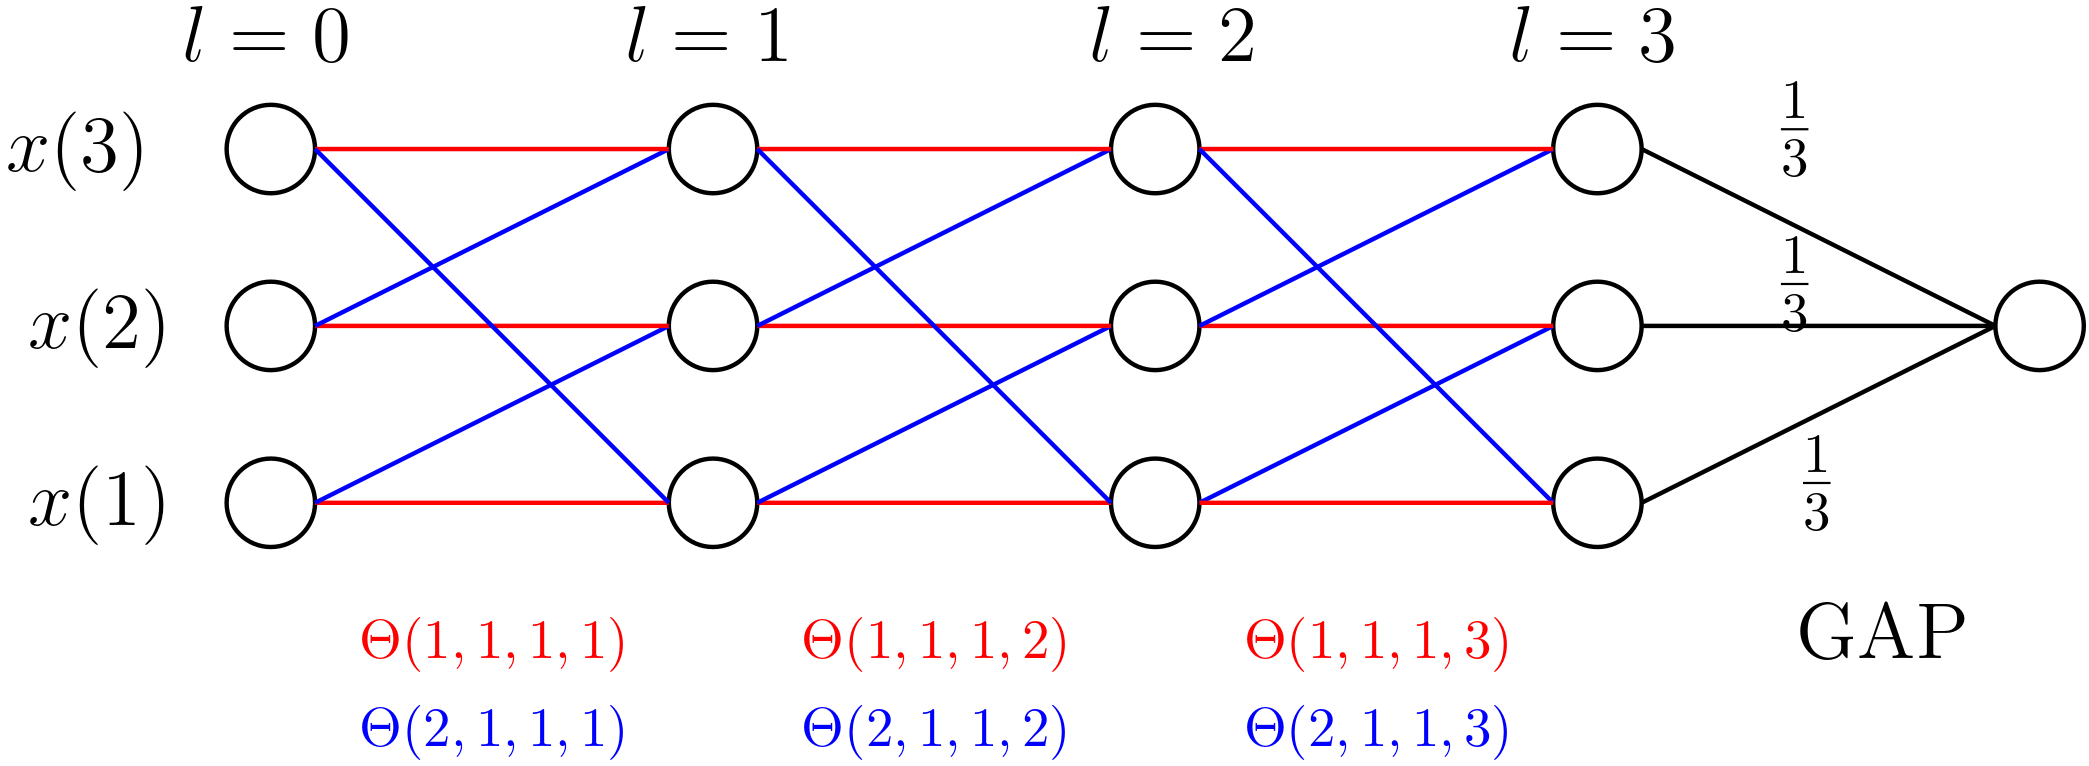
\includegraphics[scale=0.1]{figs/pathshare.png}
}
\end{minipage}
\end{figure}
\end{comment}
\begin{comment}
\begin{notation}[Index Map in ResNet] $\I_0\colon[\Pres]\ra [\din]$, $\I_{l}\colon [\Pres]\ra [w]l=1,\ldots,\dblock, (b+1)\dblock,\ldots,(b+2)\dblock-1$, $\I_{l}\colon [\Pres]\ra [w]\cup\emptyset, l=\dblock+1,\ldots,(b+1)\dblock$. Further, let $\I^{\J}(p)\colon [\Pres]\ra 2^{[b]}$ specify the indices of the skip connections ignored in path $p$. Also, $\emptyset$ denotes an empty index and we follow the convention that weights and gating values through empty indices are $1$.
\end{notation}
\end{comment}
\begin{comment}
\begin{definition}[Index Map in ResNet]
The index maps that specify the weights through which a given path $p$ passes are specified as given below.
\begin{center}
\begin{tabular}{|c|l|}\hline
Index Set & Layer\\\hline
$\I_l\colon[\Pres]\ra [\din]$ & $l=0$\\\hline
$\I_{l}\colon [\Pres]\ra [w]$ &  $l=1,\ldots,\dblock$ and $l=(b+1)\dblock,\ldots,(b+2)\dblock-1$\\\hline
$\I_{l}\colon [\Pres]\ra [w]\cup\emptyset$ &  $l=\dblock+1,\ldots,(b+1)\dblock$\\\hline
\end{tabular}
\end{center}
Further, let $\I^{\J}(p)\colon [\Pres]\ra 2^{[b]}$ specify the indices of the skip connections ignored in path $p$. Also, $\emptyset$ denotes an empty index and we follow the convention that weights and gating values through empty indices are $1$.
\end{definition}
\end{comment}
\begin{definition}[Bundle Paths of Sharing Weights]\label{def:bundle}
Let $\hat{P}^{\text{cnn}}=\frac{\Pcnn}{\din}$, and $\{B_1,\ldots, B_{\hat{P}^{\text{cnn}}}\}$ be a collection of sets such that $\forall i,j\in [\hat{P}^{\text{cnn}}], i\neq j$ we have $B_i\cap B_j=\emptyset$ and $\cup_{i=1}^{\hat{P}^{\text{cnn}}}B_i =[\Pcnn]$. Further,  if paths $p,p' \in B_i$, then $\Iconv_l(p)=\Iconv_l(p'), \forall l=1,\ldots, \dc$ and $\I_l(p)=\I_l(p'), \forall l=0,\ldots, \dc$.
\end{definition}
\begin{proposition}\label{prop:bundle}
There are exactly $\din$ paths in a bundle.
\end{proposition}

\begin{definition}[Normalisation Factor]
Define $\Gamma(\J)\eqdef \underset{j\in J}\Pi \gamma^{\text{pre}}_j \cdot \underset{j'\in [b]}\Pi \gamma^{\text{post}}_{j'}$
\end{definition}
 Weight sharing is shown in the the cartoon in \Cref{fig:pathshare}, which shows a CNN with $\din=3$, $w=1$, $\wconv=2$, $\dc=3$, $\dfc=0$. Here, the red coloured paths all share the same weights  $\Theta(1,1,1,l), l=1,2,3$ and the blue coloured paths all share the same weights given by $\Theta(2,1,1,l), l=1,2,3$. 
\FloatBarrier
 \begin{figure}[h]
\begin{minipage}{0.33\columnwidth}
\resizebox{\columnwidth}{!}{
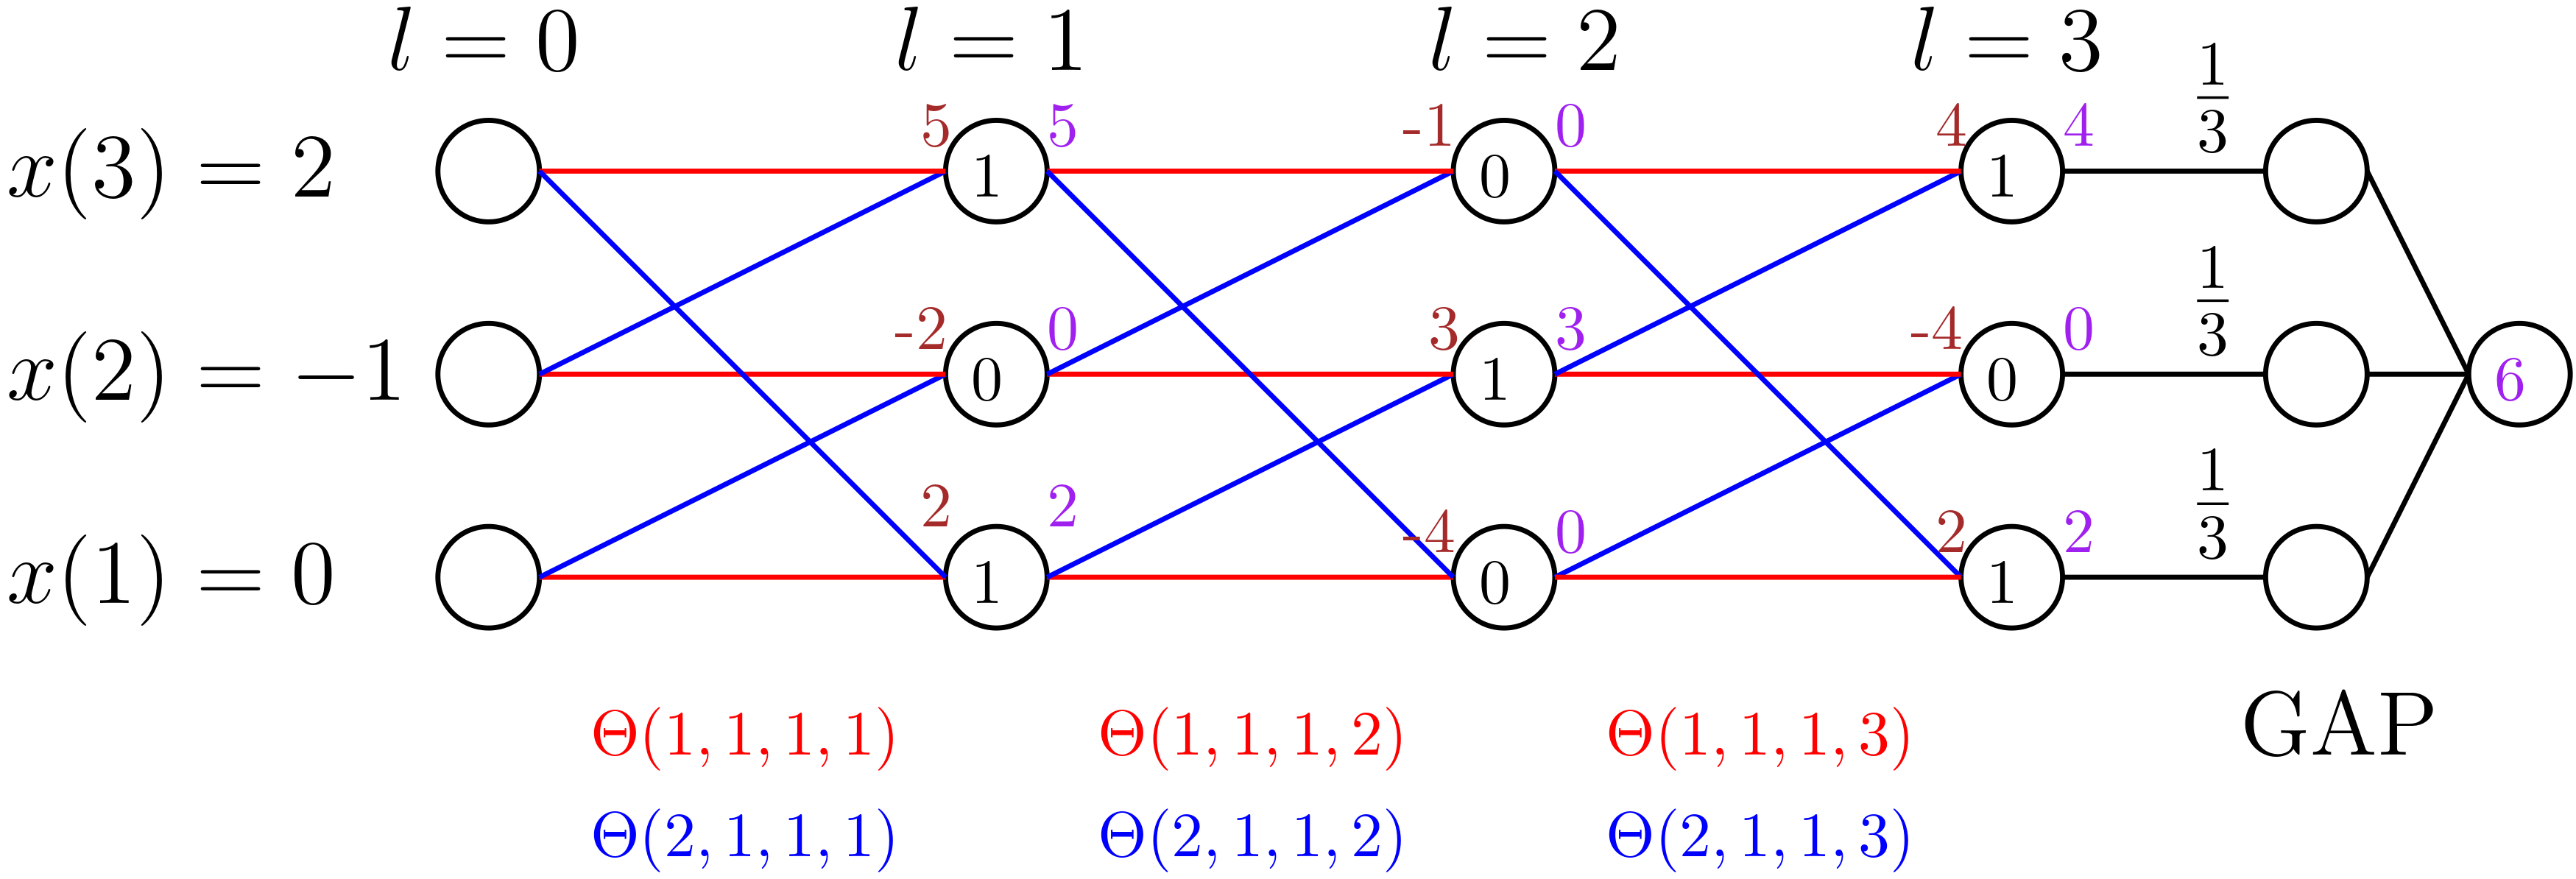
\includegraphics[angle=0.2,scale=0.1]{figs/gap.png}
}
\end{minipage}
\begin{minipage}{0.33\columnwidth}
\resizebox{\columnwidth}{!}{
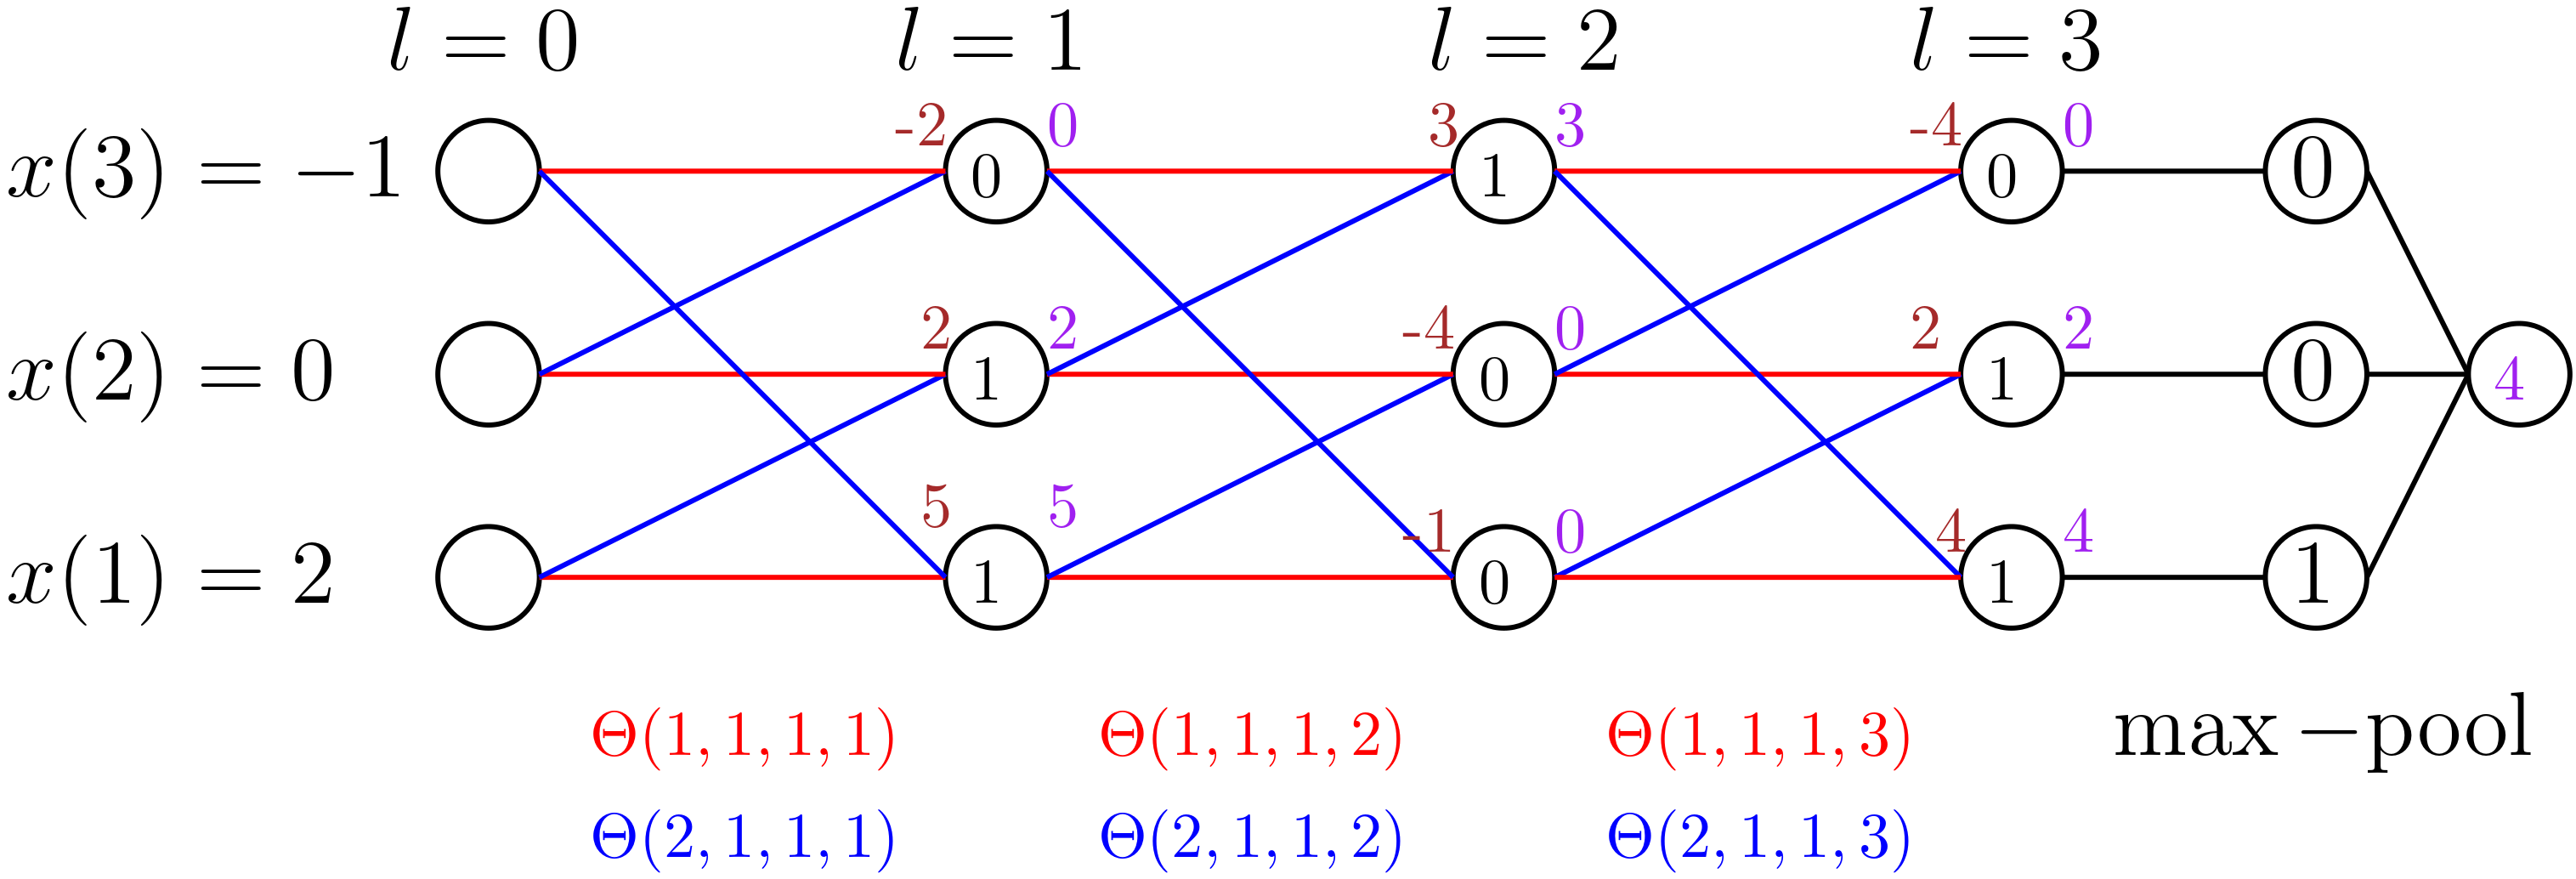
\includegraphics[angle=0.2,scale=0.1]{figs/maxp1.png}
}
\end{minipage}
\begin{minipage}{0.33\columnwidth}
\resizebox{\columnwidth}{!}{
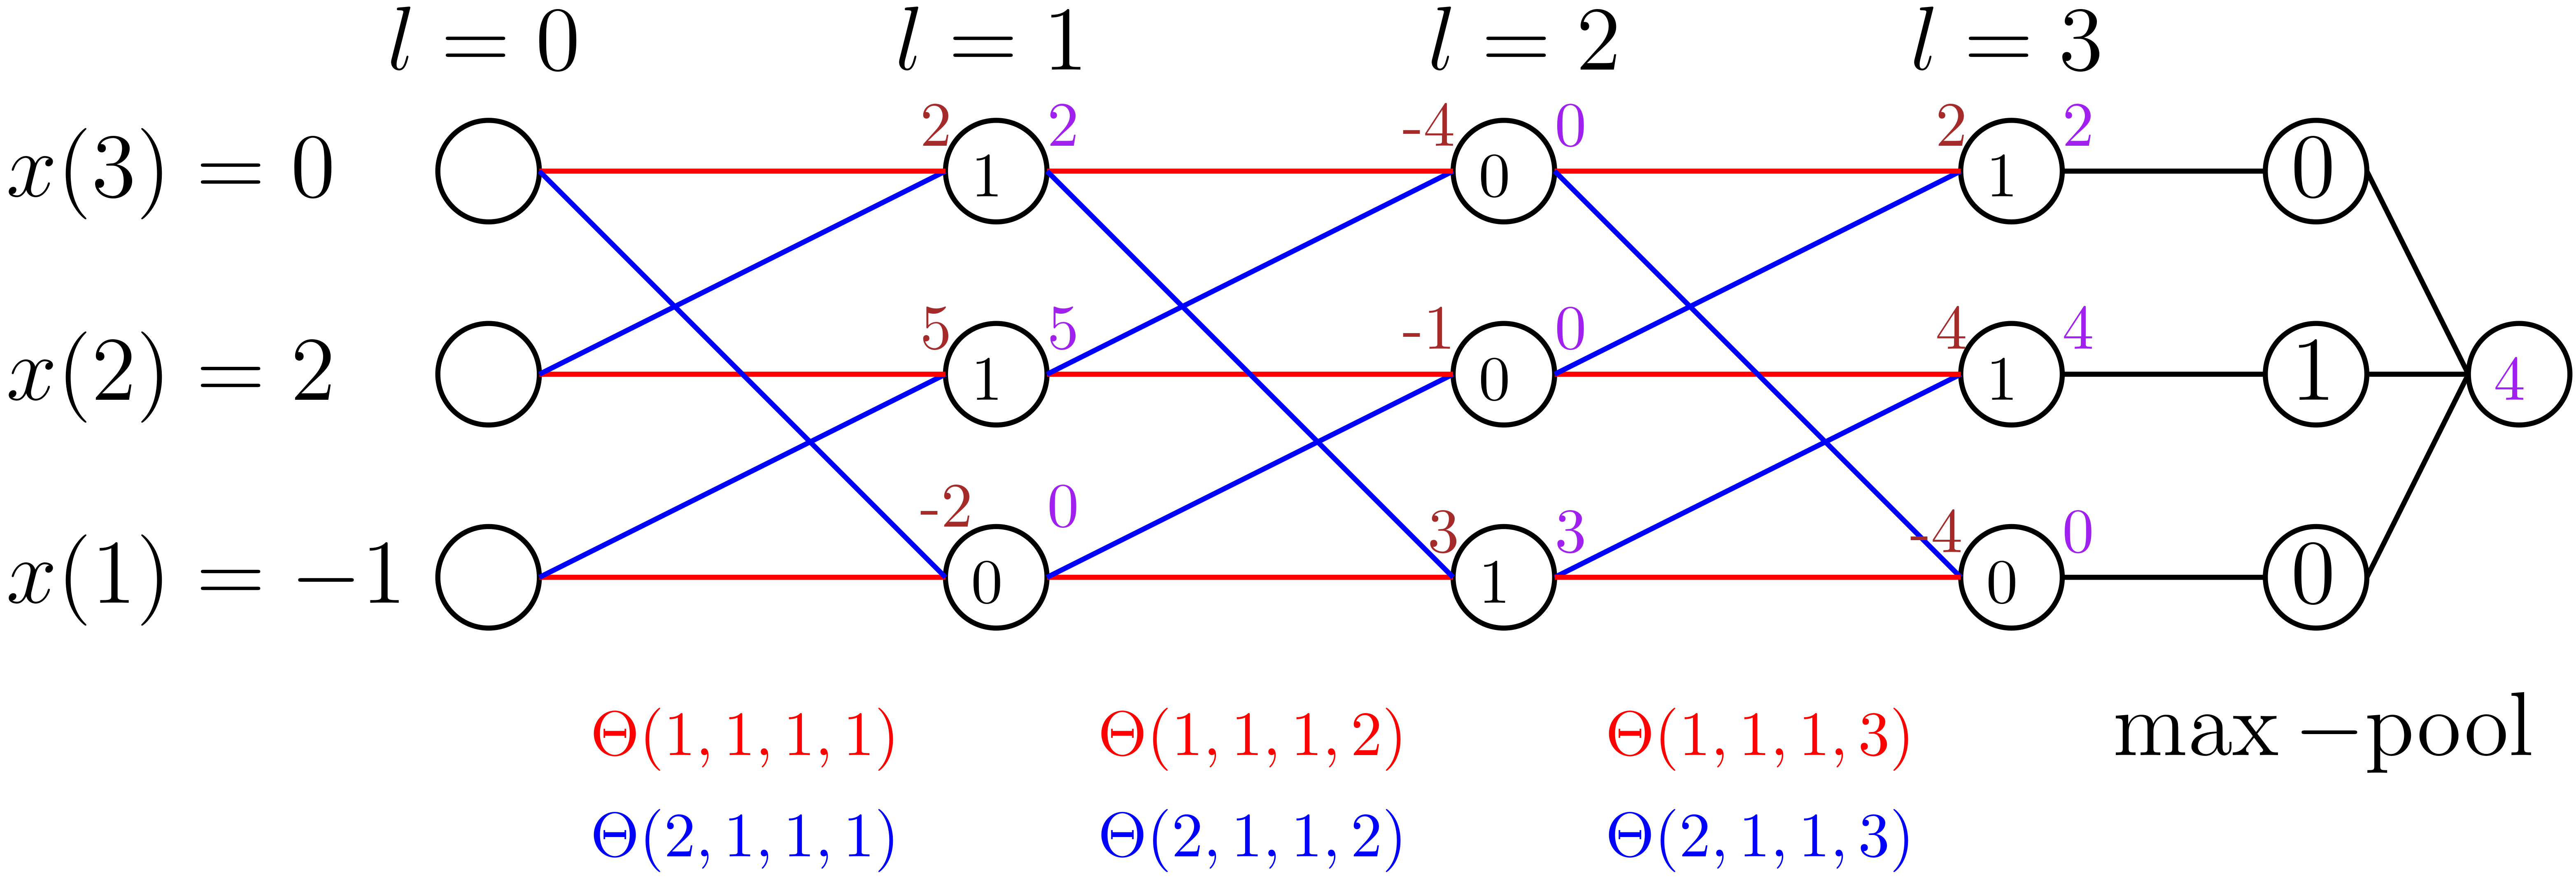
\includegraphics[angle=0.2,scale=0.1]{figs/maxp2.png}
}
\end{minipage}
\caption{\small{Shows weight sharing and rotational symmetry of internal variables and the output after pooling in a CNN. Left most cartoon uses a GAP layer, and the other two cartoons use $\max$-pooling. Circles are nodes and the $1/0$ in the nodes indicate the gating. Pre-activations/node output are shown in {\color{chocolate}{brown}}/{\color{electricpurple}{purple}}.}}
\label{fig:pathshare}
\end{figure}
\begin{definition}[Neural Path Value]
The product of the weights and normalisation factors in a path $p$ is its `value'. The value of a path bundle is the value of any path in that bundle. The path/bundle values are denoted by $v_{\Theta}(p)/v_{\Theta}(B_{\hat{p}})$ and are defined as follows:

(a) $v_{\Theta}(p)=\Pi_{l=1}^d \Theta(\I_{l-1}(p),\I_l(p),l)$.


(b) $v_{\Theta}(B_{\hat{p}})= \Pi_{l=1}^{\dc} \Theta(\Iconv_{l}(p),\I_{l-1}(p),\I_{l}(p),l) \cdot \Pi_{l=\dc+2}^{\dc+\dfc+1} \Theta(\I_{l-1}(p),\I_l(p),l)$, for any $p\in B_{\hat{p}}$.

(c) $v_{\Theta}(p)=\Pi_{l=1}^d \Theta(\I_{l-1}(p),\I_l(p),l) \cdot \Gamma(\I^{\J}(p))$.

The neural path value is defined as $v_{\Theta}\eqdef (v_{\Theta}(p),p\in [\Pfc])\in\R^{\Pfc}$, $v_{\Theta}\eqdef (v_{\Theta}(B_{\hat{p}}),\hat{p}\in [\hat{P}^{\text{cnn}}])\in\R^{\hat{P}^{\text{cnn}}}$, and $v_{\Theta}\eqdef (v_{\Theta}(p),p\in [\Pres])\in\R^{\Pres}$ for FC-DNN, CNN and ResNet respectively.
 \end{definition}
\begin{proposition}[Rotational Invariance]\label{prop:rot}
Internal variables in the convolutional layers are circularly symmetric,  i.e., for $r\in\{0,\ldots,\din-1\}$ it follows that (i) $z_{rot(x,r),\Theta}(\ifout,\cdot,\cdot) = z_{x,\Theta}(\ifout \oplus r,\cdot,\cdot)$, (ii) $q_{rot(x,r),\Theta}(\ifout,\cdot,\cdot) = q_{x,\Theta}(\ifout \oplus r,\cdot,\cdot)$ and (iii) $G_{rot(x,r),\Theta}(\ifout,\cdot,\cdot) = G_{x,\Theta}(\ifout \oplus r,\cdot,\cdot)$.
\end{proposition}
\begin{definition}
The neural path feature (NPF) corresponding to a path $p$ is given by 

(a) $\phi_{x,\Theta}(p)\eqdef  x(\Ifeat_0(p))A_{\Theta}(x_s,p)$ for  FC-DNN and ResNet.

(b) $\phi_{x,\Theta}(\hat{p})\eqdef \sum_{\hat{p}\in B_{\hat{p}}}x(\Ifeat_0(p))A_{\Theta}(x,p)$ for CNN.

The NPF is defined as $\phi_{x,\Theta}\eqdef (\phi_{x,\Theta}(p),p\in [\Pfc])\in\R^{\Pfc}$, $\phi_{x,\Theta}\eqdef (\phi_{x,\Theta}(B_{\hat{p}}),\hat{p}\in [\hat{P}^{\text{cnn}}])\in\R^{\hat{P}^{\text{cnn}}}$, and $\phi_{x,\Theta}\eqdef (\phi_{x,\Theta}(p),p\in [\Pres])\in\R^{\Pres}$ for FC-DNN, CNN and ResNet respectively.
\end{definition}
\begin{proposition}[Output=$\langle$NPF,NPV$\rangle$]\label{prop:zero}  The output of the network can be written as an inner product of the NPF and NPV, i.e., 
$\hat{y}_{\Theta}(x)=\ip{\phi_{x,\Theta},v_{\Theta}}$.
\end{proposition}
\begin{comment}
\FloatBarrier
\begin{table}[h]
\resizebox{\columnwidth}{!}{
\begin{tabular}{|c|c|c|c|}\hline
Quantity& FC& CNN & ResNet\\\hline
%Total Paths & $\Pfc=\din w^{(d-1)}$ & $\Pcnn=\din(\wconv w)^{\dc}w^{(\dfc-1)}$ & $\Pres = \din \cdot\sum_{i=0}^b \binom{b}{i} w^{(i+2)\dblock-1}$\\\hline
%Path-per Bundle& $1$ & $\din$ &$1$\\\hline
$A_{\Theta}(x,p)$	&$\Pi_{l=1}^{d-1} G_{x,\Theta}(\I_l(p),l)$ &\shortstack{$\left(\Pi_{l=1}^{\dc} G_{x,\Theta}(\Ifeat_l(p),\Iconv_l(p),l)\right)$ \\ $\cdot \left(\Pi_{l=\dc+2}^{\dc+\dfc+1} G_{x,\Theta}(\Ifc_l(p),l)\right)$} &  $\Pi_{l=1}^{d-1} G_{x,\Theta}(\I_l(p),l)$\\\hline 
$\phi_{x,\Theta}(p)$ & $x(\I_0(p))A_{\Theta}(x_s,p)$ & $\sum_{\hat{p}\in B_{\hat{p}}}x(\Ifeat_0(p))A_{\Theta}(x,p)$ & $x(\I_0(p))A_{\Theta}(x_s,p)$\\\hline

$v_{\Theta}(p)$ & $\Pi_{l=1}^d \Theta(\I_{l-1}(p),\I_l(p),l)$ &$ v_{\Theta}(B_{\hat{p}}$ &\shortstack{$  \Pi_{l=1}^d \Theta(\I_{l-1}(p),\I_l(p),l)\cdot$\\ $\Gamma(\I^{\J}(p))$}\\\hline
\end{tabular}
}
\end{table}
\end{comment}

%\section{Neural Path Kernel: Composite Kernel Based on sub-networks}\label{sec:npk}
In this section, we will discuss the properties of \emph{neural path kernel} (NPK) associated with the NPFs defined in \Cref{sec:npf}. Recall that a co-ordinate of NPF can be non-zero only if the corresponding path is active. Consequently, the NPK for a pair of input examples is a similarity measure that depends on the number of paths that are active for both examples. Such common active paths are captured in a quantity denoted by $\Lambda$ (\Cref{def:cnnlambda}). The number of active paths are in turn dependent on the number of active gates in each layer, a fact that endows the NPK with a hierarchical/composite structure. Gates are the basic building blocks, and the gates in a layer for a $w$-dimensional binary feature whose kernels are the base kernels. When the layers are laid out depth-wise, we obtain a product of the base kernels. When skip connections are added, we obtain a sum of products of base kernels. And presence of convolution with pooling  provides rotational invariance. 

\begin{definition}
Define the NPK matrix to be  $H_{\Theta}\eqdef\Phi^\top_{\Theta}\Phi_{\Theta}$, where $\Phi_{\Theta}=(\phi_{x_1,\Theta},\ldots,\phi_{x_n,\Theta})\in\R^{P\times n}$ is the NPF matrix.
\end{definition}
\begin{comment}
As a result, it turns out that, depending on the network architecture, the NPK has interesting structure/form. In FC-DNN, the NPK involves product of base kernels (\Cref{def:layerkernel},\Cref{lm:productkernel}) corresponding to the binary gating features of the various layers. In ResNet with $b$ skip connections there are $2^b$ sub-FC-DNNs and the NPK is a sum of the NPKs of these sub-FC-DNNs (\Cref{lm:sumofproduct}). Further, in CNNs due to weight sharing, the NPK has a rotationally invariant form (\Cref{lm:cnnnpk}). In what follows, we define the NPK matrix to be  $H_{\Theta}\eqdef\Phi^\top_{\Theta}\Phi_{\Theta}$, where $\Phi_{\Theta}=(\phi_{x_1,\Theta},\ldots,\phi_{x_n,\Theta})\in\R^{P\times n}$ is the NPF matrix.
\end{comment}
\begin{definition}\label{def:cnnlambda}
 Define $\Lambda_{\Theta}(i,x,x_{s'}) \eqdef \left|\{p\in[P]\colon  \I_0(p)=i, A_{\Theta}(x_s,p)= A_{\Theta}(x_{s'},p)=1\}\right|$ to be total number of `active' paths for both $x_s$ and $x_{s'}$ that pass through input node $i$.
\end{definition}
%\subsection{NPK of FC-DNN: Product Kernel }
%\input{cnpkexample}
%\subsection{Neural Path Kernel : Similarity based on active sub-networks}
\begin{definition}[Layer-wise Kernel]\label{def:layerkernel} Let $G_{x,\Theta}(\cdot,l)\in\R^w$ be $w$-dimensional feature of the gating values in layer $l$ for input $x\in\R^{\din}$.  Define layer-wise kernels:
\begin{align*}
H^{\text{lyr}}_{l,\Theta}(s,s')\eqdef\ip{G_{x_s,\Theta}(\cdot,l)G_{x_{s'},\Theta}(\cdot,l)}
\end{align*}
\end{definition}
\begin{lemma}[Product Kernel]\label{lm:productkernel}
 Let $H^{\text{fc}}$ denote the NPK of a FC-DNN, and for $D\in\R^{\din\times\din}$ be a diagonal matrix with strictly positive entries, and $u,u'\in\R^{\din}$ let $\ip{u,u'}_{D}=\sum_{i=1}^{\din}D(i)u(i)u'(i)$.
\begin{align*}
H^{\text{fc}}_{\Theta}(s,s')= \ip{x_s,x_{s'}}_{\Lambda(\cdot,x_s,x_{s'})}=\ip{x_s,x_s'}\Pi_{l=1}^{d-1}H^{\text{lyr}}_{l,\Theta}(s,s')\end{align*}
\end{lemma}
%\subsection{NPK of ResNet: Sum of Product Kernel}
\begin{lemma}[Sum of Product Kernel]\label{lm:sumofproduct}
Let $H^{\text{res}}_{\Theta}$ be the NPK of the ResNet, and $H^{\J}_{\Theta}$ be the NPK of the sub-FC-DNN within the ResNet obtained by ignoring those skip connections in the set $\J$. Then, \begin{align*}H^{\text{res}}_{\Theta}=\sum_{\J\in 2^{[b]}}H^{\J}_{\Theta}\end{align*}
%\begin{align*}
%\end{align*}
\end{lemma}
%\subsection{NPK of CNNs with circular convolutions: Rotational Invariance}
\begin{comment}
\textbf{NPK of CNN:} For the sake of concreteness, we consider a $1$-dimensional CNN with circular convolutions (see \Cref{tb:cconv}), with $\dc$ convolutional layers, followed by a \emph{global-average-pooling} (GAP) layer and $\dfc$ fully connected layers. The convolutional window size is given $\wconv<\din$, the number of output filters per convolutional layer is $w$, and the width of the FC layers is also $w$. 
\end{comment}
\begin{lemma}[Rotational Invariant Kernel]\label{lm:cnnnpk}
Let $H^{\text{cnv}}_{\Theta}$ denote the NPK of a CNN, then 
\begin{align*}
H^{\text{cnv}}_{\Theta}(s,s')=\sum_{r=0}^{\din-1} \ip{x_s,rot(x_{s'},r)}_{\Lambda(\cdot, x_s,rot(x_{s'},r))}=\sum_{r=0}^{\din-1} \ip{rot(x_s,r),x_{s'}}_{\Lambda(\cdot, rot(x_s,r),x_{s'})}
\end{align*}
\end{lemma}
\begin{comment}
\begin{definition}
Given a vector $x\in \R^{\din}$, and $r\in[\din-1]$ define $rot(x, r)\in \R^{\din}$ to be the circularly right shifted vector by $r$ entries,  such that $rot(x,r)(i)=x(i+r), i=1,\ldots, \din-r$, and $rot(x,r)(i)=x(i+ r-\din), i= \din-r+1, \ldots, \din$.
\end{definition}
\begin{lemma}[Rotational Invariant Kernel]\label{lm:cnnnpk}
It follows that 
\begin{align*}
H^{\text{cnv}}_{\Theta}(s,s')=\sum_{r=0}^{\din-1} \ip{x_s,rot(x_{s'},r)}_{\Lambda(\cdot, x_s,rot(x_{s'},r))}=\sum_{r=0}^{\din-1} \ip{rot(x_s,r),x_{s'}}_{\Lambda(\cdot, rot(x_s,r),x_{s'})}
\end{align*}
\end{lemma}
\end{comment}



%\section{Main Theoretical Result}\label{sec:decoupled}
In this section, we proceed with the final step in extending the neural path theory to CNN and ResNet. As with \citetalias{ch2020neural}, we first describe the deep gated network (DGN) setup that decouples the NPFs and NPV, and follow it up with the main result that connects the NPK and the NTK in the DGN setting. 
\FloatBarrier
\begin{figure}[h]
\begin{minipage}{0.73\columnwidth}
\resizebox{\columnwidth}{!}{
\begin{tabular}{|l|l|}\hline
Feature Network & Value Network \\
$z^{\text{f}}_{x,\Tf}(\cdot,0) =x^{\text{f}}$ &$z^{\text{v}}_{x,\Tdgn}(\cdot,0) =x^{\text{v}}$ \\
$q^{\text{f}}_{x,\Tf}(\iout,l) =\ip{\Tf(\cdot,\iout,l), z^{\text{f}}_{x,\Tf}(\cdot,l-1)}$  & $q^{\text{v}}_{x,\Tdgn}(\iout,l) =\ip{\Tv(\cdot,\iout,l), z_{x,\Tv}(\cdot,l-1)} $\\
%$G^{\text{f}}_{x,\Tf}(\iout,l) = \mathbf{1}_{\{q^{\text{f}}_{x,\Tf}(\iout,l)>0\}}$ & -\\
$z^{\text{f}}_{x,\Tf}(\iout,l) =q^{\text{f}}_{x,\Tf}(\iout,l)\cdot G^{\text{f}}_{x,\Tf}(\iout,l)$&$\bm{z^{\text{v}}_{x,\Tdgn}(\iout,l) =q^{\text{v}}_{x,\Tdgn}(\iout,l)\cdot G^{\text{f}}_{x,\Tf}(\iout,l)}$\\
$\hat{y}^{\text{f}}_{\Tf}(x) = \ip{\Tf(\cdot,\iout, d), z^{\text{f}}_{x,\Tf}(\cdot,d-1)}$ & $\hat{y}_{\Tdgn}(x) = \ip{\Tv(\cdot,\iout, d), z^{\text{v}}_{x,\Tdgn}(\cdot,d-1)}$\\\hline
\multicolumn{2}{|l|}{Hard ReLU: $G^{\text{f}}_{x,\Tf}(\iout,l) = \mathbf{1}_{\{q^{\text{f}}_{x,\Tf}(\iout,l)>0\}}$ or Soft-ReLU: $G^{\text{f}}_{x,\Tf}(\iout,l) = \frac{1}{1+\exp(-\beta.q^{\text{f}}_{x,\Tf}(\iout,l))}$}\\\hline
%\multicolumn{2}{|l|}{Hard ReLU: $G^{\text{f}} = \mathbf{1}_{\{q^{\text{f}}>0\}}$ or Soft-ReLU: $G^{\text{f}} = \frac{1}{1+\exp(-\beta.q^{\text{f}})}$}\\\hline
\end{tabular}
}
\end{minipage}
\begin{minipage}{0.26\columnwidth}
\resizebox{\columnwidth}{!}{
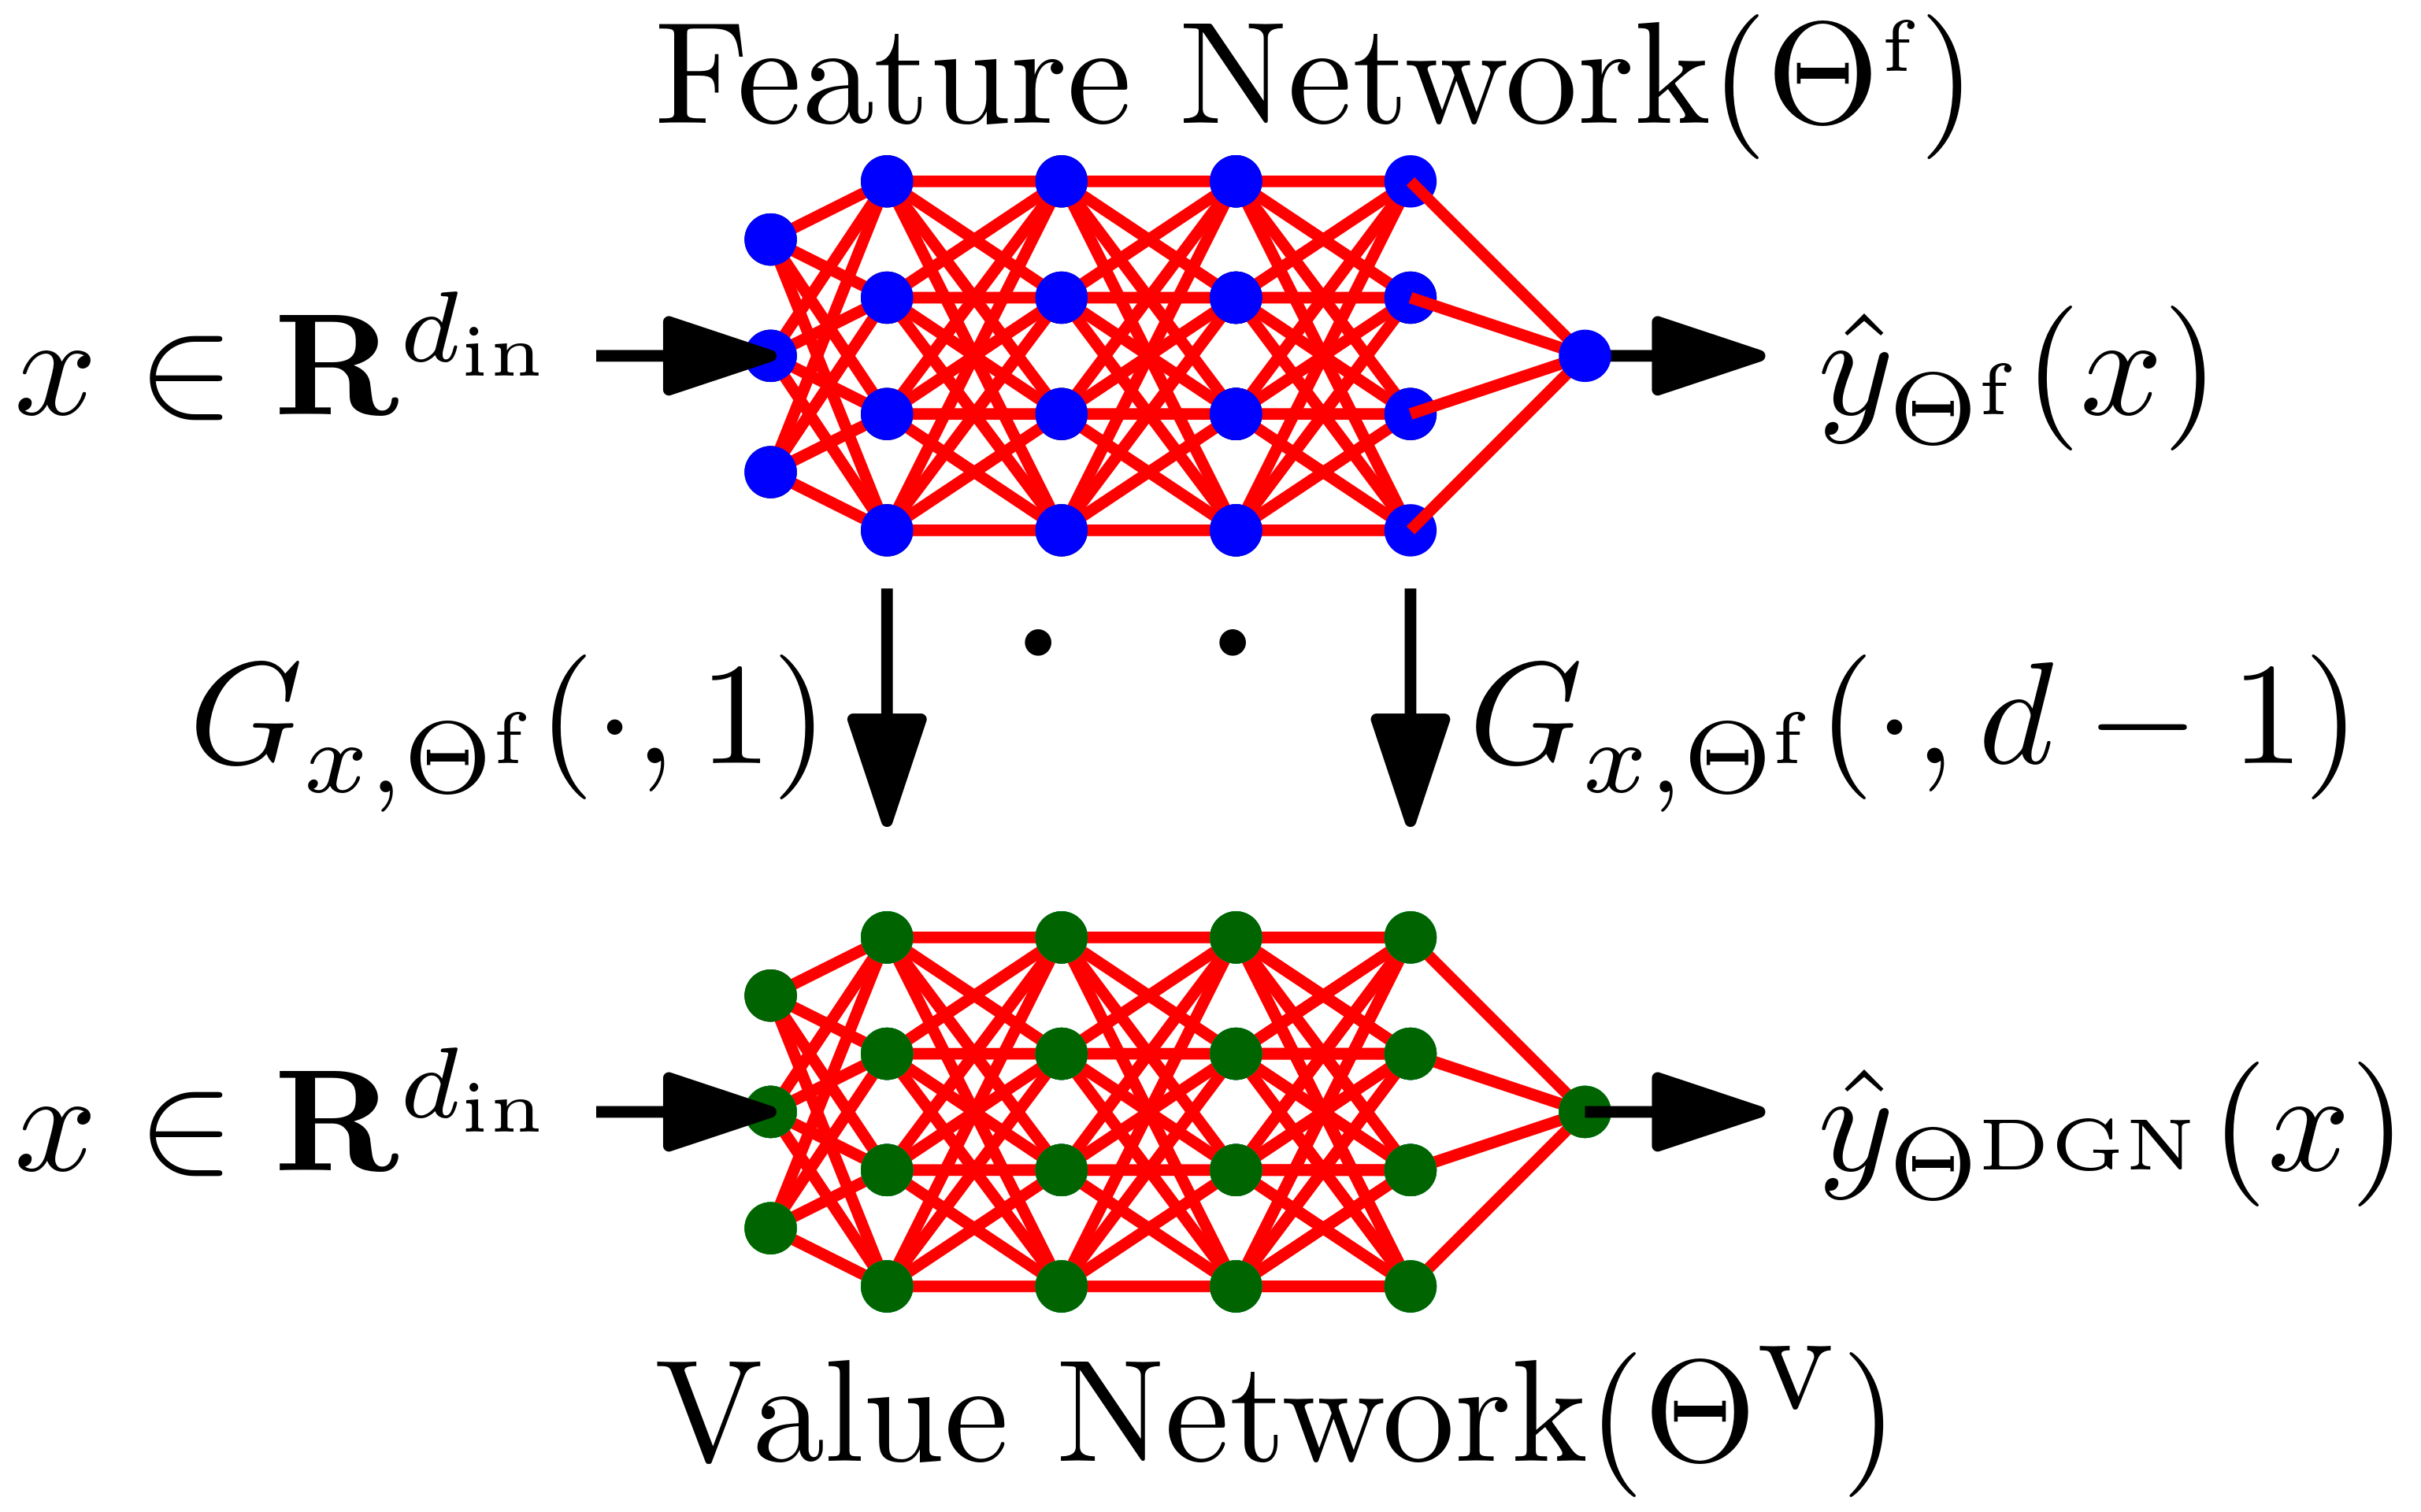
\includegraphics[scale=1]{figs/dgn-small.png}
}
\end{minipage}
\caption{\small{Shows a deep gated network (DGN). The soft-ReLU enables gradient flow into the feature network.}}
\label{fig:dgn}
\end{figure}

\textbf{DGN} set up was introduced by \citetalias{ch2020neural} to  analytically characterise the role played by the gates in a `standalone' manner. The DGN has two networks namely the \emph{feature network} parameterised by $\Tf\in\R^{d^{\text{f}}_{\text{net}}}$ which holds the NPFs (i.e., the gating information) and a \emph{value network} parameterised by $\Tv\in\R^{d^{\text{v}}_{\text{net}}}$ which holds the NPV.  The combined parameterisation is denoted by $\Theta^{\text{DGN}}=(\Tf,\Tv)\in \R^{d^{\text{f}}_{\text{net}}+d^{\text{v}}_{\text{net}}}$.  Thus the learning problem in the DGN is $\hat{y}_{\Tdgn}(x)=\ip{\phi_{x,\Tf},v_{\Tv}}$. 
% \subsection{Background: Deep Gated Networks}\label{sec:decoupled}
\begin{comment}
\begin{tabular}{lll}
Feature Network (FN) 	&:&	$\Tf\in\R^{\dfnet}$; provides the gates/masks i.e., the NPFs.\\
Value Network (VN)		&:&	$\Tv\in\R^{\dvnet}$; uses the gates/masks of FN to output $\hat{y}_{\Tdgn}(x)$.\\
Learning Problem &:& $\hat{y}_{\Tdgn}(x)=\ip{\phi_{x,\Tf},v_{\Tv}}$.
\end{tabular}
\end{comment}
\begin{comment}
\begin{wrapfigure}{r}{0.25\textwidth}
  \begin{center}
    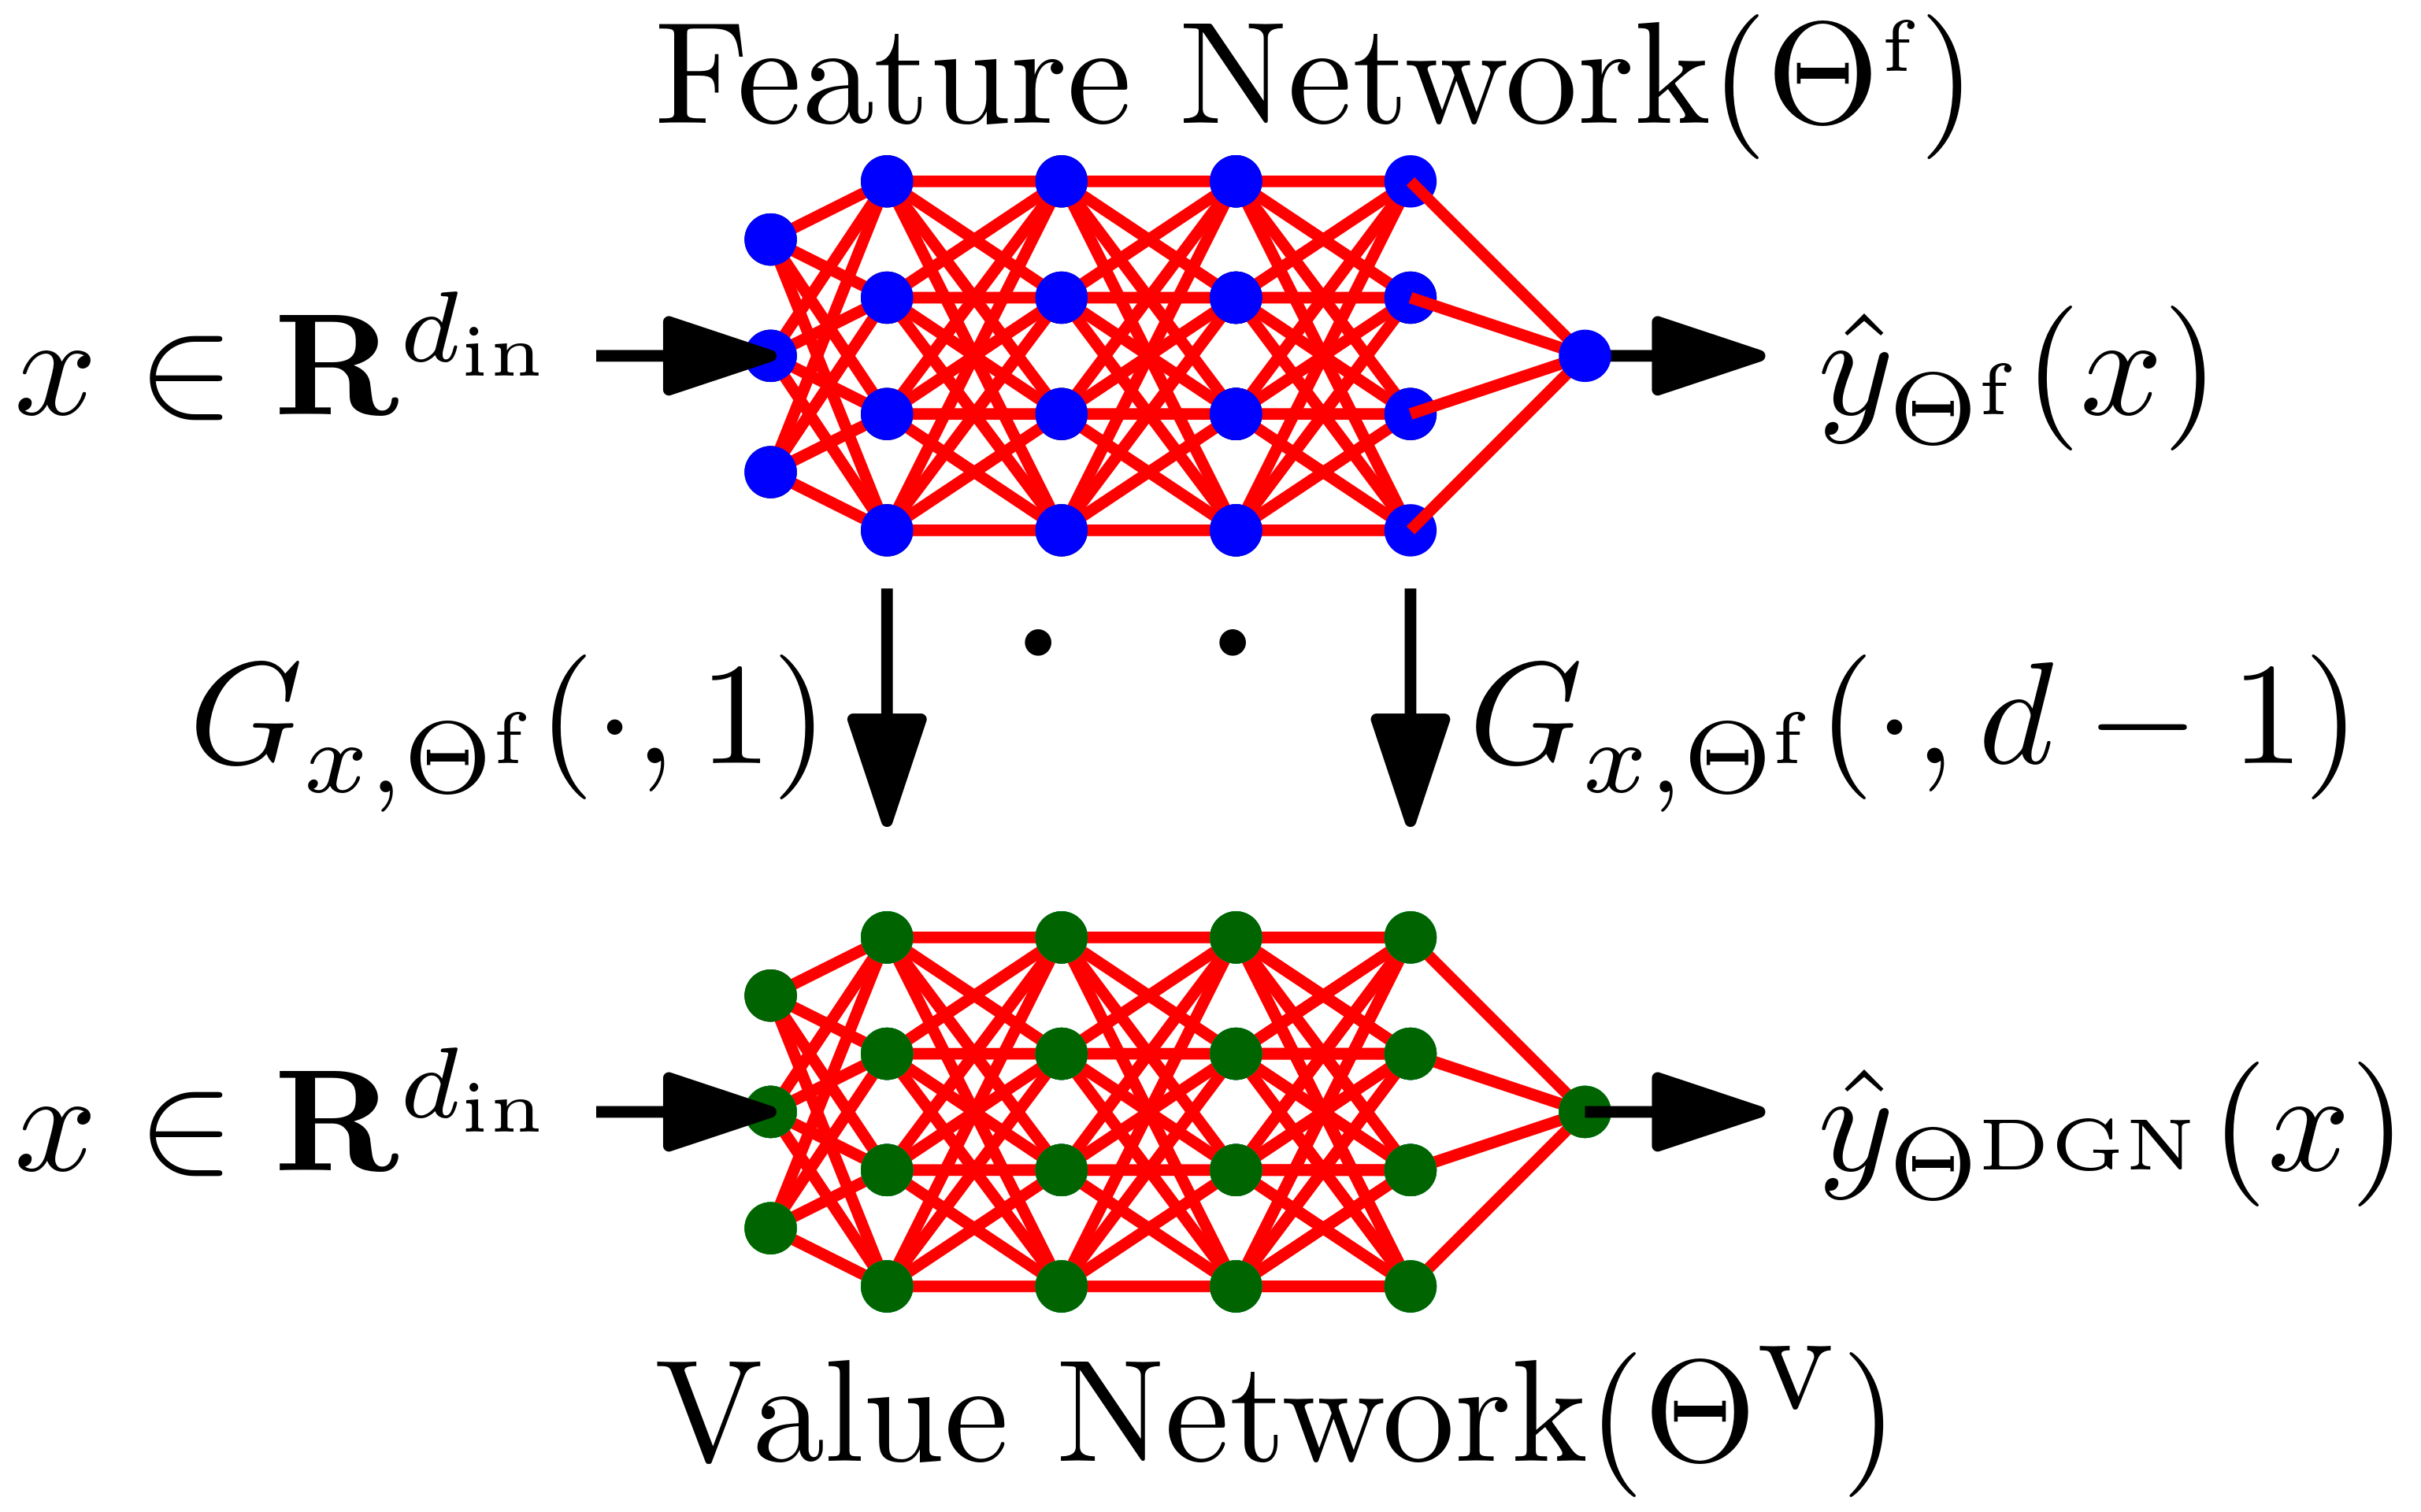
\includegraphics[width=0.25\textwidth]{figs/dgn-small.png}
  \end{center}
\caption{\small{DGN}}
\label{fig:dgn}
\end{wrapfigure}
\end{comment}
% Here the gates/`active sub-networks' are held in the feature network and are then used in the value network.
\begin{definition}\label{rm:regime}The DGN has $\mathbf{4}$ \textbf{regimes} namely \emph{decoupled learning} (DL), \emph{fixed learnt} (FL), \emph{fixed random-dependent initialisation} (FR-DI) and \emph{fixed random-independent initialisation} (FR-II). 
In all the regimes $\hat{y}_{\Tdgn}$ is the output, and $\Tv_0$ is always initialised at random and is \emph{trainable}. However, the regimes differ based on i) trainability of $\Tf$, ii) initialisation $\Tf_0$ as described below.\\
\begin{tabular}{lll}
DL              &: & $\Tf$ is trainable, and $\Tf_0$ and $\Tv_0$ are random and statistically independent,  $\beta>0$.\\
FL              &: & $\Tf$ is non-trainable, and $\Tf_0$ is pre-trained;  $\Tv_0$ is statistically independent of $\Tf_0$. \\
FR-II           &: & $\Tf$ is non-trainable, and $\Tf_0$ and $\Tv_0$ are random and statistically independent.\\
FR-DI   &:&  $\Tf$ is non-trainable, and $\Tf_0=\Tv_0$.\\
\end{tabular}
\end{definition}
\textbf{DGN Regimes:} The flexibility in a DGN is that  a) $\Tf$ can be trainable/non-trainable and b) $\Tf_0$ can be random or pre-trained using $\hat{y}_{\Tg}$ as the output (\Cref{rm:regime}). By using the DGN setup we can study the role of gates by comparing (a) learnable (DL) vs fixed gates (FL, FR-DI, FR-II), (b) random (FR-DI, FR-II) vs learnt gates (FL) and (c) dependent (FR-DI) vs independent initialisations (FR-II). In the DL regime `soft-ReLU' is chosen to enable gradient flow through the feature network.
%\end{comment}
\begin{comment}\textbf{Flattened Notation:} For a fully connected DNN of width $w$ and depth $d$, there are a total of $\ut=w(d-1)$ hidden units. Let  $q_{x,\Theta}(\iu)$, $G_{x,\Theta}(\iu)$, and $z_{x,\Theta}(\iu)$, where $\iu\in[\ut]$  denote the pre-activation, gating and output values of the $\ut$ hidden unit in the network, whose relationship is given in the left most illustration in \Cref{fig:hunit}.
\FloatBarrier
\begin{table}[h]
\resizebox{\columnwidth}{!}{
\begin{tabular}{|c|c|}\hline
Feature NTK & $\kv_{\Tdgn}(s,s')=\ip{\psiv_{x_s,\Tdgn},\psiv_{x_{s'},\Tdgn}}$, where $\psiv_{x,\Tdgn}=\nabla_{\Tv}\hat{y}_{\Tdgn}(x)\in\R^{\dvnet}$\\\hline
Value NTK & $\kf_{\Tdgn}(s,s')=\ip{\psif_{x_s,\Tdgn},\psif_{x_{s'},\Tdgn}}$, where $\psif_{x,\Tdgn}=\nabla_{\Tf}\hat{y}_{\Tdgn}(x)\in\R^{\dfnet}$\\\hline
\end{tabular}
}
\caption{Definition of NTF and NTKs for DGN used in \Cref{th:main}.}
\label{tb:defks}
\end{table}
\end{comment}

\begin{proposition}\label{prop:ntks} Let $K_{\Tdgn}$ be the NTK matrix of the DGN, then $K_{\Tdgn}=\kv_{\Tdgn}+\kf_{\Tdgn}$, with
%\FloatBarrier
\begin{table}[h]
\resizebox{\columnwidth}{!}{
\begin{tabular}{|c|c|}\hline
Overall NTK & $K_{\Tdgn}(s,s')=\ip{\psi_{x_s,\Tdgn},\psi_{x_{s'},\Tdgn}}$, where $\psi_{x,\Tdgn}=\nabla_{\Tdgn}\hat{y}_{\Tdgn}(x)\in\R^{\dnet}$\\\hline
Feature NTK & $\kv_{\Tdgn}(s,s')=\ip{\psiv_{x_s,\Tdgn},\psiv_{x_{s'},\Tdgn}}$, where $\psiv_{x,\Tdgn}=\nabla_{\Tv}\hat{y}_{\Tdgn}(x)\in\R^{\dvnet}$\\\hline
Value NTK & $\kf_{\Tdgn}(s,s')=\ip{\psif_{x_s,\Tdgn},\psif_{x_{s'},\Tdgn}}$, where $\psif_{x,\Tdgn}=\nabla_{\Tf}\hat{y}_{\Tdgn}(x)\in\R^{\dfnet}$\\\hline
\end{tabular}
}
\end{table}
\end{proposition}
\textbf{Remark:} There are two separate NTKs, each one corresponding to feature and value networks respectively. In the case of fixed regimes, $\kf=0$. 

\begin{comment}
\begin{definition}
(i) For an input $x\in\R^{d_{in}}$, define $\psif_{x,\Tdgn}=\nabla_{\Tf}\hat{y}_{\Tdgn}(x)\in\R^{\dfnet}$, and $\psiv_{x,\Tdgn}=\nabla_{\Tv}\hat{y}_{\Tdgn}(x)\in\R^{\dvnet}$.  
(ii) For  $s,s'\in[n]$ define $\kf_{\Tdgn}(s,s')=\ip{\psif_{x_s,\Tdgn},\psif_{x_{s'},\Tdgn}}$ and  $\kv_{\Tdgn}(s,s')=\ip{\psiv_{x_s,\Tdgn},\psiv_{x_{s'},\Tdgn}}$.
\end{definition} 
\end{comment}
\begin{comment}
\begin{theorem}\label{th:main} Assume (i) $\Tv_0\inrdnet$ is statistically independent of $\Tf_0$ (ii) $\Tv_0$ are i.i.d symmetric Bernoulli over $\{-\frac{\sigma}{\sqrt{w}},+\frac{\sigma}{\sqrt{w}}\}$. Then, it follows that\\
(i) $\E\left[\kv_{\Tdgn_0}\right]=d \left(\frac{\sigma^2}{w}\right)^{(d-1)} H_{\Tf_0}$, (ii) $\kv_{\Tdgn_0}\ra d \left(\frac{\sigma^2}{w}\right)^{(d-1)} H_{\Tf_0}$ as $w\ra\infty$.
\end{theorem}
\end{comment}
\begin{comment}
\begin{assumption}\label{assmp:main}
(i) $\Tv_0$ is statistically independent of $\Tf_0$ (ii) $\Tv_0$ are sampled i.i.d from symmetric Bernoulli over $\{-{\sigma},+{\sigma}\}$. For FC layers $\sigfc=\frac{\cscale}{\sqrt{w}}$, and for convolutional layers $\sigcnn=\frac{\cscale}{\sqrt{w\wconv}}$.
\end{assumption}
\end{comment}
\begin{comment}
\begin{definition}[Scaling Factors]
For $\J\in 2^{[b]}$, define $\gamma_{\text{res}}(\J)=\underset{j\in \J}\Pi \gamma^{\text{pre}}_j \cdot \underset{j'\in [b]\setminus \J}\Pi \gamma^{\text{post}}_{j'}$, $\bfc=d\cdot\sigfc^{2(d-1)}$, $\bcnn=\frac{1}{{\din}^2} (\dconv \sigcnn^{2(\dconv-1)}\sigfc^{2\dfc}+\dfc \sigcnn^{2\dconv}\sigfc^{2(\dfc-1)}$, $\bres(\J)= (|\J| +2)\dblock \sigfc^{2( (|J|+2)\dblock-1)}$.
\end{definition}
\end{comment}
\begin{comment}
\begin{theorem}\label{th:main} (i) $\Tv_0$ is statistically independent of $\Tf_0$ (ii) $\Tv_0$ are i.i.d symmetric Bernoulli over $\{-{\sigma},+{\sigma}\}$. For FC layers $\sigfc=\frac{\cscale}{\sqrt{w}}$, and for convolutional layers $\sigcnn=\frac{\cscale}{\sqrt{w\wconv}}$. As $w\ra\infty$, it follows that: 
(i) FC: $\kv_{\Tdgn_0}\ra \bfc H_{\Tf_0}$,  (ii) CNN: $\kv_{\Tdgn_0}\ra \bcnn H_{\Tf_0}$, (iii) ResNet: $\kv_{\Tdgn_0}\ra \sum_{\J\in 2^{[b]}}  \bres^{\J} H^{\J}_{\Tf_0}$, where
\resizebox{\columnwidth}{!}{
\begin{tabular}{|c|c|c|}\hline
$\bfc$& $\bcnn$&$\bres^{\J}$ \\\hline
$d\sigfc^{2(d-1)}$  & $\frac{1}{{\din}^2} \left(\dconv \sigcnn^{2(\dconv-1)}\sigfc^{2\dfc}+\dfc \sigcnn^{2\dconv}\sigfc^{2(\dfc-1)}\right)$  &$(|\J| +2)\dblock \sigfc^{2\big( (|\J|+2)\dblock-1\big)} \left(\underset{j\in \J}\Pi \gamma^{\text{pre}}_j \cdot \underset{j'\in [b]\setminus \J}\Pi \gamma^{\text{post}}_{j'}\right)^2$\\\hline
\end{tabular}
}
\end{theorem}
\end{comment}
\begin{theorem}\label{th:main} (i) $\Tv_0$ is statistically independent of $\Tf_0$ (ii) $\Tv_0$ are i.i.d symmetric Bernoulli over $\{-{\sigma},+{\sigma}\}$. Let $\sigfc=\frac{\cscale}{\sqrt{w}}$ and $\sigcnn=\frac{\cscale}{\sqrt{w\wconv}}$ for FC and convolutional layers. As $w\ra\infty$, we have: 

(ii) $\kv_{\Tdgn_0}\ra \bfc H_{\Tf_0}$, $\bfc =d \sigfc^{2(d-1)}$ for FC-DNN,

(ii) $\kv_{\Tdgn_0}\ra \bcnn H_{\Tf_0}$, $\bcnn = \frac{1}{{\din}^2} \left(\dconv \sigcnn^{2(\dconv-1)}\sigfc^{2\dfc}+\dfc \sigcnn^{2\dconv}\sigfc^{2(\dfc-1)}\right)$ for  CNN with GAP,

(iii) $\kv_{\Tdgn_0}\ra \sum_{\J\in 2^{[b]}}  \bres^{\J} H^{\J}_{\Tf_0}$, $\bres^{\J} = (|\J| +2)\dblock \sigfc^{2\big( (|\J|+2)\dblock-1\big)} \Gamma(\J)^2$ for ResNet.
%\begin{align*}
%\bcnn &= \frac{1}{{\din}^2} \left(\dconv \sigcnn^{2(\dconv-1)}\sigfc^{2\dfc}+\dfc \sigcnn^{2\dconv}\sigfc^{2(\dfc-1)}\right)\\
%\bres^{\J} &= (|\J| +2)\dblock \sigfc^{2\big( (|\J|+2)\dblock-1\big)} \left(\underset{j\in \J}\Pi \gamma^{\text{pre}}_j \cdot \underset{j'\in [b]\setminus \J}\Pi \gamma^{\text{post}}_{j'}\right)^2
%\end{align*}
\end{theorem}

$\bullet$ $\bm{\bfc,\bcnn,\bres:}$ The simplest of all is $\bfc=d\sigfc^{2(d-1)}$, where $d$ is  due the fact that there are $d$ weights in a path and in the exponent of $\sigfc$, factor $(d-1)$ arises because the gradient of a particular weight is product of all the weights in the path excluding the said weight itself, and the factor of $2$ is due to the fact that NTK is an inner product of two gradients. $\bcnn$ is similar to $\bfc$ with separate bookkeeping for the convolutional and FC layers, and $\frac{1}{\din^2}$ is due to the GAP layer. In $\bres$, the $\bfc$ for all the sub-FC-DNNs within the ResNet are scaled by the corresponding normalisation factors and summed.

%$\bullet$ $\bm{\kf}$ vs $\bm{\kv}$: T
$\bullet$ \textbf{Decoupling} In a DNN with ReLU (and FR-DI regime of DGN), NPV and NPF are not statistically independent at initialisation, i.e., \Cref{th:main} does not hold. However, the current state-of-the-art analysis \cite{ntk,arora2019exact,cao2019generalization} is in the \emph{infinite width} ($w\rightarrow\infty$) regime, wherein, the change in activations during training is  only of the order $\sqrt{\frac{1}{w}}$, which goes to $0$ as $w\ra\infty$. Hence, though assumption in \Cref{th:main} may not hold exactly, it is \emph{not a strong assumption} to fix the NPFs for the purpose of analysis. Once the NPFs are fixed, it only natural to statistically decouple the NPV from fixed NPFs (\Cref{th:main} hold in FR-II, FL and DL regimes).  %Furthermore, \Cref{assmp:main} adds strength, it brings out the relationship  NTK = constant $\times$ NPK (in \Cref{th:main}). 

$\bullet$ \textbf{Gates are Key:} In simple terms, \Cref{th:main} says that if the gates/masks are known, then the weights are expendable, a fact which we also verify in our extensive experiments.
\begin{comment}
$\bullet$ \textbf{Base Kernel:} %We now informally reason out the behaviour of the base kernel $H^{\text{lyr}}_{l,\Theta_0}$ as a function of $l$. 
For each $l$, $H^{\text{lyr}}_{l,\Theta_0}$ is an inner product of the binary features, which at randomised initialisation, for infinite width is proportional $\frac{1}2-\frac{\text{arccos}\ip{z_{x_s,\Theta_0}(\cdot,l-1),z_{x_{s'},\Theta_0}(\cdot,l-1)}}{2\pi}$. Further, due to the property of ReLU to pass only positive components, it is likely that the angle $\ip{z_{x_s,\Theta_0}(\cdot,l-1),z_{x_{s'},\Theta_0}(\cdot,l-1)}$ keeps reducing with depth and $\frac{H^{\text{lyr}}_{l,\Theta_0}(s,s')}{w}\ra\frac{1}{2},\forall s,s'\in[n]$. 
\end{comment}
\begin{comment}
$\bullet$ \textbf{Interpretability:} \Cref{th:main} shows that the gates and the active sub-networks are \emph{fundamental entities arising naturally in the NTK framework}. The NPK is \emph{interpretable} in terms of the gates and active sub-networks, while NTK is defined in terms of gradients with no such interpretation. Further,\\
\indent \quad $1.$ The role of depth is interpretable in terms of the relation between $H^{\text{fc}}$ and $H^{\text{lyr}}$, and the role of residual connections,  as well as convolutions is capture in the structure of the NPK (see \Cref{sec:npk}).\\
\indent \quad $2.$ In the light of the result in \Cref{th:main} deep learning can be interpreted as a \emph{multiple kernel learning} method. Our experiments do suggest a strong evidence that the NPKs are learnt.
\end{comment}
\begin{comment}
$\bullet$ \textbf{Finite Width:} The $w\ra\infty$ condition in \Cref{th:main} needs to hold only for the value network. For the feature network, $w\ra\infty$ instead can be achieved by copying the gates of such a DNN into the feature network of identical architecture, and repeating it $m$ times and letting $m\ra\infty$ instead. 
\end{comment}
%$\bullet$ An extension of \Cref{th:main} to ResNets and CNNs is in the appendix.






%\section{Numerical Experiments}\label{sec:exp} 
We  now show via experiments that gates indeed play a central role in deep learning. For this we use the DGN setup (\Cref{fig:ablation}) to create models in the $4$ regimes namely DL, FL, FR-II and FR-DI. In each of the $4$ regimes, we create  combinatorially many models via a) permutation of the layers when the copied from the feature to the value network, and b) setting the input to the value network to $\mathbf{1}$ (in training and testing), i.e., a tensor with all its entries to be $1$. We observe that in all the $4$ regimes, the models are robust to the combinatorial variations.

\textbf{Setup:} Datasets are MNIST and CIFAR-10. For CIFAR-10, we use \Cref{fig:ablation} with $3\times 3$  windows and $128$ filters in each layer. For MNIST, we use FC instead of the convolutional layers.  All the FC-DNNs and CNNs are trained with `\emph{Adam}'  [\citenum{adam}] (step-size $=3\cdot 10^{-4}$ , batch size $=32$). We use $\beta=10$ in the DL regime.

\textbf{Reporting of Statistics:} The results are summarised in \Cref{fig:ablation}. For FC-DNN and CNN, in each of the $4$ regimes, we train $48= 2 (\xv=x / \xv=\mathbf{1}) \times 24(\text{layer permutations})$ models. Each of these models are trained to almost $100\%$ accuracy and the test performance is taken to be the best obtained in a given run. Each of the $48$ models is run only once. In all the cases the mean and deviation are reported.
\begin{figure}[b]
\begin{minipage}{0.64\textwidth}
\resizebox{\textwidth}{!}{
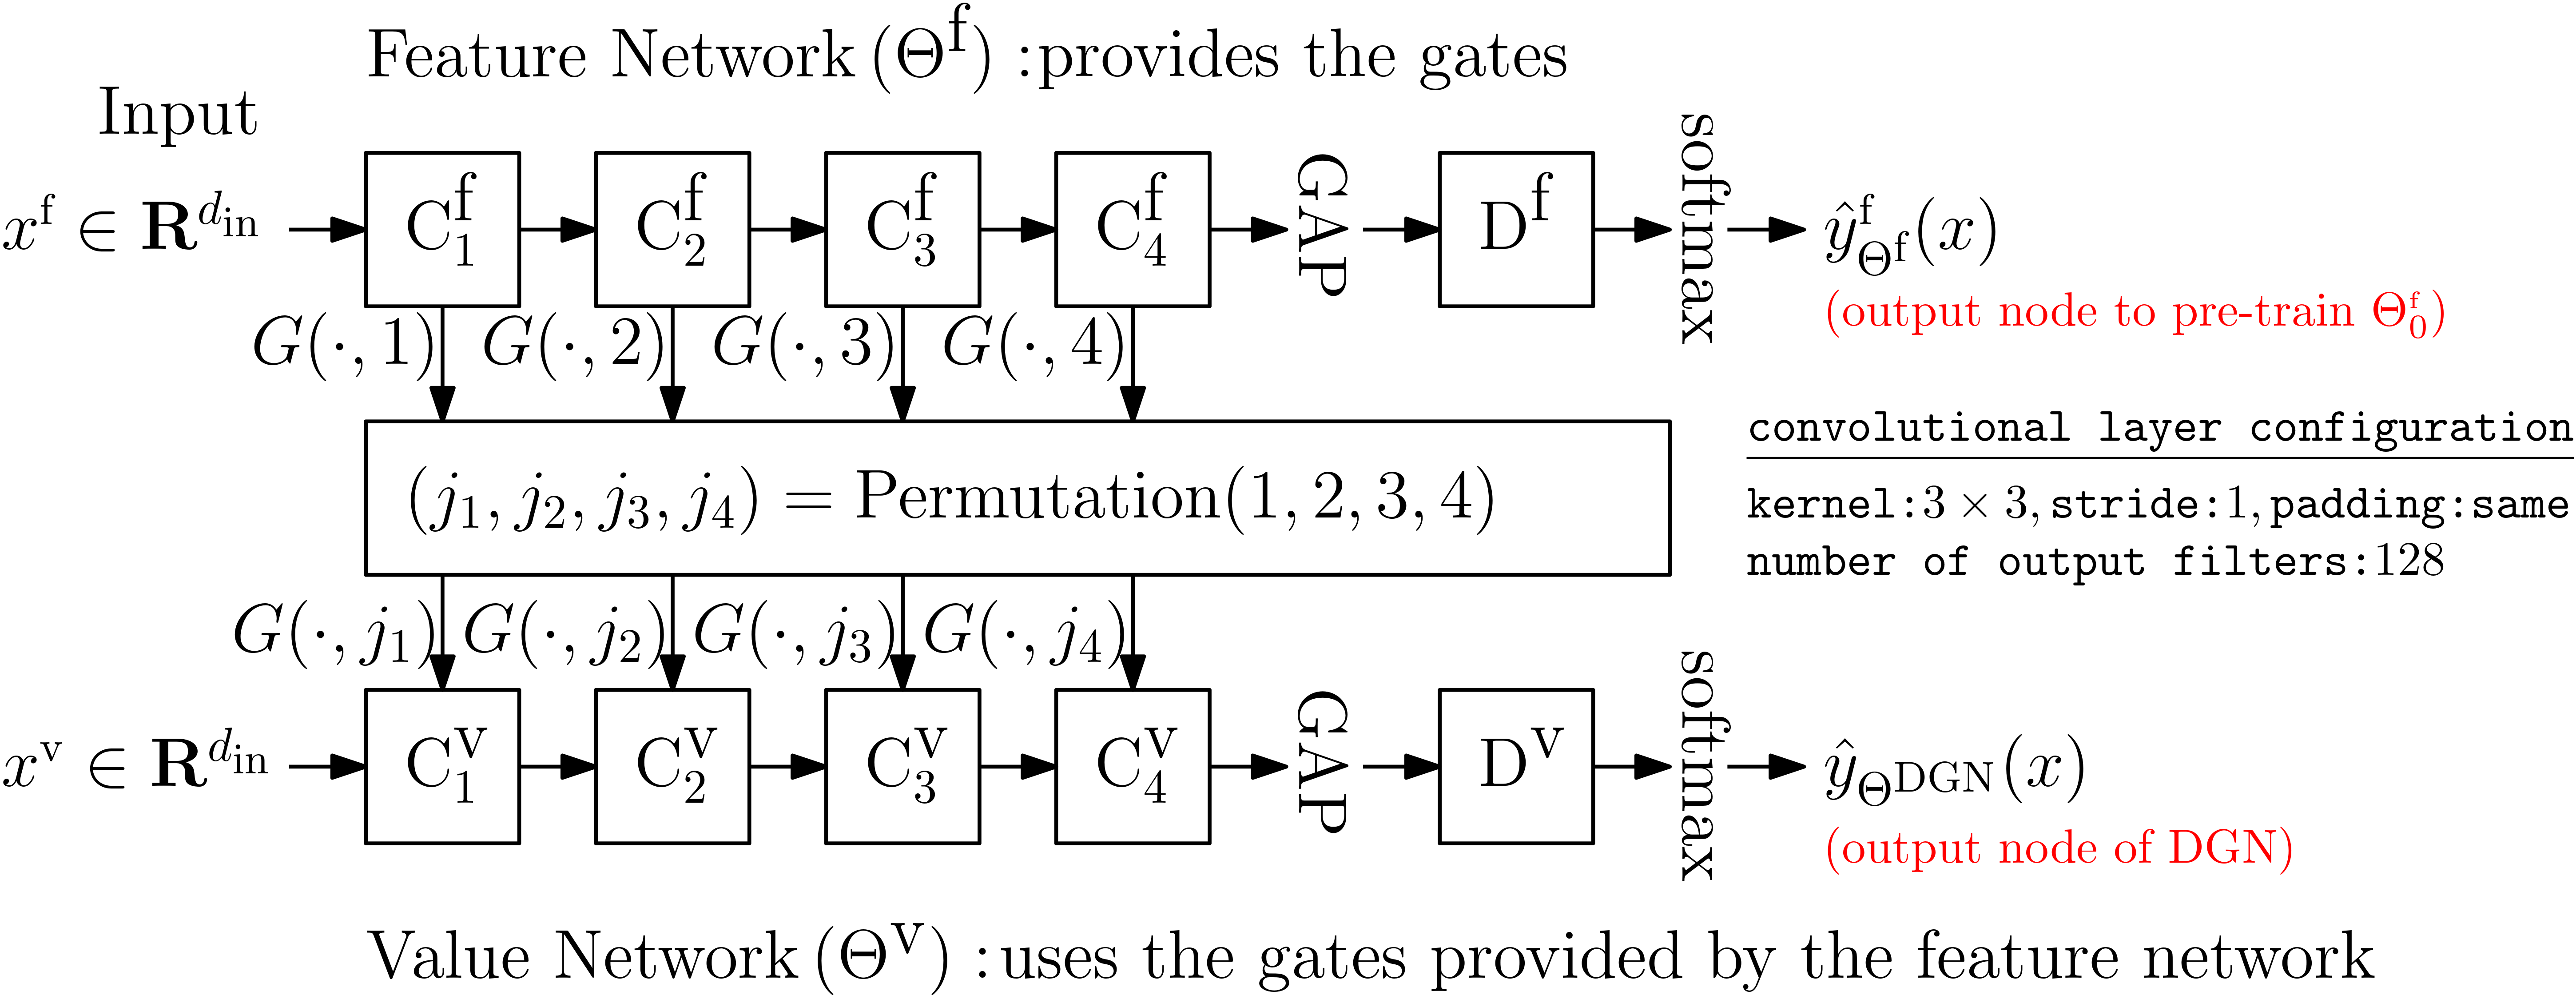
\includegraphics[scale=0.5]{figs/ablation.png}
}
\end{minipage}
\begin{minipage}{0.35\columnwidth}
\small
\resizebox{\columnwidth}{!}{
\begin{tabular}{|c|c|c|c|}\hline
&FC& CNN & ResNet\\\hline
%FR-II& $94.10\pm0.27\%$ & $67.53\pm0.73\%$\\\hline
%FR-DI& $94.06\pm0.25\%$ & $67.6\pm0.74\%$\\\hline
%DL& $98.14\pm0.07\%$ & $77.59\pm0.59\%$\\\hline
%FL& $98.62\pm0.05\%$ & $79.37\pm0.29\%$\\\hline
%ReLU& $\%$ & $\%$\\\hline
FR-II& $94.1\%$ & $67.5\%$ &$89.8\%$\\\hline
FR-DI& $94.1\%$ & $67.6\%$& $89.8\%$ \\\hline
DL& $98.1\%$ & $77.6\%$& $92.4\%$ \\\hline
FL& $98.6\%$ & $79.4\%$& $92.5\%$\\\hline
ReLU& $98.5\%$ & $80.4\%$& $93.1\%$\\\hline
\end{tabular}
}
\,In all cases, standard deviation was less than $0.5\%$. MNIST for FC, CIFAR-10 for CNN and ResNet.
\end{minipage}
\begin{comment}
\begin{minipage}{0.45\columnwidth}
\small
\resizebox{\columnwidth}{!}{
\begin{tabular}{|c|c|c|c|}\hline
& MNIST (FC)& CIFAR-10 (CNN) & CIFAR-10 (ResNet)\\\hline
%FR-II& $94.10\pm0.27\%$ & $67.53\pm0.73\%$\\\hline
%FR-DI& $94.06\pm0.25\%$ & $67.6\pm0.74\%$\\\hline
%DL& $98.14\pm0.07\%$ & $77.59\pm0.59\%$\\\hline
%FL& $98.62\pm0.05\%$ & $79.37\pm0.29\%$\\\hline
%ReLU& $\%$ & $\%$\\\hline
FR-II& $94.1\pm0.3\%$ & $67.5\pm0.7\%$ &$89.8\pm0.1\%$\\\hline
FR-DI& $94.1\pm0.3\%$ & $67.6\pm0.7\%$& $89.8\pm0.2\%$ \\\hline
DL& $98.1\pm0.1\%$ & $77.6\pm0.6\%$& $92.4\pm0.1\%$ \\\hline
FL& $98.6\pm0.1\%$ & $79.4\pm0.3\%$& $92.5\pm0.5\%$\\\hline
ReLU& $98.5\pm0.1\%$ & $80.4\pm0.3\%$& $93.1\pm0.1\%$\\\hline
\end{tabular}
}
\end{minipage}

\begin{minipage}{0.28\textwidth}
\resizebox{\columnwidth}{!}{
\begin{tabular}{|l|l|}\hline
Regimes & $\Tf$\\\hline
FR-II & R, NT\\\hline
FR-DI & R, NT, $\Tf_0=\Tv_0$\\\hline
FL & PT, NT\\\hline
DL & R, T\\\hline
\end{tabular}
}
\resizebox{\columnwidth}{!}{
\begin{tabular}{|l|l|}\hline
Mode	& Input\\\hline
Image	& $\xv=\xf=x$\\\hline
`All-Ones' & $\xf=x,\xv=\mathbf{1}$\\\hline
\end{tabular}
}
\end{minipage}
\end{comment}
\caption{\small{$\textrm{C}_i^{\text{f}},\textrm{C}_i^{\text{v}},i\in[4]$ are the convolutional layers, which are followed by \emph{global-average-pooling} (GAP) layer then by a dense layer ($\textrm{D}^{\text{f}}$/$\textrm{D}^{\text{v}}$), and a softmax layer to produce the final logits.}} %`R',  `L', `T' and `NT' stand for random, learnt, trainable and non-trainable respectively.}}
\label{fig:ablation}
\end{figure}


$\bullet$ \textbf{Result Discussion:}  Recall that in regimes FR-II and FR-DI the gates are fixed and random, and only $\Tv$ are trained. In DL regime, both $\Tf$ and $\Tv$ are trained, and FL regime $\Tf$ is pre-trained and fixed, and only $\Tv$ is trained. In the following discussion, we compare the performance of the models in various regimes, along with the performance of CNTK of \cite{arora2019exact} ($77.43\%$ in CIFAR-10) and the performance of standard DNN with ReLU.  The main observations are listed below (those by \cite{ch2020neural} are also revisited for the sake of completeness). 

\indent\quad $1.$ \emph{Decoupling:} There is no performance difference between FR-II and FR-DI.% i.e., the decoupling the gates from the weights did not affect the performance in practice. 
Further, decoupled learning of gates (DL) performs significantly better than fixed random gates (FR), and the gap between standard DNN with ReLU and DL is less than $3\%$. This marginal performance loss seems to be worthy trade off for fundamental insights of \Cref{th:main} under the decoupling assumption.


\indent\quad $2.$ \emph{Recovery:} The fixed learnt regime  (FL) shows that using the gates of a pre-trained ReLU network, performance can be recovered by training the NPV. Also, by interpreting the input dependent component of a model to be the features and the input independent component to be the weights, it makes sense to look at the gates/NPFs as the hidden features and NPV as the weights.% (which can be re-trained).

\indent\quad $3.$ \emph{Random Gates:} FR-II does perform well in all the experiments (note that for a $10$-class problem, a random classifier would achieve only $10\%$ test accuracy). Given the observation that the gates are the true features, and the fact that is no learning in the gates in the fixed regime, and the performance of fixed random gates can be purely attributed to the in-built structure.

\indent\quad $4.$ \emph{Gate Learning:} We group the models into three sets where $S_1=\{$ ReLU, FL , DL$\}$, $S_2=\{$ FR$\}$ and $S_3=\{$ CNTK $\}$, and explain the difference in performance due to gate learning.
 $S_2$ and $S_3$ have no gate learning. However,  $S_3$ due to its infinite width has better averaging resulting in a well formed kernel and hence performs better than $S_2$ which is a finite width. Thus, the difference between $S_2$ and $S_3$ can be attributed to finite versus infinite width. Both $S_1$ and $S_2$ are finite width, and hence, conventional feature learning happens in both $S_1$ and $S_2$, but, $S_1$ with gate learning is better ($77.5\%$ or above in CIFAR-10) than $S_2$ ($67\%$ in CIFAR-10) with no gate learning. Thus neither finite width, nor the conventional feature learning explain the difference between $S_1$ and $S_2$. Thus, `gate learning' discriminates the regimes $S_1, S_2$ and $S_3$ better than the conventional feature learning view.

\indent\quad $5.$ \emph{Permutation and Input Invariance:} The performance (in all the $4$ regimes) is  robust to `all-ones' inputs. Note that in the `all-ones' case, the input information affects the models only via the gates. Here, all the entries of the input Gram matrix are identical, and the NPK depends only on $\Lambda$, which is the measure of sub-network active simultaneously for the various input pairs. The performance (in all the $4$ regimes) is also robust to permutation of the layers. This can be attributed to the product $\Pi_{l=1}^{(d-1)} H^{\text{lyr}}_{l,\Theta}$ of the layer level base kernels being order invariant.

\indent\quad $6.$ \emph{Visualisation:} \Cref{fig:permute} compares the hidden layer outputs of a standard DNN with ReLU with $4$ layers, and that of a DGN which copies the gates from the standard DNN, but, reverses the gating masks when applying to the value network. Also, the value network of the DGN was provided with a fixed random input (as shown in \Cref{fig:permute}). Both the models achieved about $80\%$ test accuracy, an otherwise surprising outcome, yet, as per the theory developed in this paper, a random input to the value network should not have much effect on performance, and this experiment confirms the same.
\FloatBarrier
\begin{figure}[h]
\resizebox{\columnwidth}{!}{
\includegraphics{visual-iclr/images/horse.png}
\includegraphics{visual-iclr/images/original/layer_1_0.png}
\includegraphics{visual-iclr/images/original/layer_1_1.png}
\includegraphics{visual-iclr/images/original/layer_2_0.png}
\includegraphics{visual-iclr/images/original/layer_2_1.png}
\includegraphics{visual-iclr/images/original/layer_3_0.png}
\includegraphics{visual-iclr/images/original/layer_3_1.png}
\includegraphics{visual-iclr/images/original/layer_4_0.png}
\includegraphics{visual-iclr/images/original/layer_4_1.png}
}\\
%\tiny\text{For each model, input is shown first and then starting from the first layer, the first $2$ filters of each of the $4$ layers are shown.}
\end{figure}
\FloatBarrier
\begin{figure}[h]
\resizebox{\columnwidth}{!}{
\includegraphics{visual-iclr/images/randinput.png}
\includegraphics{visual-iclr/images/permuted/layer_1_0.png}
\includegraphics{visual-iclr/images/permuted/layer_1_1.png}
\includegraphics{visual-iclr/images/permuted/layer_2_0.png}
\includegraphics{visual-iclr/images/permuted/layer_2_1.png}
\includegraphics{visual-iclr/images/permuted/layer_3_0.png}
\includegraphics{visual-iclr/images/permuted/layer_3_1.png}
\includegraphics{visual-iclr/images/permuted/layer_4_0.png}
\includegraphics{visual-iclr/images/permuted/layer_4_1.png}
}
\end{figure}


\subsection{DGN as a Lookup Table: Applying \Cref{th:main} to a pure memorisation task}\label{sec:mem}

In this section, we modify the DGN in \Cref{fig:dgn} into a memorisation network to solve a pure memorisation task. The objective of constructing the memorisation network is to understand the roles of depth and width in \Cref{th:main} in a simplified setting. In this setting, we show increasing depth till a point helps in training and increasing depth beyond it hurts training. 

\begin{definition}[Memorisation Network/Task]
Given a set of values $(y_s)_{s=1}^n\in  \R$, a memorisation network (with weights $\Theta\in\R^{\dnet}$) accepts $s\in[n]$ as its input and produces $\hat{y}_{\Theta}(s)\approx y_s$ as its output. The loss of the memorisation network is defined as $L_{\Theta}=\frac{1}{2}\sum_{s=1}^n (\hat{y}_{\Theta}(s)-y_s)^2$.
\end{definition}
\FloatBarrier
\begin{table}[h]
\centering
\begin{tabular}{| l |  l  |}\hline
Layer&  Memorisation Network\\\hline
Input  &$z_{\Theta}(0)=1$ \\
Pre-Activation & $q_{s,\Theta}(l)=\sum_{j}\Theta(i,j,l)\cdot z_{s,\Theta}(j,l-1)$\\
Hidden & $z_{s,\Theta}(i,l)=q_{s,\Theta}(i,l)\cdot G_{s}(i,l)$ \\
Final  Output & $\hat{y}_{\Theta}(s)=\sum_{j} \Theta(1,j,d) \cdot z_{s,\Theta}(j,d-1)$\\\hline
\end{tabular}
\caption{ Memorisation Network. The input is fixed and is equal to $1$. All the internal variables depend on the index $s$ and the parameter $\Theta$. The gating values $G_s(i,l)$ are external and independent variables.}
\label{tb:dgnmemo}
\end{table}

\textbf{Fixed Random Gating:} The memorisation network is described in \Cref{tb:dgnmemo}. In a memorisation network, the gates are \emph{fixed and random}, i.e., for each index $s\in[n]$, the gating values $G_{s}(i,l),\forall l\in[d-1], i\in[w] $ are sampled from $Ber(\mu), \mu\in(0,1)$ taking values in $\{0,1\}$,  and kept fixed throughout training. The input to the memorisation network is fixed as $1$, and since the gating is fixed and random there is a separate random sub-network to memorise each target $y_s\in\R$. The memorisation network can be used to memorise the targets  $(y_s)_{s=1}^n$ by training it using gradient descent by minimising the squared loss $L_{\Theta}$. In what follows, we let $K_0$ and $H_0$ to be the NTK and NPK of the memorisation network at initialisation.


\textbf{Performance of Memorisation Network:} From \Cref{prop:basic} we know that as $w\ra\infty$, the training error dynamics of the memorisation network follows:
\begin{align}
\dot{e}_t=-K_{0} e_t,
\end{align}
i.e., the spectral properties of $K_0$ (or $H_0$) dictates the rate of convergence of the training error to $0$. In the case of the memorisation network with fixed and random gates, we can calculate $\E{K_0}$ explicitly. 

\textbf{Spectrum of $H_0$:} The input Gram matrix $\Sigma$ is a $n\times n$ matrix with all entries equal to $1$ and its rank is equal to 1, and hence $H_0=\Lambda_0$. We can now calculate the properties of $\Lambda_0$. It is easy to check that $\mathbb{E}_{\mu}\left[\Lambda_0(s,s)\right]=(\mu w)^{(d-1)},\forall s\in[n]$ and $\mathbb{E}_{\mu}\left[\Lambda_0(s,s')\right]=(\mu^2 w)^{(d-1)},\forall s,s'\in[n]$.  For $\sigma=\sqrt{\frac{1}{\mu w}}$, and $\mathbb{E}_{\mu}\left[K_0(s,s)/d\right]=1$, and $\mathbb{E}_{\mu}\left[K_0(s,s')/d\right]=\mu^{(d-1)}$. 
\begin{figure}
\centering
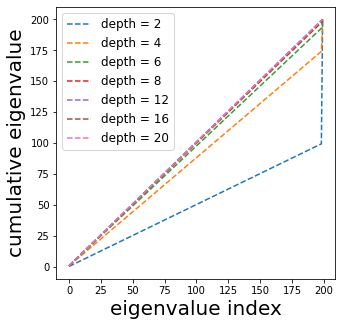
\includegraphics[scale=0.3]{figs/dgn-fra-ecdf-ideal-small.png}
\caption{Ideal spectrum of $\E{K_0}/d$ for a memorisation network for $n=200$.}
\label{fig:ideal-spectrum}
\end{figure}


\textbf{Why increasing depth till a point helps ?} 
We have:
%\comment{
\begin{align}\label{eq:mat}
\frac{\E{K_0}}{d}=\left[\begin{matrix}
1 &\mu^{d-1} &\ldots &\mu^{d-1} &\ldots\\ 
\ldots &1 &\ldots &\mu^{d-1} &\ldots\\ 
\ldots &\mu^{d-1} &\ldots &1 &\ldots \\
\ldots &\mu^{d-1} &\ldots &\mu^{d-1} &1\\ 
\end{matrix}\right]
\end{align}
%}
i.e., all the diagonal entries are $1$ and non-diagonal entries are $\mu^{d-1}$. Now, let $\rho_i\geq 0,i \in [n]$ be the eigenvalues of $\frac{\E{K_0}}{d}$, and let $\rho_{\max}$ and $\rho_{\min}$ be the largest and smallest eigenvalues.  One can easily show that $\rho_{\max}=1+(n-1)\mu^{d-1}$ and corresponds to the eigenvector with all entries as $1$, and $\rho_{\min}=(1-\mu^{d-1})$ repeats $(n-1)$ times,  which corresponds to eigenvectors given by $[0, 0, \ldots, \underbrace{1, -1}_{\text{$i$ and $i+1$}}, 0,0,\ldots, 0]^\top \in \R^n$ for $i=1,\ldots,n-1$. Note that as $d\ra\infty$, $\rho_{\max},\rho_{\min}\ra 1$.

\textbf{Why increasing depth beyond a point hurts?} 
As the depth increases the variance of the entries $K_0(s,s')$ deviates from its expected value $\E{K_0(s,s')}$. Thus the structure of the Gram matrix degrades from \eqref{eq:mat}, leading to smaller eigenvalues.
%\FloatBarrier
\begin{figure}
\resizebox{\textwidth}{!}{
\begin{tabular}{cccc}
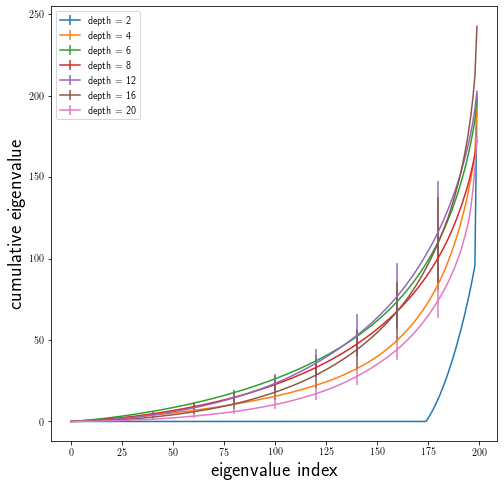
\includegraphics[scale=0.5]{figs/dgn-fra-ecdfbyd-w25.png}
&
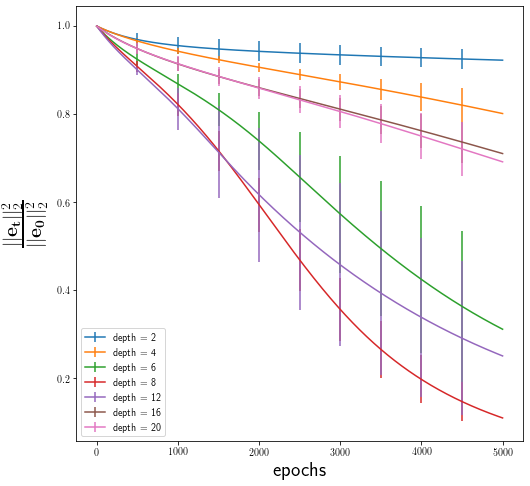
\includegraphics[scale=0.5]{figs/dgn-fra-conv-w25.png}
&
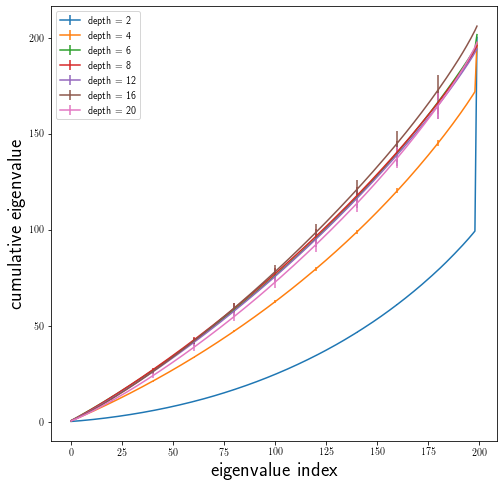
\includegraphics[scale=0.5]{figs/dgn-fra-ecdfbyd-w500.png}
&
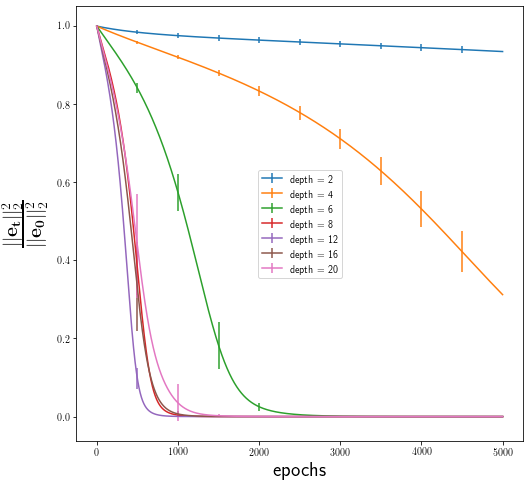
\includegraphics[scale=0.5]{figs/dgn-fra-conv-w500.png}
\end{tabular}
}
\caption{Shows the plots for the memorisation network with $\mu=\frac{1}{2}$ and $\sigma=\sqrt{\frac{2}{w}}$. The number of points to be memorised is $n=200$. The left most plot shows the e.c.d.f for $w=25$ and the second plot from the left shows the error dynamics during training for $w=25$. The second plot from the right shows the e.c.d.f for $w=500$ and the right most plot shows the error dynamics during training for $w=500$. All plots are averaged over $10$ runs.}
\label{fig:dgn-frg-gram-ecdf}
\end{figure}

\subsection{Experiment}
We set $n=200$, and $y_s\sim\text{Uniform}[-1,1]$. We look at the cumulative eigenvalue (e.c.d.f) obtained by first sorting the eigenvalues in ascending order then looking at their cumulative sum. The ideal behaviour (\Cref{fig:ideal-spectrum}) as predicted from theory is that for indices $k\in[n-1]$, the e.c.d.f should increase at a linear rate, i.e., the cumulative sum of the first $k$ indices is equal to $k(1-\mu^{d-1})$, and the difference between the last two indices is $1+(n-1)\mu^{d-1}$. In \Cref{fig:dgn-frg-gram-ecdf}, we plot the actual e.c.d.f for various depths $d=2,4,6,8,12,16,20$ and $w=25,500$ (first and third plots from the left in \Cref{fig:dgn-frg-gram-ecdf}). 

\textbf{Roles of depth and width:} In order to compare how the rate of convergence varies with the depth, we set the step-size $\alpha=\frac{0.1}{\rho_{\max}}$, $w=100$. We use the vanilla SGD-optimiser. Note the$ \frac{1}{\rho_{\max}}$ in the stepsize, ensures that the uniformity of maximum eigenvalue across all the instances, and the convergence should be limited by the smaller eigenvalues. We also look at the convergence rate of the ratio $\frac{\norm{e_t}^2_2}{\norm{e_0}^2_2}$. We notice that for $w=25$, increasing depth till $d=8$ improves the convergence, however increasing beyond $d=8$ worsens the convergence rate. For $w=500$, increasing the depth till $d=12$ improves convergence, and $d=16,20$ are worse than $d=12$.  %This matches with the depth phenomena observed in practical DNNs and also matches our theory.

%\section{Other Related Works and Future Work}
We are primarily interested in a pedagogical nugget that helps us to interpret DNNs with ReLU. The main takeaway from duality \cite{npk} was most information is stored in the gates, which is characterised by the NPK. In this paper we further simplified the NPK to reveal for the first time literature additional properties such as invariance to layer permutations and constant inputs which were also verified experimentally. We have thus strengthened the view that gates are more important. Since learning in the gates takes the NPK/NTK significantly away from the randomised initialisation, a natural direction aligned with our work would be to understand how learning in gate happens, as opposed to a design and analysis based on kernels at randomised initialisation \cite{disentangling,nth,meanres,deepres,spectra,laplace,belkin,label,fcgp,convgp}. The following are interesting future directions:

1)  Analysing learning in NPFs/gates seems to be an important problem. However, it is also a difficult problem to tackle in the case of DNNs with ReLU due to the fact that both NPFs and NPV are coupled. Our experiments showed that the DGN as a standalone network with learning of the gates (in DL regime) matches the performance of standard DNNs within $3\%$. Since in a DGN, the NTK$=\text{NTK}^{\text{fixed-gate}}+\text{NTK}^{\text{gate-learn}}$, it will be an interesting direction (and perhaps easier) to study $\text{NTK}^{\text{gate-learn}}$, which is related to learning in gates. 

2) Another direction is to look at the constant input experiment from an adversarial example standpoint: since the input to value network is a constant, the adversary can only attack via the feature network, i.e., the gates.  

3) It will also be interesting to investigate the practical benefits of the sum of product structure in ResNet.

\section{Conclusion}
In this paper, we proposed a \emph{pedagogical nugget} based on duality and neural tangent kernel, which provided a simplified understanding of deep neural networks with rectified linear units. Using this we explained/interpreted roles of activation, weights, depth, width, skip connections and convolutions with pooling in a simple manner. Based on our theory, we also showed empirically that permuting the layers or providing constant input does not degrade performance. The results (theoretical and empirical) strengthened the view that gates are more important. We concluded by pointing out some future directions, of which understanding the learning in the gates is of primary importance.



\begin{comment}
Learning in gates is also takes away the importance of looking at NPK at randomised initialisation, a reason why we did not pursue the question of analysing the spectrum of NPK at randomised initialisation in the limit of infinite width/depth (like \cite{disentangling,spectra}) or design a pure kernel method (like \cite{arora2019,fcgp,convgp}) or its constancy as in \cite{belkin}. The NTK and NPFs are related at an algebraic level (see \Cref{prop:ntknew}), i.e., the relation holds for any width, depth, and initialisation, and not just in limiting case. Also, our result that convolutions with pooling make the NPFs rotationally invariant is again algebraic and holds for finite width/depth as opposed to an asymptotic analytical characterisation of pooling \cite{disentangle}. Similarly, the sum of product structure of ResNets is also an algebraic result as opposed to \cite{meanres} which shows that ResNets are an ensemble of shallow architecture by ignoring certain higher order terms in the mean-field analysis. \cite{loss} study the dynamics of NTK empirically and show that its performance matches that of full network training in $15\%$ to $45\%$ of training time. The fact that NPF/NPK/gates learning is continuous ($\text{NTK}^{\text{gate-learn}}$ dictates the dynamics of the gates) and that learnt NPF/NPK/gates perform as well as the original DNN was already empirically shown by \cite{npk}, and our experiments add strength for the same. 

Several recent works \cite{disentangling,nth,meanres,deepres,spectra,laplace,belkin,loss} have looked at the NTK. We are primarily interested in a pedagogical nugget that helps us to interpret DNNs with ReLU. Our work is based on duality \cite{npk} which differs at a conceptual level from the aforementioned works in the following ways: (i) firstly the role of ReLU is explicitly accounted by encoding them as NPFs, (ii) the connection between the NTK and NPF is algebraic (see \Cref{prop:ntknew}) and not just in the limiting case (iii) as per theory (\Cref{th:main}) so long as the weights of the value network are random and statistically decoupled from NPFs, the NPV do not play an important role and a fact which is also verified experimentally where using the NPFs alone the NPV could be trained from scratch (iv) the NPK can correspond to arbitrary finite width feature network weights (see remark on role of activations in \Cref{sec:fc}) and not just random.  Our experiments (as well as those by \cite{npk}) showing that learning in the gates is the difference between NTK and finite width DNNs is the key differentiator from \cite{nth,label} which also looked at difference between finite width DNNs and NTK. The learning in gates is also takes away the importance of looking at NPK at randomised initialisation, a reason why we did not pursue the question of analysing the spectrum of NPK at randomised initialisation in the limit of infinite width/depth (like \cite{disentangling,spectra}) or design a pure kernel method (like \cite{arora2019,fcgp,convgp}) or its constancy as in \cite{belkin}. Further, we believe that the NPK at randomised initialisation might also be associated with a simpler kernel in manner to the result that (\cite{laplace}) NTK for FC-DNN with ReLU  is closely related to the standard Laplace kernel. Our result that convolutions with pooling make the NPFs rotationally invariant is again algebraic and holds for finite width/depth as opposed to an asymptotic analytical characterisation of pooling \cite{disentangle}. Similarly, the sum of product structure of ResNets is also an algebraic result as opposed to \cite{meanres} which shows that ResNets are an ensemble of shallow architecture by ignoring certain higher order terms in the mean-field analysis. \cite{loss} study the dynamics of NTK empirically and show that its performance matches that of full network training in $15\%$ to $45\%$ of training time. The fact that NPF/NPK/gates learning is continuous ($\text{NTK}^{\text{gate-learn}}$ dictates the dynamics of the gates) and that learnt NPF/NPK/gates perform as well as the original DNN was already empirically shown by \cite{npk}, and our experiments add strength for the same. 


\cite{disentangling} (via a spectral analysis of the NTK) show presence of (i) ordered phase, in which the trainability of DNNs degrades at large depths, but their ability to generalise does not and (ii) chaotic phase, in which, trainability improves with depth, but generalisation degrades,  (iii)  pooling  improves the depth over which networks can generalise in the chaotic phase but reduces the depth in the ordered phase. \cite{spectra} show that the eigenvalue distributions of the Conjugate Kernel and Neural Tangent Kernel converge to deterministic limits. In order to explain the difference between the NTK and finite width DNNs, \cite{nth} derive an infinite hierarchy of differential equations known as the neural tangent hierarchy (NTH).  \cite{label} observe that the performance gap between NTK and finite width DNN may be be partly due to the label agnostic nature of the NTK and introduce a novel approach from the perspective of label-awareness to reduce this gap. \cite{meanres} use mean-field analyses of two-layer DNNs to propose several novel training schemes for ResNets that performs well on the standard datasets. \cite{deepres} compare the kernel of deep ResNets with that of deep FFNets and show that the class of functions induced by the kernel of i) FFNets degenerates asymptotically with depth and i) ResNets does not degenerate with depth. \cite{loss} study the dynamics of NTK and show that there is a highly chaotic rapid initial transient phase in which NTK changes rapidly, followed by a phase where the NTK changes at constant velocity, and its performance matches that of full network training in $15\%$ to $45\%$ of training time. \cite{genntk} provide a generalised NTK analysis and show that noisy gradient descent with weight decay can still exhibit a “kernel-like” behaviour. \cite{belkin} show that constancy of the NTK results from the scaling properties of the norm of the Hessian matrix of the network as a function of the network width. \

\textbf{Related to NTK:} \cite{disentangling} (via a spectral analysis of the NTK) show presence of (i) ordered phase, in which the trainability of DNNs degrades at large depths, but their ability to generalise does not and (ii) chaotic phase, in which, trainability improves with depth, but generalisation degrades,  (iii)  pooling  improves the depth over which networks can generalise in the chaotic phase but reduces the depth in the ordered phase. 
\cite{scaling}  propose a theory for infinite width DNNs that connects  mean-field (MF) and constant kernel (NTK) limits. \cite{ntkregression} analyse the high-dimensional asymptotic generalisation performance of kernel regression with the NTK of a single hidden-layer neural network.



 \textbf{Gates and Sub Networks:} \cite{srivastava2014understanding} analysed the role of gates empirically and via a t-SNE based analysis showed that ``subnetworks active for examples of the same class are much more similar to each other compared to the ones activated for the examples of different classes''. They also observe gates flip which is upto $20\%$ of examples in the initial phases of training but quickly settle down to $5\%$. \cite{subnet1}, study active sub-networks at sample level and class level to propose two adversarial example detection methods.

\textbf{Our Work:} In contrast to aforementioned works on NTK, the focus of this paper has been on the NPK which is based on the gates, and instead of a pure kernel method, we use the intuition obtained on the NPK to test a finite width DGN. Further, we believe that the dual view based interpretation is more direct (such as rotational invariance of NPK due to convolutions and pooling, a fact not noticed in prior work). Our empirical results are closely tied to the theory we develop which is absent in prior empirical works that analysed the role of gates and sub-networks.
\end{comment}







\bibliographystyle{plainnat}
\bibliography{refs}
%%\section{Neural Path Framework For CNN}\label{sec:cnpf}
\textbf{Indexing:} The weights of layers $l\in[\dc]$ are denoted by $\Theta(\icin,\iin,\iout,l)$ and for layers $l\in[\dfc]+\dc$ are denoted by $\Theta(\iin,\iout,l)$. The pre-activations, gating and hidden unit outputs are denoted by $q_{x,\Theta}(\ifout,\iout,l)$,  $G_{x,\Theta}(\ifout,\iout,l)$, and $z_{x,\Theta}(\ifout,\iout,l)$ for layers $l=1,\ldots, \dc$. $\iin$ and $\iout$ are used to index the input and the output filters. $\ifout$ is used to denote the index of hidden unit (in the feature dimension) within the input and output filters. %Here, $\icin\in[\wconv]$, for $l=1\ldots,\dc$, $\iin\in[w]$ for $l=\dc+2,\ldots,\dc+\dfc+1$, $\ifin \in[1]$ for $l=1$, $\ifin \in[w]$ for $l=2,\ldots,\dc$, $\iout\in[w]$ for $l=1\ldots,\dc, \dc+2,\ldots, \dc+\dfc$,  $\iout\in[1]$ for $l=\dc+\dfc+1$, $\ifout\in[w]$ for $l=1,\ldots,\dc$.
\begin{comment}
\FloatBarrier
\begin{table}[h]
\centering
\begin{tabular}{|c|ll|}\hline
Index & Range&\\\hline
\multirow{2}{*}{$\iin$} & $\in[\din]$ & for $l=1\ldots,\dc$\\ \cline{2-3}
&$\in[w]$ & for $l=\dc+2,\ldots,\dc+\dfc+1$\\ \hline
\multirow{2}{*}{$\ifin$} & $\in[1]$ & for $l=1$\\ \cline{2-3}
&$\in[w]$ &for $l=2,\ldots,\dc$\\ \hline
\multirow{2}{*}{$\iout$} & $\in[w]$ &for $l=1\ldots,\dc, \dc+2,\ldots, \dc+\dfc$\\ \cline{2-3}
&$\in[1]$ &for $l=\dc+\dfc+1$\\ \hline
{$\ifout$} & $\in[w]$ &for $l=1,\ldots,\dc$\\ \hline
\end{tabular}
\end{table}
\end{comment}

\textbf{Shapes:} \Cref{fig:shape-main} shows the shapes of the tensors in the convolutional layers of a $1$-dimensional circular CNN considered in this paper. Here, the input is a $1$-dimensional tensor given by $x\in\R^{\din}$. The hidden nodes in a given convolutional layer have a $2$-dimensional shape of $\din\times w$, where $w$ is the number of filters in the layer. The weights of a given convolutional layer have $3$-dimensional shape of $\wconv\times w\times w$,  where $w\times w$ is because of the number of input filters times the number of output filters.
\FloatBarrier
\begin{figure}[h]
\centering
%\resizebox{\columnwidth}{!}{
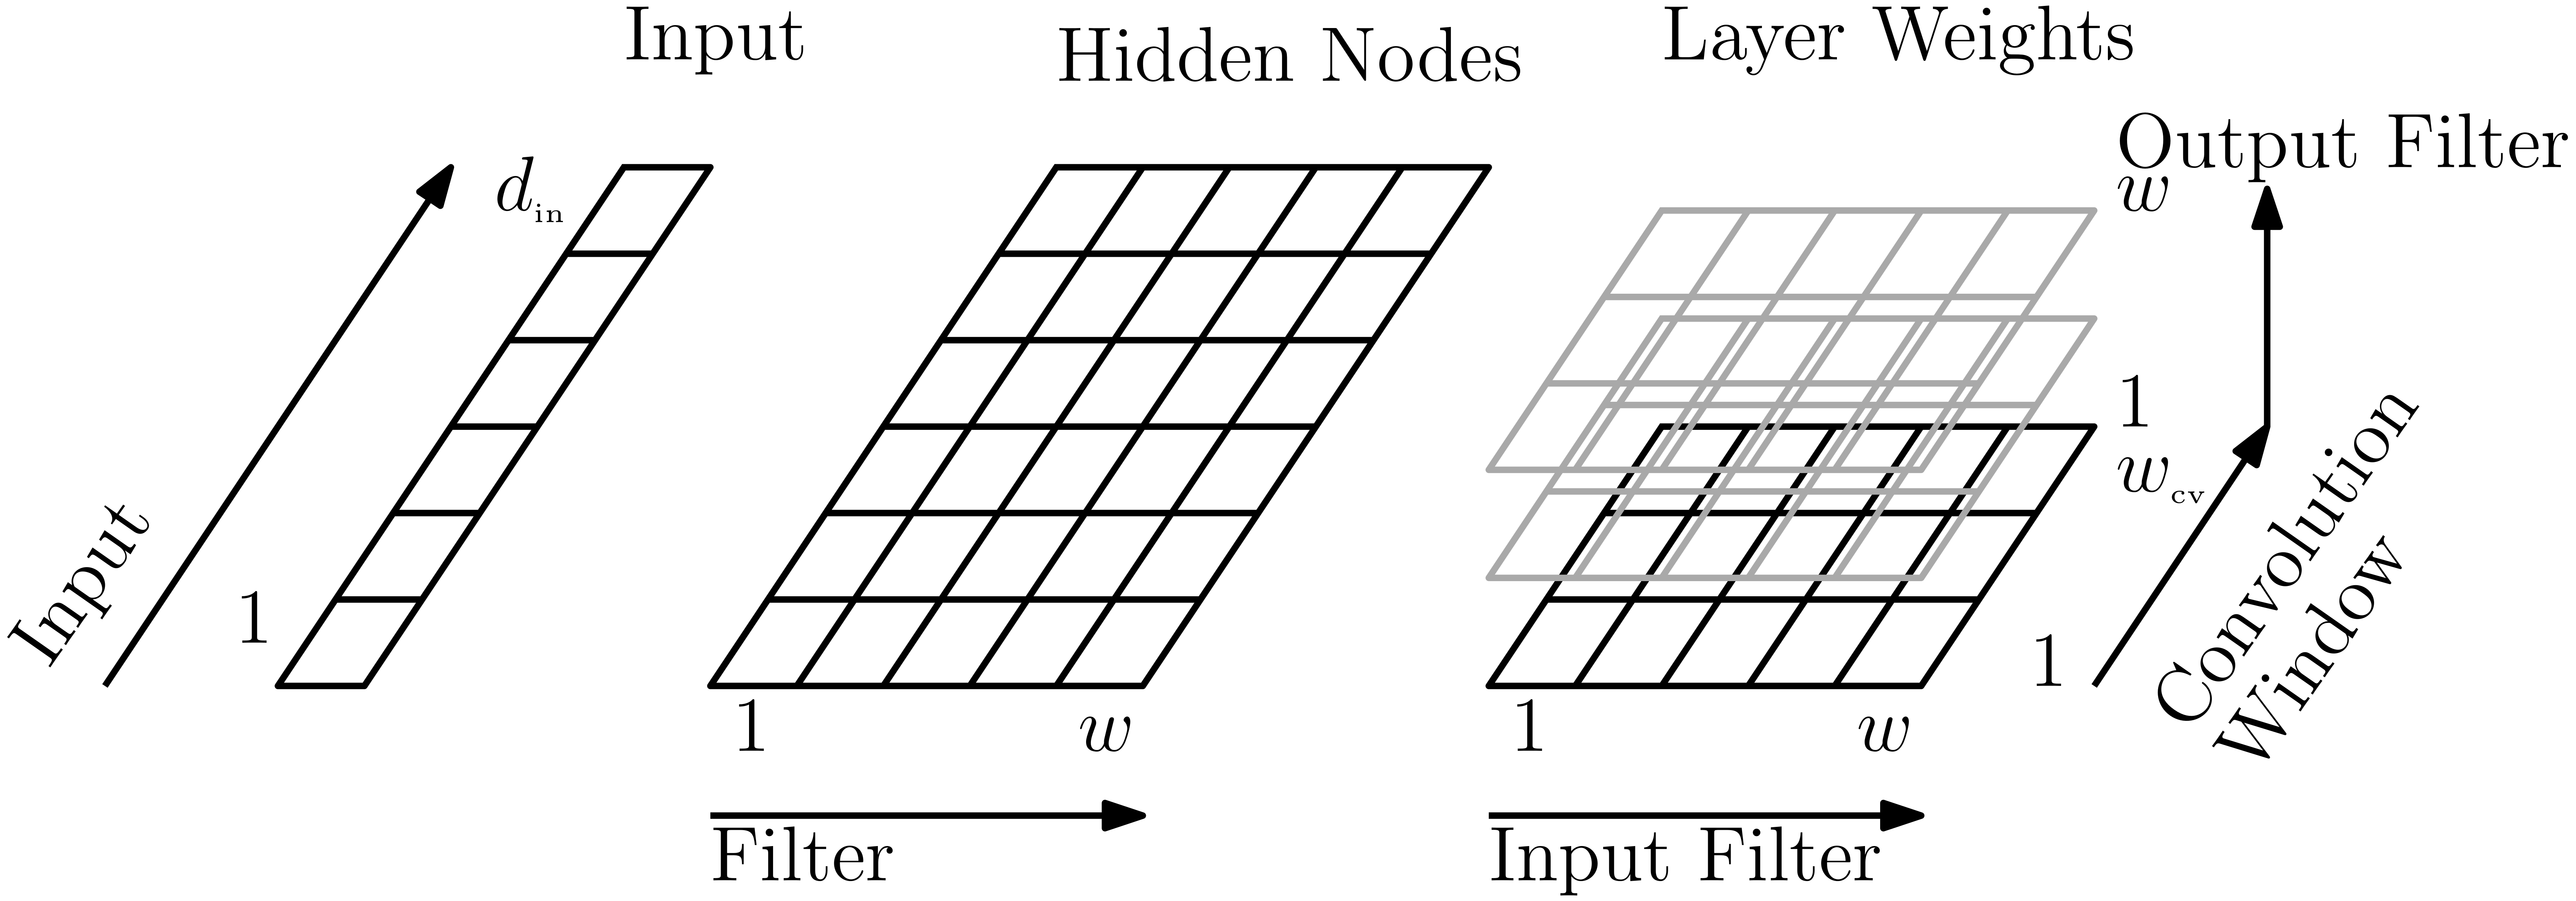
\includegraphics[scale=0.04]{figs/shape.png}
%}
\label{fig:shape-main}
\caption{Shows the shape of the tensor.}
\end{figure}

\subsubsection{Information Flow}
\begin{table}[h]
\centering
\begin{tabular}{|c l lll|}\hline
IL&: &$z_{x,\Theta}(\cdot,1,0)$ &$=$ &$x$ \\\hline\hline
\multicolumn{5}{|l|}{Convolutional Layers, $l\in[\dc]$}\\\hline\hline
PA&: & $q_{x,\Theta}(\ifout,\iout,l)$& $=$ & $\sum_{\icin,\iin}\Theta(\icin,\iin,\iout,l)\cdot z_{x,\Theta}(\ifout\oplus (\icin-1),\iin,l-1)$\\
GV&: &$G_{x,\Theta}(\ifout,\iout,l)$& $=$ & $\mathbf{1}_{\{q_{x,\Theta}(\ifout,\iout,l)>0\}}$\\
HUO&: &$z_{x,\Theta}(\ifout,\iout,l)$ & $=$ & $q_{x,\Theta}(\ifout,\iout,l)\cdot G_{x,\Theta}(\ifout,\iout,l)$\\\hline\hline
\multicolumn{5}{|l|}{GAP Layers, $l=\dc+1$}\\\hline\hline
%HUO&: &${z}_{x,\Theta}(\iout,l)$ & $=$ & $\frac{1}{\din}\sum_{i\in [\din]} z_{x,\Theta}(i,\iout,l-1)$\\\hline\hline
HUO&: &$z_{x,\Theta}(\iout, \dc+1)$ & $=$ &$\sum_{\ifout} z_{x,\Theta}(\ifout,\iout,\dc)\cdot G^{\text{pool}}_{x,\Theta}(\ifout,\iout,\dc+1)$\\\hline\hline
\multicolumn{5}{|l|}{Fully Connected Layers, $l\in[\dfc]+(\dc+1)$}\\\hline\hline
PA&: & $q_{x,\Theta}(\iout,l)$& $=$ & $\sum_{\iin}\Theta(\iin,\iout,l) \cdot z_{x,\Theta}(\iin,l-1) $\\
GV&: &$G_{x,\Theta}(\iout,l)$& $=$ & $\mathbf{1}_{\{(q_{x,\Theta}(\iout,l))>0\}}$\\
HUO&: &$z_{x,\Theta}(\iout,l)$ & $=$ & $q_{x,\Theta}(\iout,l)\cdot G_{x,\Theta}(\iout,l)$\\
FO&: & $\hat{y}_{\Theta}(x)$ & $=$ & $\sum_{\iin}\Theta(\iin,\iout, d)\cdot z_{x,\Theta}(\iin,d-1)$\\\hline
\end{tabular}
\caption{Here IL, PA, GV, HUO, GL and FO are abbreviations for input layer, pre-activation, gating values, hidden unit output, GAP-layer and final output respectively.}
\label{tb:cconv}
\end{table}

\FloatBarrier
\begin{figure}[H]
\centering
\resizebox{\columnwidth}{!}{
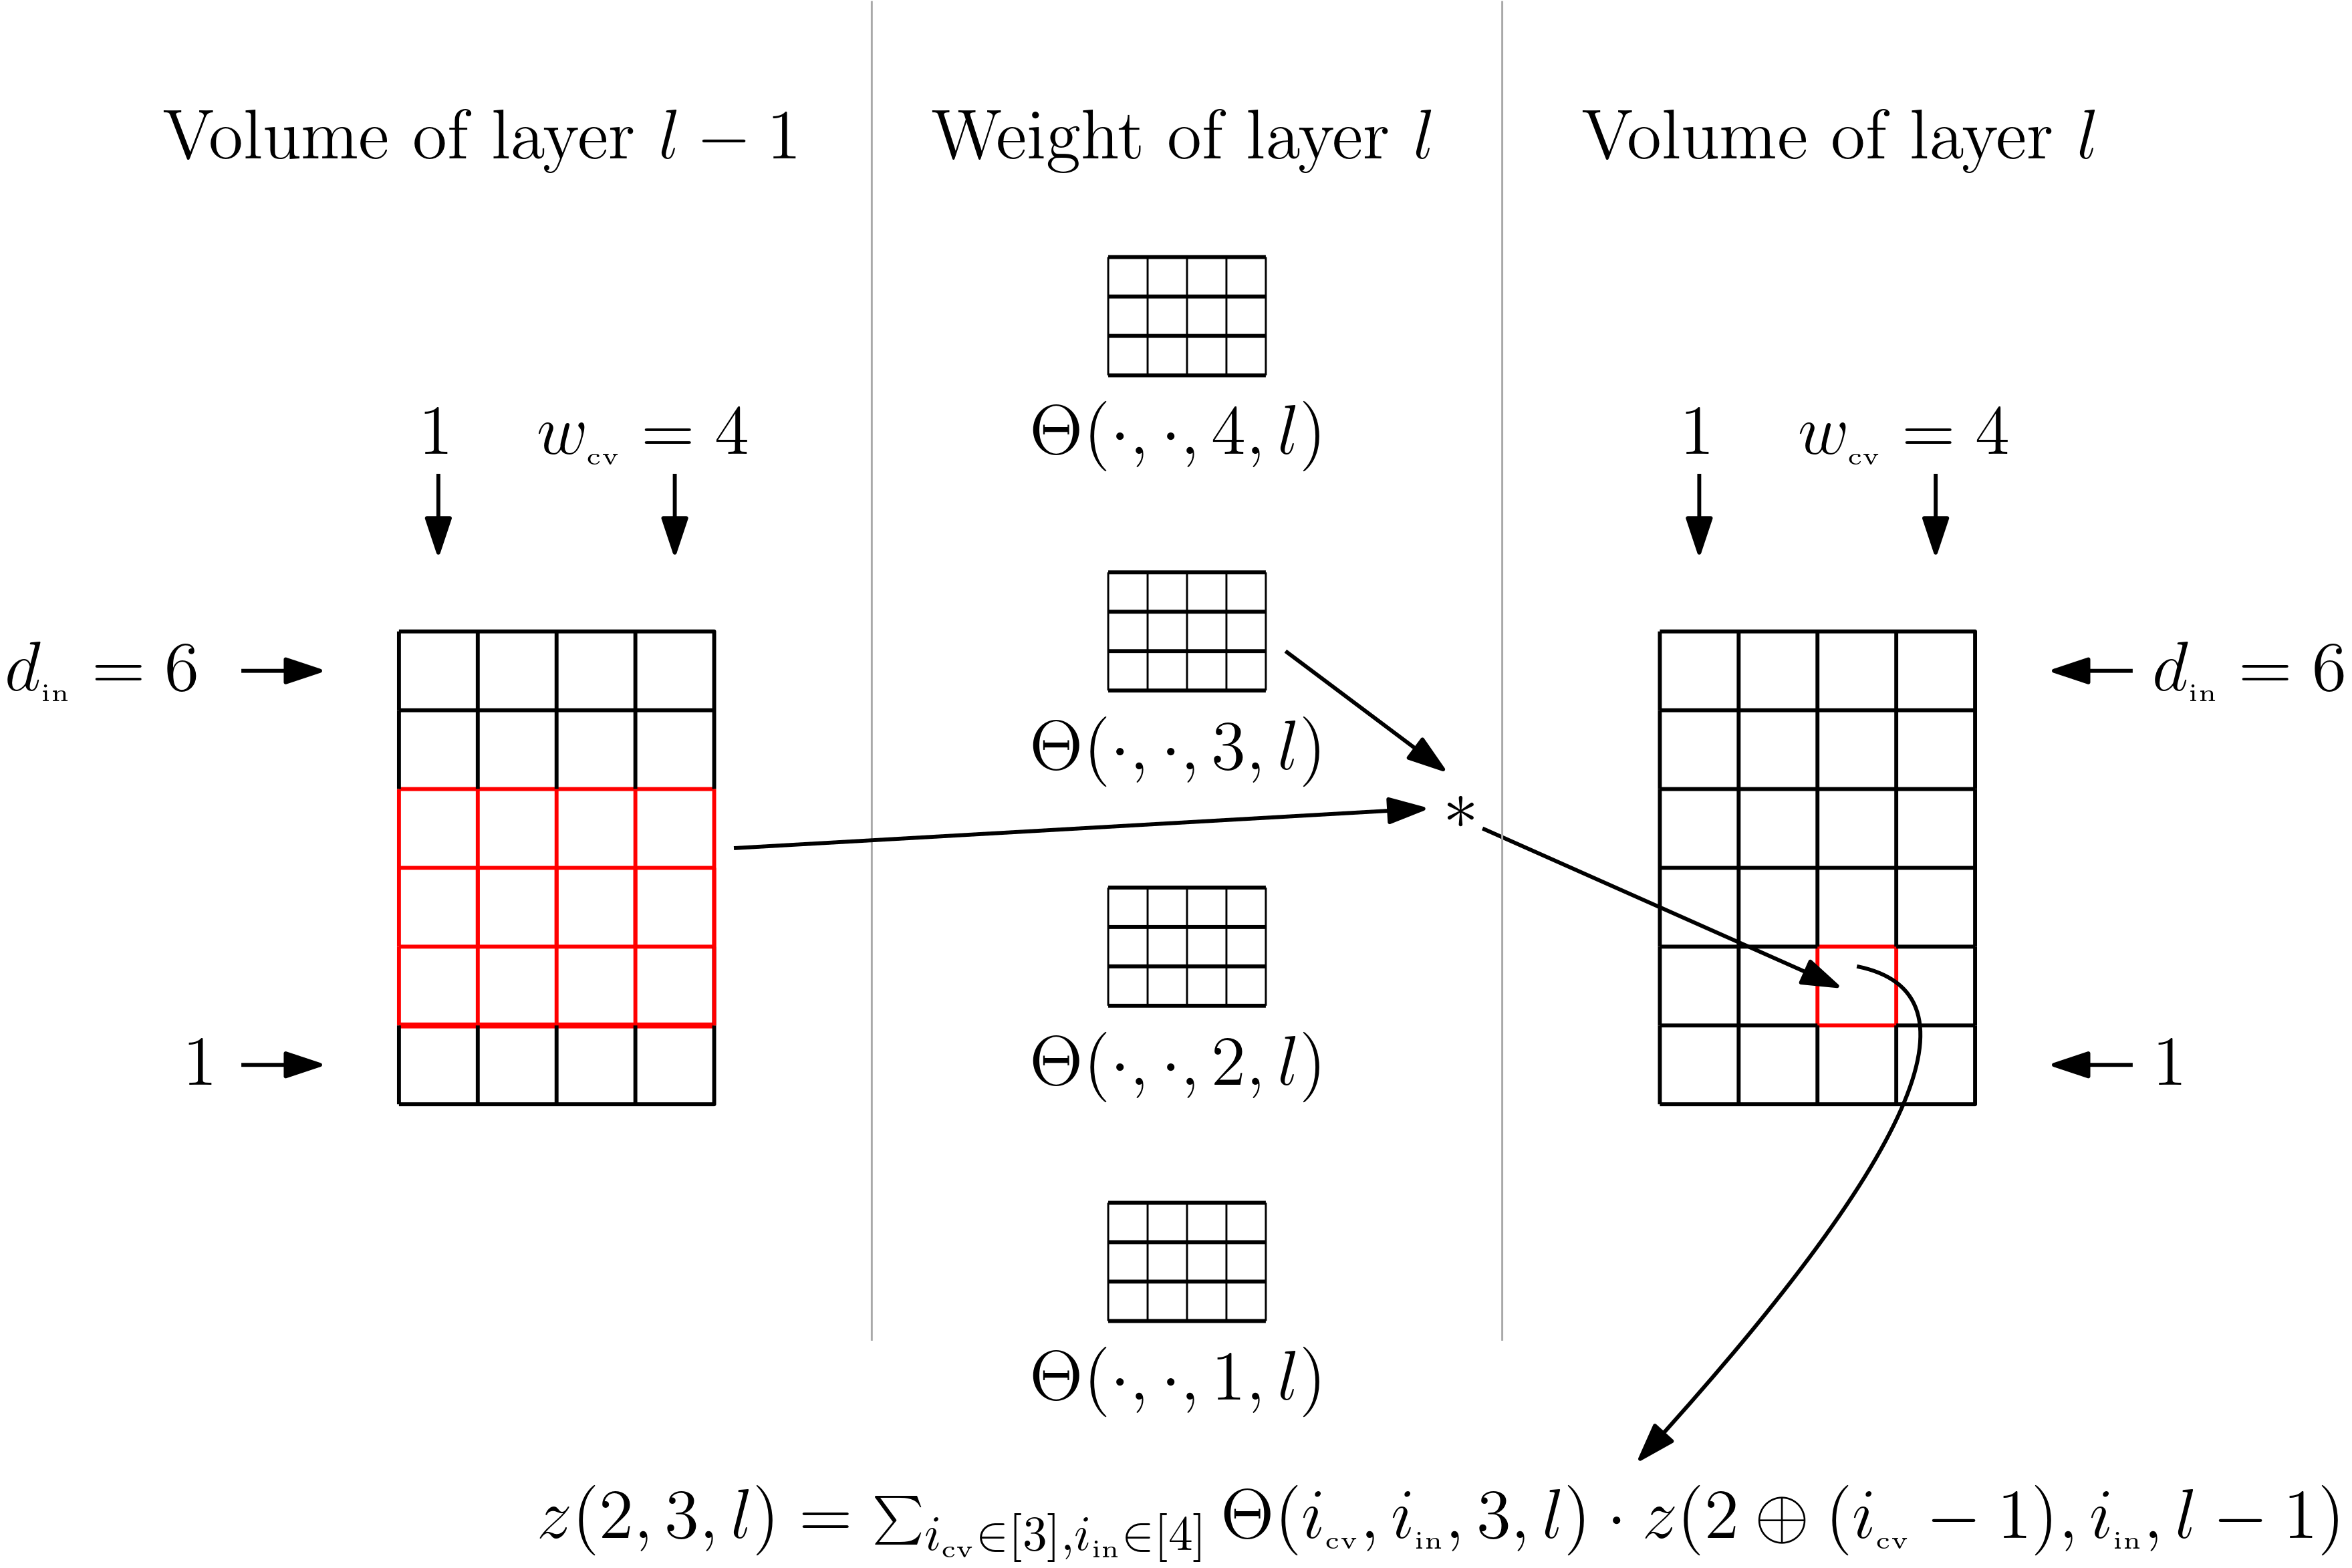
\includegraphics[scale=1]{figs/single-filter.png}
}
\end{figure}
\newpage

%%\input{supp}
%\newpage
\begin{center}
{\Large{\textbf{Appendix}}}
\end{center}

\begin{appendix}
\section{Expression for $K^{(d)}$}\label{sec:kd}
The $K^{(d)}$ matrix is computed by the recursion in \eqref{eq:ntkold}.
\begin{align}\label{eq:ntkold}
&\tilde{K}^{(1)}(s,s')=\Sigma^{(1)}(s,s')=\Sigma(s,s'), M^{(l)}_{ss'}=\left[\begin{matrix}\Sigma^{(l)}(s,s) & \Sigma^{(l)}(s,s')\\ \Sigma^{(l)}(s',s) & \Sigma^{(l)}(s',s')\end{matrix}\right]\in \R^2,\nn\\
&\Sigma^{(l+1)}(s,s')= 2\cdot\mathbb{E}_{(q,q')\sim N(0,M_{ss'}^{(l)})} \left[\chi(q)\chi(q')\right], \hat{\Sigma}^{(l+1)}(s,s')= 2\cdot\mathbb{E}_{(q,q')\sim N(0,M_{ss'}^{(l)})}\left[\partial\chi(q)\partial{\chi}(q')\right],\nn\\
&\tilde{K}^{(l+1)}=\tilde{K}^{(l)}\odot \hat{\Sigma}^{(l+1)}+\Sigma^{(l+1)}, K^{(d)}=\left(\tilde{K}^{(d)}+\Sigma^{(d)}\right)/2
\end{align}
where $s,s'\in[n]$ are two input examples in the dataset, $\Sigma$ is the data Gram matrix, $\partial{\chi}$ stands for the derivative of the activation function with respect to the pre-activation input, $N(0,M)$ stands for the mean-zero Gaussian distribution with co-variance matrix $M$.



\section{Proofs of technical results}
\textbf{Proof of \Cref{prop:basic}}
\begin{proof}
We know that $e_t=(e_t(s),s\in[n])\in\R^n$, and $e_t(s)=\hat{y}_{\Theta_t}(x_s)-y(s)$. Now
\begin{align} 
L_{\Theta_t}&=\frac{1}2\sum_{s'=1}^n(\hat{y}_{\Theta_t}-y)^2\nn\\
&=\frac{1}2\sum_{s'=1}^n e_t^2\nn\\
\nabla_{\Theta} L_{\Theta_t}&= \sum_{s'=1}^n\nabla_{\Theta} \hat{y}_{\Theta_t}(x_{s'})e_t(s')\nn\\
\label{eq:above1} \nabla_{\Theta} L_{\Theta_t}&= \sum_{s'=1}^n \psi_{x_{s'},\Theta_t}e_t(s')
\end{align}
For gradient descent, $\dot{\Theta}_t=-\nabla_{\Theta} L_{\Theta_t}$, from \eqref{eq:above1} it follows that 
\begin{align}
\dot{\Theta}_t=-\sum_{s'=1}^n \psi_{x_{s'},\Theta_t}e_t(s')
\end{align}
Now $\dot{e}_t=\dot{\hat{y}}_{\Theta_t}$, and expanding $\dot{\hat{y}}_{\Theta_t}(x_s)$ for some $s\in[n]$, we have:
\begin{align}
\dot{\hat{y}}_{\Theta_t}(x_s)&=\frac{d \hat{y}_{\Theta_t}(x_s)}{d t}\nn\\
&=\sum_{\theta\in\Theta}\frac{d \hat{y}_{\Theta_t}(x_s)}{d \theta}\frac{d \theta_t}{dt},\,\text{by expressing this summation as a dot product we obtain} \nn\\
\dot{\hat{y}}_{\Theta_t}(x_s)&=\ip{\psi_{x_s,\Theta_t},\dot{\Theta}_t}
\end{align}
We now use that fact that $\Theta_t$ is updated by gradient descent
\begin{align}
\dot{\hat{y}}_{\Theta_t}(x_s)&=-\ip{\psi_{x_s,\Theta_t},\sum_{s'=1}^n \psi_{x_{s'},\Theta_t}e_t(s')}\nn\\
&=-\sum_{s'=1}^n K_{\Theta_t}(s,s')e_t(s')
\end{align}
The proof is complete by recalling that $\hat{y}_{\Theta_t}=(\hat{y}_{\Theta_t}(x_s),s\in[n])$, and $\dot{e}_t=\dot{\hat{y}}_{\Theta_t}$.
\end{proof}


\textbf{Proof of \Cref{prop:zero}}
\begin{proof}
Let $x\in\R^{\din}$ be the input to the DNN and $\hat{y}_{\Theta}(x)$ be its output. The output can be written in terms of the final hidden layer output as:
\begin{align}
\hat{y}_{\Theta}(x)&=\sum_{j_{d-1}=1}^w\Theta(1, j_{d-1},d) \cdot z_{x,\Theta}(j_{d-1},d-1)\nn\\
\label{lastlayer}&=\sum_{j_{d-1}=1}^w\Theta(1, j_{d-1},d) \cdot G_{x\Theta}(j_{d-1},d-1)\cdot q_{x,\Theta}(j_{d-1},d-1)
\end{align}
Now $q_{x,\Theta}(j_{d-1},d-1)$ for a fixed $j_{d-1}$ can again be expanded as
\begin{align}
q_{x,\Theta}(j_{d-1},d-1)&= \sum_{j_{d-2}=1}^w \Theta(j_{d-1},j_{d-2},d-1) \cdot z_{x,\Theta}(j_{d-2},d-2)\nn\\
\label{onebefore}&=\sum_{j_{d-2}=1}^w \Theta(j_{d-1},j_{d-2},d-1) \cdot G_{x,\Theta}(j_{d-2},d-2)\cdot q_{x,\Theta}(j_{d-2},d-2)
\end{align}
Now plugging in \eqref{onebefore} in the expression in \eqref{lastlayer}, we have
\begin{align}
\hat{y}_{\Theta}(x)&=\sum_{j_{d-1}=1}^w\Theta(1, j_{d-1},d)\cdot G_{x\Theta}(j_{d-1},d-1)\Bigg(\sum_{j_{d-2}=1}^w \Theta(j_{d-1},j_{d-2},d-1)\nn\\ &\hspace{15pt}\cdot G_{x,\Theta}(j_{d-2},d-2)\cdot q_{x,\Theta}(j_{d-2},d-2)\Bigg)\nn\\
&=\sum_{j_{d-1}, j_{d-2}\in[w]} G_{x,\Theta}(j_{d-1},d-1)\cdot G_{x,\Theta}(j_{d-2},d-2)\cdot\Theta(1, j_{d-1},d)\nn\\&\cdot \Theta(j_{d-1},j_{d-2},d-1)\cdot q_{x,\Theta}(j_{d-2},d-2)\nn\\
\end{align}
By expanding $q$'s for all the previous layers till the input layer we have
\begin{align}
\hat{y}_{\Theta}(x)=\sum_{j_{d}=1, j_{d-1},\ldots,j_{1}\in[w], j\in[\din]} x(j) \Pi_{l=1}^{d-1}G_{x,\Theta}(j_{l},l) \Pi_{l=1}^{d}\Theta(j_l, j_{l-1}, l) \nn
\end{align}
\end{proof}

\textbf{Proof of \Cref{lm:npk}}
\begin{proof}
\begin{align}
\ip{\phi_{x_s,\Theta},\phi_{x_{s'},\Theta}}&=\sum_{p\in[P]}x_s(\I_0(p))x_{s'}(\I_0(p))A_{\Theta}(x_s,p)A_{\Theta}(x_{s'},p)\nn\\
&=\sum_{i=1}^{\din}x_s(i)x_{s'}(i)\Lambda_{\Theta}(s,s')\nn\\
&=\ip{x_s,x_{s'}}\cdot\Lambda_{\Theta}(s,s')
\end{align}
\end{proof}

    \textbf{Proof of \Cref{prop:ntknew}}
\begin{proof}
Let $\Psi_{\Theta}=(\psi_{x_s,\Theta},s\in[n])\in\R^{\dnet\times n}$ be the NTF matrix, then the NTK matrix is given by $K_{\Theta_t}=\Psi^\top_{\Theta_t}\Psi_{\Theta_t}$. Note that, $\hat{y}_{\Theta}(x_s)=\ip{\phi_{x_s,\Theta},v_{\Theta}}=\ip{v_{\Theta},\phi_{x_s,\Theta}}=v^\top_{\Theta}\phi_{x_s,\Theta}$. Now $\psi_{x_{s},\Theta}=\nabla_{\Theta} v_{\Theta}\phi_{x_s,\Theta}$, and hence $\Psi=\nabla_{\Theta} v_{\Theta}\Phi_{\Theta}$. Hence, $K_{\Theta_t}=\Psi^\top_{\Theta_t}\Psi_{\Theta_t}=\Phi^\top_{\Theta}(\nabla_{\Theta} v_{\Theta})^\top (\nabla_{\Theta} v_{\Theta})\Phi_{\Theta}=\Phi^\top_{\Theta}\V_{\Theta}\Phi_{\Theta}$.
\end{proof}

\textbf{Proof of \Cref{prop:dnnhard}}

\begin{proof}
Follows in a similar manner as the proof of \Cref{prop:basic}.
\end{proof}

\textbf{Proof of {\Cref{prop:condition}}}
\begin{proof}
$\rho_{\min}(K_{\Theta})=\underset{\norm{x}_2=1}{\underset{x\in \R^n}\min}x^\top K_{\Theta} x$. Let $x'\in\R^n$ such that $\norm{x'}_2=1$ and $\rho_{\min}(H_{\Theta})={x'}^\top H_{\Theta} x'$. Now, $\rho_{\min}(K_{\Theta})\leq {x'}^\top K_{\Theta} x'$. 
Let $y'=\Phi x'$, then we have, $\rho_{\min}(K_{\Theta})\leq {y'}^\top \V_{\Theta}y'$. Hence $\rho_{\min}(K_{\Theta})\leq \norm{y'}^2_2 \rho_{\max}(\V_{\Theta})$. Proof is complete by noting that $\norm{y'}^2_2={x'}^\top \Phi^\top_{\Theta}\Phi_{\Theta}x'= \rho_{\min}(H_{\Theta})$.
\end{proof}


\textbf{Proof of \Cref{prop:dgn}}

\begin{proof}
Follows in a similar manner as proof of \Cref{prop:basic}.
\end{proof}

\subsection{Proof of \Cref{th:main}}
\subsubsection{Calculation of $\E{K^\text{v}_{\Tdgn_0}}$}

\begin{proposition}
Let $\tv\in\Tv$ be a weight in layer $l_{\tv}$, and let $p$ be a path that passes through $\tv$. Then 
\begin{align}
\partial_{\tv} v_{\Tv}(p) =& \Pi_{l=1,l\neq l_{\tv}}^{d} \Theta(\I_{l}(p),\I_{l-1}(p),l )
\end{align}
\end{proposition}
\begin{proof}
Proof follows by noting that $v_{\Tv}(p)=\Pi_{l=1}^{d}\Theta(\I_l(p),\I_{l-1}(p),l)$.
\end{proof}


\begin{lemma}\label{lm:dot}
Let $\varphi_{p,\Theta}$ be as in \Cref{def:npvgrad}, under the assumption in ~\Cref{th:main}, for paths $p_1,p_2\in [P], p_1\neq p_2$, at initialisation we have (i) $\E{\ip{\varphi_{p_1,\Tv_0}, \varphi_{p_2,\Tv_0}}}= 0$, (ii) ${\ip{\varphi_{p_1,\Tv_0}, \varphi_{p_1,\Tv_0}}}= d\cdot \sigma^{2(d-1)}$.
\end{lemma}

\begin{proof}
\begin{align*}
\ip{\varphi_{p_1,\Tv_0}, \varphi_{p_2,\Tv_0}}= \sum_{\tv\in \Tv} \partial_{\tv}v_{\Tv_0}(p_1) \partial_{\tv}v_{\Tv_0}(p_2)
\end{align*}
Let $\tv\in\Tv$ be an arbitrary weight. If either $p_1$ or $p_2$ does not pass through $\tv$, then it follows that $\partial_{\tv} v_{\Tv_0}(p_1) \partial_{\tv} v_{\Tv_0}(p_2)=0$. Let us consider the the case when $p_1,p_2$ pass through $\tv$ and without of loss of generality let $\tv$ belong to layer $l_{\tv}\in[d]$. 
  we have
\begin{align*}
&\E{\partial_{\tv}v_{\Tv_0}(p_1)\partial_{\tv}v_{\Tv_0}(p_2)}\\
&=\E{\underset{l\neq l_{\tv}}{\underset{l=1}{\overset{d}{\Pi}}} \Bigg(\Tv_0(\I_{l} (p_1),  \I_{l-1}(p_1),l) \Tv_0(\I_{l}(p_2),\I_{l-1} (p_2),l) \Bigg)}\\
&=\underset{l\neq l_{\tv}}{\underset{l=1}{\overset{d}{\Pi}}}\E{\Tv_0(\I_{l}(p_1),\I_{l-1}(p_1),l)\Tv_0(\I_{l}(p_2),\I_{l-1}(p_2),l)}
\end{align*}
where the $\E{\cdot}$ moved inside the product because at initialisation the weights (of different layers) are independent of each other.
Since $p_1\neq p_2$, there exist a layer $\tilde{l}\in[d],\tilde{l}\neq l_{\tv}$ such that they do not pass through the same weight in layer $\tilde{l}$, i.e., $\Tv_0(\I_{\tilde{l}}(p_1),\I_{\tilde{l}-1}(p_1),\tilde{l},)$ and $\Tv_0(\I_{\tilde{l}}(p_2),\I_{\tilde{l}-1}(p_2),\tilde{l})$ are distinct weights. Using this fact,  we have 
\begin{align*}
&\E{\partial_{\tv}v_{\Tv_0}(p_1)\partial_{\tv}v_{\Tv_0}(p_2)}\\
=&\Bigg(\underset{l\neq l_{\tv},\tilde{l}}{\underset{l=1}{\overset{d}{\Pi}}}\E{\Tv_0(\I_l(p_1), \I_{l-1}(p_1),l)\Tv_0(\I_{l}(p_2),\I_{l-1}(p_2),l)}\Bigg)\\
&\cdot\Bigg(\E{\Tv_0(\I_{\tilde{l}}(p_1),\I_{\tilde{l}-1} (p_1),\tilde{l})}\E{\Tv_0(\I_{\tilde{l}}(p_2), \I_{\tilde{l}-1 }(p_2),\tilde{l})}\Bigg)\\
=&0
\end{align*}

The proof of (ii) is complete by noting that a given path $p_1$ pass through only `$d$' weights, and hence $\sum_{\tv\in\Tv} \partial_{\tv}v_{\Tv_0}(p_1) \partial_{\tv}v_{\Tv_0}(p_1)$ has `$d$' non-zero terms, and the fact that at initialisation we have 
\begin{align*}
&\partial_{\tv}v_{\Tv_0}(p_1) \partial_{\tv}v_{\Tv_0}(p_1) \\
&=\underset{l\neq l_{\tv}}{\underset{l=1}{\overset{d}{\Pi}}} [\Tv_0(\I_{l}(p),\I_{l-1}(p),l)]^2\\
&=\sigma^{2(d-1)}
\end{align*}
\end{proof}



\begin{theorem}\label{th:exp}
 $\E{K^{\text{v}}_{\Tdgn_0}}=d\cdot\sigma^{2(d-1)} \cdot H_{\text{FNPF}}$. 
\end{theorem}
\begin{proof}
Let $\Phi_{\text{FNPF}}=\Phi_{\Tf_0}=\left(\phi_{x_s,\Tf_0}, s\in[n]\right)\in\R^{P\times n}$ be the NPF matrix. 
\begin{align*}
\E{K^{\text{v}}_{\Tdgn_0}}&=\E{\Phi^\top_{\text{FNPF}} \V_{\Tv_0} \Phi_{\text{FNPF}}}\\
&=\E{\Phi^\top_{\text{FNPF}} (\nabla_{\Tv}v_{\Tv_0})^\top (\nabla_{\Tv}v_{\Tv_0}) \Phi_{\text{FNPF}}}\\
&=\Phi^\top_{\text{FNPF}}\left( \E{(\nabla_{\Tv}v_{\Tv_0})^\top (\nabla_{\Tv}v_{\Tv_0})}\right)\Phi_{\text{FNPF}}\\
&\stackrel{(a)}=d\cdot\sigma^{2(d-1)} \cdot\left(\Phi^\top_{\text{FNPF}}\Phi_{\text{FNPF}}\right)\\
&=d\cdot\sigma^{2(d-1)} \cdot H_{\text{FNPF}}
\end{align*}
Here, $(a)$ follows from  \Cref{lm:dot}, i.e., $\E{(\nabla_{\Tv}v_{\Tv_0})^\top (\nabla_{\Tv}v_{\Tv_0})}= d\cdot\sigma^{2(d-1)}\cdot I_{P\times P}$, where $I_{P\times P}$ is a ${P\times P}$ identity matrix.
\end{proof}

\subsubsection{Calculation of $Var\left[K^\text{v}_{\Tdgn_0}\right]$}

\input{varproof}

\textbf{Proof of\Cref{th:main}}
\begin{proof} Follows from \Cref{th:exp} and \Cref{th:var}.
\end{proof}


\section{Applying \Cref{th:main} In Finite Width Case}\label{sec:finite}
In this section, we describe the technical step in applying \Cref{th:main} which requires $w\ra\infty$ to measure the information in the gates of a DNN  with finite width.  Since we are training only the value network in the FPNP mode of the DGN, it is possible to let the width of the value network alone go to $\infty$, while keeping the width of the feature network (which stores the fixed NPFs) finite. This is easily achieved by multiplying the width by a positive integer $m\in\Z_{+}$, and \emph{padding} the gates `$m$' times.
\begin{definition}
Define DGN${}^{(m)}$ to be the DGN whose feature network is of width $w$ and depth $d$, and whose value network  is a fully connected network of width $mw$ and depth $d$. The $mw(d-1)$ gating values are obtained by `padding' the $w(d-1)$gating values of the width `$w$', depth `$d$' feature network `$m$' times (see \Cref{fig:dgnpad}, \Cref{tb:dgnpad}). 
\end{definition}
\FloatBarrier
\begin{table}[h]
\centering
\begin{tabular}{|  l | l |}\hline
 Feature Network (NPF)& Value Network (NPV)\\
 $z^{\text{f}}_{x}(0)=x$ &$z^{\text{v}}_{x}(0)=x$ \\
$q^{\text{f}}_{x}(i,l)=\sum_{j} \Tf(i,j,l)\cdot z_{x}(j,l-1)$ & $q^{\text{v}}_{x}(i,l)=\sum_{j} \Tv(i,j,l)\cdot z^{\text{v}}_{x}(j,l-1)$\\
$z^{\text{f}}_{x}(i,l)= q^{\text{f}}_{x}(i,l)\cdot\mathbbm{1}_{\{q^{\text{f}}_{x}(i,l)>0\}}$& $z^{\text{v}}_{x}(i,l)= q^{\text{v}}_{x}(i,l)\cdot G_{x}(i,l)$ \\
 None &$\hat{y}_{{\Tdgn}^{(m)}}(x)= \sum_{j} \Tv(1,j,l)\cdot z^{\text{v}}_{x}(j,d-1)$\\\hline
\multicolumn{2}{|l|}{{Hard ReLU: $G_{x}(i,l)=\mathbbm{1}_{\{q^{\text{f}}_{x}(i,l)>0\}}$ or Soft-ReLU: $G_{x}(i,l)={1}/{\left(1+\exp(-\beta\cdot q^{\text{f}}_{x}(i,l)>0)\right)} $}}\\\hline
\end{tabular}
\caption{Deep Gated Network with padding. Here the gating values are padded, i.e., $ G_{x}(kw+i,l)=G_{x}(i,l),\forall k=0,1,\ldots,m-1, i\in[w]$. }
\label{tb:dgnpad}
\end{table}



\textbf{Remark:}  DGN${}^{(m)}$ has a total of $P^{(m)}=(mw)^{(d-1)}\din$ paths. Thus, the NPF and NPV are quantities in $\R^{P^{(m)}}$. In what follows, we denote the NPF matrix of DGN${}^{(m)}$ by $\Phi^{(m)}_{\Tf_0}\in\R^{P^{(m)}\times n}$, and use $H^{(m)}_{\text{FNPF}}=(\Phi^{(m)}_{\Tf_0})^\top \Phi^{(m)}_{\Tf_0}$. 

Before we proceed to state the version of \Cref{th:main} for DGN${}^{(m)}$, we will look at an equivalent definition for $\Lambda_{\Theta}$ (see \Cref{def:lambda}).
\begin{definition}\label{def:equilambda}
For input examples $s, s'\in[n]$ define 

$1.$ $\tau_{\Theta}(s,s',l)\stackrel{def}=\sum_{i=1}^w G_{x_s,\Theta}(i,l)G_{x_{s'},\Theta}(i,l)$ be the number of activations that are ``on'' for both inputs $s,s'\in[n]$ in layer $l\in[d-1]$.

$2.$ $\Lambda_{\Theta}(s,s')\stackrel{def}=\Pi_{l=1}^{d-1}\tau_{\Theta}(s,s',l)$.
\end{definition}

\FloatBarrier
\begin{figure}[h]
\centering
%\resizebox{\columnwidth}{\textheight}{
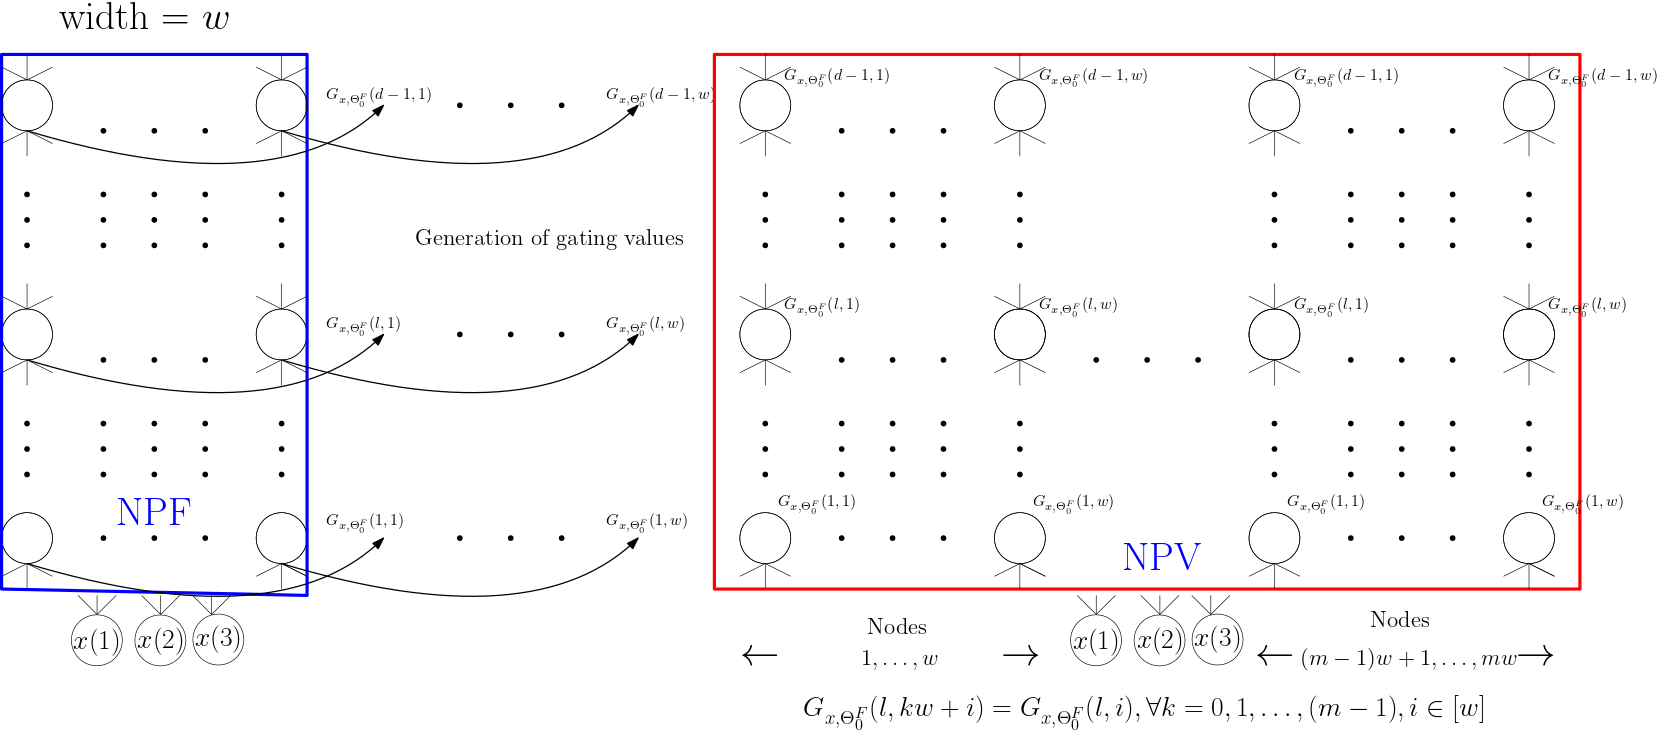
\includegraphics[scale=0.1]{figs/dgn-infty.png}
%}
\caption{DGN${}^{(m)}$ where the value network is of width $mw$ and depth $d$. The gates are derived by padding the gating values obtained from the feature network `$m$' times, i.e., $ G_{x}(kw+i,l)=G_{x}(i,l),\forall k=0,1,\ldots,m-1, i\in[w]$.}
\label{fig:dgnpad}
\end{figure}



\begin{corollary}[Corollary to \Cref{th:main}] Under the same assumptions as in \Cref{th:main} with $\sigma$ replaced by $\sigma_{(m)}=\sigma/\sqrt{m}$, as $m\ra\infty$, \begin{align*}K^{\text{v}}_{\Theta^{\text{DGN}^{(m)}}_0}\ra K^{(d)}_{\text{FNPF}} = d\cdot \sigma_{(m)}^{2(d-1)} H^{(m)}_{\text{FNPF}}= d\cdot \sigma^{2(d-1)} H_{\text{FNPF}}\end{align*}
\end{corollary}
\begin{proof}
Let $\Lambda^{(m)}_{\text{FNPF}}$ and $\tau^{(m)}_{\text{FNPF}}$ be quantities associated with DGN${}^{(m)}$. We know that  $H^{(m)}_{\text{FNFP}}=\Sigma\odot\Lambda^{(m)}_{\text{FNPF}}$. Dropping the subscript FNPF to avoid notational clutter, we have
\begin{align*}
\left(\sigma/\sqrt{m}\right)^{2(d-1)}\Lambda^{(m)}(s,s')&=\sigma^{2(d-1)}\frac{1}{m^{(d-1)}}\Pi_{l=1}^{d-1}\tau^{(m)}(s,s',l)\\
&=\sigma^{2(d-1)}\frac{1}{m^{(d-1)}}\Pi_{l=1}^{d-1}\left(m \tau(s,s',l)\right)\\
&=\sigma^{2(d-1)}\frac{1}{m^{(d-1)}}m^{(d-1)}\Pi_{l=1}^{d-1} \tau(s,s',l)\\
&=\sigma^{2(d-1)}\Pi_{l=1}^{d-1} \tau(s,s',l)\\
&=\sigma^{2(d-1)}\Lambda(s,s')
\end{align*}
\end{proof}


\section{DGN as a Lookup Table: Applying \Cref{th:main} to a pure memorisation task}\label{sec:mem}

In this section, we modify the DGN in \Cref{fig:dgn} into a memorisation network to solve a pure memorisation task. The objective of constructing the memorisation network is to understand the roles of depth and width in \Cref{th:main} in a simplified setting. In this setting, we show increasing depth till a point helps in training and increasing depth beyond it hurts training. 

\begin{definition}[Memorisation Network/Task]
Given a set of values $(y_s)_{s=1}^n\in  \R$, a memorisation network (with weights $\Theta\in\R^{\dnet}$) accepts $s\in[n]$ as its input and produces $\hat{y}_{\Theta}(s)\approx y_s$ as its output. The loss of the memorisation network is defined as $L_{\Theta}=\frac{1}{2}\sum_{s=1}^n (\hat{y}_{\Theta}(s)-y_s)^2$.
\end{definition}
\FloatBarrier
\begin{table}[h]
\centering
\begin{tabular}{| l |  l  |}\hline
Layer&  Memorisation Network\\\hline
Input  &$z_{\Theta}(0)=1$ \\
Pre-Activation & $q_{s,\Theta}(l)=\sum_{j}\Theta(i,j,l)\cdot z_{s,\Theta}(j,l-1)$\\
Hidden & $z_{s,\Theta}(i,l)=q_{s,\Theta}(i,l)\cdot G_{s}(i,l)$ \\
Final  Output & $\hat{y}_{\Theta}(s)=\sum_{j} \Theta(1,j,d) \cdot z_{s,\Theta}(j,d-1)$\\\hline
\end{tabular}
\caption{ Memorisation Network. The input is fixed and is equal to $1$. All the internal variables depend on the index $s$ and the parameter $\Theta$. The gating values $G_s(i,l)$ are external and independent variables.}
\label{tb:dgnmemo}
\end{table}

\textbf{Fixed Random Gating:} The memorisation network is described in \Cref{tb:dgnmemo}. In a memorisation network, the gates are \emph{fixed and random}, i.e., for each index $s\in[n]$, the gating values $G_{s}(i,l),\forall l\in[d-1], i\in[w] $ are sampled from $Ber(\mu), \mu\in(0,1)$ taking values in $\{0,1\}$,  and kept fixed throughout training. The input to the memorisation network is fixed as $1$, and since the gating is fixed and random there is a separate random sub-network to memorise each target $y_s\in\R$. The memorisation network can be used to memorise the targets  $(y_s)_{s=1}^n$ by training it using gradient descent by minimising the squared loss $L_{\Theta}$. In what follows, we let $K_0$ and $H_0$ to be the NTK and NPK of the memorisation network at initialisation.


\textbf{Performance of Memorisation Network:} From \Cref{prop:basic} we know that as $w\ra\infty$, the training error dynamics of the memorisation network follows:
\begin{align}
\dot{e}_t=-K_{0} e_t,
\end{align}
i.e., the spectral properties of $K_0$ (or $H_0$) dictates the rate of convergence of the training error to $0$. In the case of the memorisation network with fixed and random gates, we can calculate $\E{K_0}$ explicitly. 

\textbf{Spectrum of $H_0$:} The input Gram matrix $\Sigma$ is a $n\times n$ matrix with all entries equal to $1$ and its rank is equal to 1, and hence $H_0=\Lambda_0$. We can now calculate the properties of $\Lambda_0$. It is easy to check that $\mathbb{E}_{\mu}\left[\Lambda_0(s,s)\right]=(\mu w)^{(d-1)},\forall s\in[n]$ and $\mathbb{E}_{\mu}\left[\Lambda_0(s,s')\right]=(\mu^2 w)^{(d-1)},\forall s,s'\in[n]$.  For $\sigma=\sqrt{\frac{1}{\mu w}}$, and $\mathbb{E}_{\mu}\left[K_0(s,s)/d\right]=1$, and $\mathbb{E}_{\mu}\left[K_0(s,s')/d\right]=\mu^{(d-1)}$. 
\begin{figure}
\centering
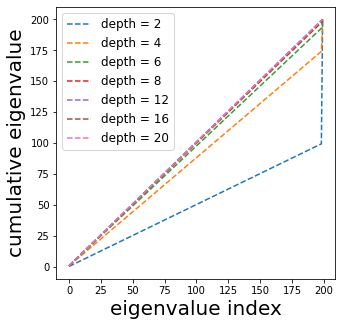
\includegraphics[scale=0.3]{figs/dgn-fra-ecdf-ideal-small.png}
\caption{Ideal spectrum of $\E{K_0}/d$ for a memorisation network for $n=200$.}
\label{fig:ideal-spectrum}
\end{figure}


\textbf{Why increasing depth till a point helps ?} 
We have:
%\comment{
\begin{align}\label{eq:mat}
\frac{\E{K_0}}{d}=\left[\begin{matrix}
1 &\mu^{d-1} &\ldots &\mu^{d-1} &\ldots\\ 
\ldots &1 &\ldots &\mu^{d-1} &\ldots\\ 
\ldots &\mu^{d-1} &\ldots &1 &\ldots \\
\ldots &\mu^{d-1} &\ldots &\mu^{d-1} &1\\ 
\end{matrix}\right]
\end{align}
%}
i.e., all the diagonal entries are $1$ and non-diagonal entries are $\mu^{d-1}$. Now, let $\rho_i\geq 0,i \in [n]$ be the eigenvalues of $\frac{\E{K_0}}{d}$, and let $\rho_{\max}$ and $\rho_{\min}$ be the largest and smallest eigenvalues.  One can easily show that $\rho_{\max}=1+(n-1)\mu^{d-1}$ and corresponds to the eigenvector with all entries as $1$, and $\rho_{\min}=(1-\mu^{d-1})$ repeats $(n-1)$ times,  which corresponds to eigenvectors given by $[0, 0, \ldots, \underbrace{1, -1}_{\text{$i$ and $i+1$}}, 0,0,\ldots, 0]^\top \in \R^n$ for $i=1,\ldots,n-1$. Note that as $d\ra\infty$, $\rho_{\max},\rho_{\min}\ra 1$.

\textbf{Why increasing depth beyond a point hurts?} 
As the depth increases the variance of the entries $K_0(s,s')$ deviates from its expected value $\E{K_0(s,s')}$. Thus the structure of the Gram matrix degrades from \eqref{eq:mat}, leading to smaller eigenvalues.
%\FloatBarrier
\begin{figure}
\resizebox{\textwidth}{!}{
\begin{tabular}{cccc}
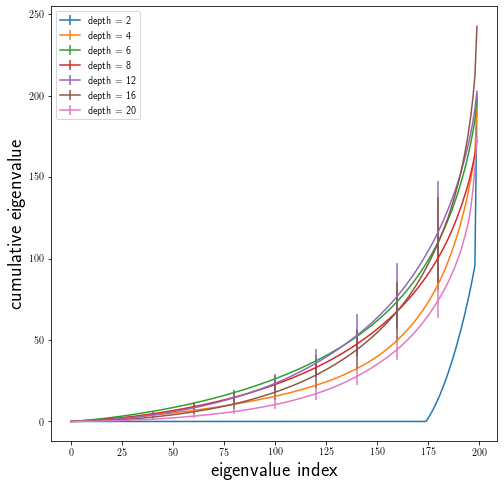
\includegraphics[scale=0.5]{figs/dgn-fra-ecdfbyd-w25.png}
&
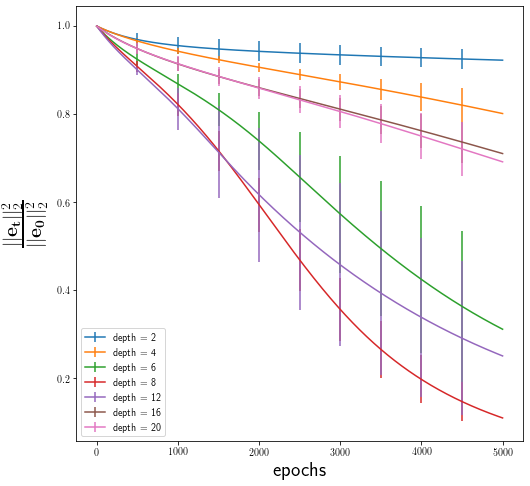
\includegraphics[scale=0.5]{figs/dgn-fra-conv-w25.png}
&
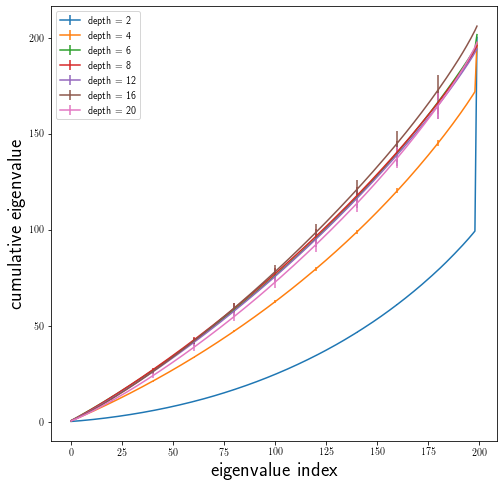
\includegraphics[scale=0.5]{figs/dgn-fra-ecdfbyd-w500.png}
&
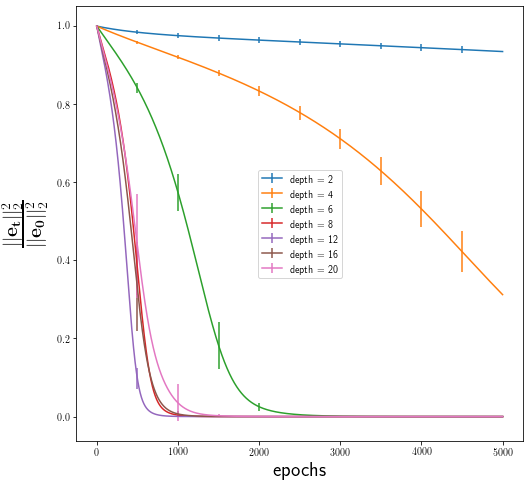
\includegraphics[scale=0.5]{figs/dgn-fra-conv-w500.png}
\end{tabular}
}
\caption{Shows the plots for the memorisation network with $\mu=\frac{1}{2}$ and $\sigma=\sqrt{\frac{2}{w}}$. The number of points to be memorised is $n=200$. The left most plot shows the e.c.d.f for $w=25$ and the second plot from the left shows the error dynamics during training for $w=25$. The second plot from the right shows the e.c.d.f for $w=500$ and the right most plot shows the error dynamics during training for $w=500$. All plots are averaged over $10$ runs.}
\label{fig:dgn-frg-gram-ecdf}
\end{figure}

\subsection{Experiment}
We set $n=200$, and $y_s\sim\text{Uniform}[-1,1]$. We look at the cumulative eigenvalue (e.c.d.f) obtained by first sorting the eigenvalues in ascending order then looking at their cumulative sum. The ideal behaviour (\Cref{fig:ideal-spectrum}) as predicted from theory is that for indices $k\in[n-1]$, the e.c.d.f should increase at a linear rate, i.e., the cumulative sum of the first $k$ indices is equal to $k(1-\mu^{d-1})$, and the difference between the last two indices is $1+(n-1)\mu^{d-1}$. In \Cref{fig:dgn-frg-gram-ecdf}, we plot the actual e.c.d.f for various depths $d=2,4,6,8,12,16,20$ and $w=25,500$ (first and third plots from the left in \Cref{fig:dgn-frg-gram-ecdf}). 

\textbf{Roles of depth and width:} In order to compare how the rate of convergence varies with the depth, we set the step-size $\alpha=\frac{0.1}{\rho_{\max}}$, $w=100$. We use the vanilla SGD-optimiser. Note the$ \frac{1}{\rho_{\max}}$ in the stepsize, ensures that the uniformity of maximum eigenvalue across all the instances, and the convergence should be limited by the smaller eigenvalues. We also look at the convergence rate of the ratio $\frac{\norm{e_t}^2_2}{\norm{e_0}^2_2}$. We notice that for $w=25$, increasing depth till $d=8$ improves the convergence, however increasing beyond $d=8$ worsens the convergence rate. For $w=500$, increasing the depth till $d=12$ improves convergence, and $d=16,20$ are worse than $d=12$.  %This matches with the depth phenomena observed in practical DNNs and also matches our theory.
\end{appendix}

\end{document}
